%%%%%%%%%%%%%%%
%
% $Autor: Wings $
% $Datum: 2020-01-29 07:55:27Z $
% $Pfad: komponenten/Bilderkennung/Produktspezifikation/IntelNCS2/IntelNCS2.tex $
% $Version: 1785 $
%
%
%%%%%%%%%%%%%%%


% Auswahl der Sprache
% Die nicht gewünschte Sprache muss auskommentiert werden:
%\def\isGerman{1}
\def\isEnglish{1}


\documentclass[10pt,a4paper,bibliography=totoc]{scrbook}

%%%%%%%%%%%%%%%%%%%%%%%%%%%%%%
%
% $Autor: Wings $
% $Datum: 2020-01-30 07:43:10Z $
% $Pfad: komponenten/Bilderkennung/Produktspezifikation/JetsonNano/Allgemein/packages.tex $
% $Version: 1786 $
%
%
%%%%%%%%%%%%%%%%%%%%%%%%%%%%%%




\usepackage[left=4cm,right=4cm,top=2cm,bottom=2cm,includeheadfoot]{geometry}
\setlength{\headheight}{1pt}

% Standard Deutsch
\usepackage{lmodern}
\usepackage[utf8]{inputenc}
\ifdefined\isGerman
  \usepackage[ngerman]{babel}
\else
  \ifdefined\isEnglish
    \usepackage[english]{babel}
  \else
    \usepackage[ngerman]{babel}
  \fi
\fi

\usepackage[T1]{fontenc}

% Farben
\usepackage{xcolor}
\usepackage{alltt}
% Notwendig für Syntax-Highlighting mit besonderen Farben
%\usepackage[table, x11names]{xcolor}
\usepackage{color}
\usepackage{soul}

% Pakete für Mathe
\usepackage{amsmath}
\usepackage{amsfonts}
\usepackage{amssymb}
\usepackage{mathtools}


% Paket Internetrefferenzen
\usepackage{hyperref}

%Wird zusätzlich das Paket showidx eingebunden, werden die gesetzten Einträge am Seitenrand dargestellt. 
\usepackage{imakeidx}
%\usepackage{showidx}
%\usepackage[override=false]{seealso}
\makeindex[intoc,title=Index]
\ifdefined\isGerman
  \renewcommand{\indexname}{Stichwortverzeichnis}
\else
\ifdefined\isEnglish
\else
  \renewcommand{\indexname}{Stichwortverzeichnis}
\fi
\fi




% Paktete für Bilder
\usepackage{graphicx}

\usepackage{listings}
% Automatische erstellung von Referenzen
\usepackage[ngerman]{cleveref}
% Zeilenumbrüche in \texttt
\usepackage[htt]{hyphenat}

% Automatisches erstellen und referenzieren eines Abkürzungsverzeichnisses
\usepackage[tooltip]{acro}
% Ermöglicht Verwendung von 'H' Float modifier
\usepackage{float}

% Ermöglicht Subfigures und Subcaptions
\usepackage{subcaption}


\usepackage{float}
\usepackage{array}
\usepackage{amsopn}
\usepackage[percent]{overpic}
\usepackage{colortbl}
\usepackage{marginnote}

\usepackage{textcomp}

\usepackage[
backend=bibtex8,%  defernumbers=true,
autocite=inline,
labelalpha=true,%  sorting=none,
firstinits=true,
uniquename=init,
uniquelist=false,
refsegment=section,
style=alphabetic,
safeinputenc
]{biblatex}

%\usepackage[german]{babelbib}
%\usepackage[square,sort,comma,numbers]{natbib}
%\DeclareNameAlias{sortname}{last-first}
%\bibliographystyle{geralpha}
%\setcitestyle{square,aysep={},yysep={;}}
%\newcommand*{\multicitedelim}{\addsemicolon\space}


% Verwendung:
%\Ausblenden{.....
%} %todo Ausblenden



% Kapitel entfernen
%\usepackage{titlesec}

\usepackage{tabularx} 
\usepackage{longtable}
\usepackage{framed}
\usepackage{tocbibind}

\usepackage[official]{eurosym}

\definecolor{mygreen}{rgb}{0,0.6,0}
\definecolor{mygray}{rgb}{0.5,0.5,0.5}
\definecolor{mymauve}{rgb}{0.58,0,0.82}


%\usepackage{pythonhighlight}


\pagestyle{empty}




% Kopfzeile
\usepackage{fancyhdr}
\pagestyle{fancy}
\fancyhf{}
\fancyhead[OL]{\nouppercase{\leftmark}}
\fancyhead[OR]{\thepage}
\fancyhead[ER]{\nouppercase{\leftmark}}
\fancyhead[ER]{\nouppercase{\chaptermark{}}}
\fancyhead[ER]{\nouppercase{\chaptermark{}}}
\fancyhead[EL]{\thepage}
\renewcommand{\headrulewidth}{0.1pt} 



%\AtBeginDocument{\renewcommand{\chaptername}{}} % muss nach babel stehen! 



\usepackage{ifthen}

\usepackage{media9}
\usepackage{animate}
\newcounter{AnimateAngle}
\setcounter{AnimateAngle}{0}
\newcounter{AnimateStepFactor}
\setcounter{AnimateStepFactor}{1}
\newcounter{AnimateSteps}
\setcounter{AnimateSteps}{0}


\usepackage{multirow}                  % Tabelle vertikale Zellen verbinden
\usepackage{rotating}                  % text rotieren \rotatebox{90}{text}
\usepackage{colortbl}                  % Farbe der Zellen einer Tabelle, z. B. \begin{tabular}{c>{\columncolor{green}}cc}

\usepackage{enumitem}
\usepackage{spverbatim}

% Korrekte darstellung von SI-Einheiten
\usepackage[binary-units=true, per-mode=symbol]{siunitx}
% Erstellen einer ToDo-Liste
\usepackage[ngerman, colorinlistoftodos]{todonotes}
% Kommando zum markieren fehlender praktischer Umsetzungen
\newcommand{\todop}[2][]{\todo[color=red, inline, #1]{#2}}
\usepackage{makecell}
% Bera Mono als \ttfamily font
\usepackage[scaled]{beramono}

\usepackage{menukeys}
\usepackage{textcomp}


% Add section names to todonotes list
\makeatletter
\let\ori@chapter\@chapter
\def\@chapter[#1]#2{\ori@chapter[#1]{#2}%
    \if@mainmatter\addcontentsline{tdo}{chapter}{\protect\numberline{\thechapter}{#1}}%
    \else\addcontentsline{tdo}{chapter}{#1}%
    \fi}
\makeatother

% Farben für Syntax-Highlighting
\definecolor{dkgreen}{rgb}{0,.6,0}
\definecolor{dkblue}{rgb}{0.655,0.113,.364}
\definecolor{dkyellow}{cmyk}{0,0,.8,.3}

\definecolor{parameterc}{rgb}{.4,0,.6}
\definecolor{typec}{rgb}{0,0.525,.702}
\definecolor{stringc}{rgb}{0,.5019,.5019}
\definecolor{keywordc}{rgb}{.6549, .1137, .3647}
\definecolor{commentc}{rgb}{.5882, .5960, .5882}
\definecolor{textc}{rgb}{.2,.2,.2}

\lstdefinestyle{all}{
    alsoletter={-},
    frame=single, 	% top,frame=bottom,
    numbers=none,
    numberstyle=\tiny\color{textc},
    basicstyle=\linespread{0.9}\ttfamily\footnotesize\color{textc},
    tabsize=4,
    showstringspaces=false,
    captionpos=t,
    rulecolor=\color{lightgray!40},
    keywordstyle=\color{keywordc},
    stringstyle=\color{stringc},
    commentstyle=\color{commentc},
    breaklines=true,
    escapechar="!",
    postbreak=\mbox{\textcolor{green}{$\hookrightarrow$}\space},
}

\lstdefinestyle{bashstyle}{
    style=all,
    keywords=[2]{-y, --no-install-recommends, --allow-change-held-packages, --allow-downgrades, --fetch-keys, -n, --version, --params, -c, -i, -O, --upgrade, --no-cache-dir, --extra-index-url, --show, -s, -m},
    keywordstyle=[2]\color{parameterc},
    morekeywords = {ln,choco,pip,pip3,apt,apt-key,apt-get,apt-mark,add-apt-repository,wget,mktemp,dpkg,dpkg-query,echo,>>,rm,tegrastats, systemctl},
    deletekeywords={local,LOCAL},
}

\lstdefinestyle{pythonstyle}{
    style=all,
    morekeywords={as},
    keywords=[2]{True, False, None},
    keywordstyle=[2]\color{typec},
    alsoletter={_},
    keywords=[3]{max_workspace_size_bytes, precision_mode, maximum_cached_engines, use_calibration, optimizer, loss, input_shape, from_logits, metrics, batch_size, epochs, validation_data, activation, use_calibration, filters, kernel_size, pool_size, units},
    keywordstyle=[3]\color{parameterc},
    deletekeywords={compile,COMPILE},
}

\lstdefinestyle{inlinestyle}{
    style=all,
    breaklines        = true,
    breakatwhitespace = true,
    breakindent       = 2ex,
    escapechar        = *,
    numbers           = left,
    postbreak=,
}
\lstdefinelanguage{MyBash} {
    language = Bash,
    style=bashstyle,
}

\lstdefinelanguage{MyPython} {
    language = Python,
    style=pythonstyle,
}

\usepackage[intoc]{nomencl}
\renewcommand{\nomname}{Symbolverzeichnis}
\renewcommand{\nomlabel}[1]{#1 \dotfill}
\makenomenclature

\usepackage{enumitem,amssymb}
\newlist{todolist}{itemize}{2}
\setlist[todolist]{label=$\square$}

\usepackage{blindtext}
%%%%%%
%
% $Autor: Wings $
% $Datum: 2020-01-18 11:15:45Z $
% $Pfad: WuSt/Skript/Produktspezifikation/powerpoint/ImageProcessing.tex $
% $Version: 4620 $
%
%%%%%%



\graphicspath{%
	{../Images/},{Images/},{../../Images/},%
	{../../../../General/},{../../../General/},{../../General/},%
	{../../../../Aufgaben/},{../../../Aufgaben/},%
	{../}}


\definecolor{MapleColor}{rgb}{1,0.0,0.}
\definecolor{PythonColor}{rgb}{0,0.5,1.}
\definecolor{ShellColor}{rgb}{1,0,0.5}
\definecolor{FileColor}{rgb}{0.5,0.5,1.}


\newcommand{\MapleCommand}[1]{\textcolor{MapleColor}{\texttt{\justify#1}}}
\newcommand{\PYTHON}[1]{\textcolor{PythonColor}{\texttt{\justify#1}}}
\newcommand{\SHELL}[1]{\textcolor{ShellColor}{\texttt{\justify#1}}}
\newcommand{\FILE}[1]{\textcolor{FileColor}{\texttt{\justify#1}}\index{\TRANS{Datei}{File}!#1}}
\newcommand{\PATH}[1]{\textcolor{FileColor}{\texttt{\justify#1}}}

\newcommand{\URL}[1]{\textcolor{blue}{\url{#1}}}
\newcommand{\HREF}[2]{\textcolor{blue}{\href{#1}{#2}}}


\newcommand{\QUELLE}{\textcolor{red}{hier Quelle finden}}

\newcolumntype{L}[1]{>{\raggedright\arraybackslash}p{#1}} % linksbündig mit Breitenangabe

\newcommand{\GRAFIK}{\textcolor{red}{Grafik einfügen}}

\newcommand{\DEF}[1]{\fcolorbox{blue}{blue!10}{\begin{minipage}{\textwidth}\textbf{Definition.}#1\end{minipage}}}

\newcommand{\BEISPIEL}[1]{\fcolorbox{blue}{blue!10}{\begin{minipage}{\textwidth}\textbf{Beispiel.}#1\end{minipage}}}

\newcommand{\SATZ}[1]{\fcolorbox{blue}{blue!10}{\begin{minipage}{\textwidth}\textbf{Satz.}#1\end{minipage}}}

\newcommand{\Bemerkung}[1]{\fcolorbox{blue}{blue!10}{\begin{minipage}{\textwidth}\textbf{Bemerkung.}#1\end{minipage}}}


%Zahlenmengen
\newcommand{\C}{\mathbb{C}}
\newcommand{\R}{\mathbb{R}}
\newcommand{\N}{\mathbb{N}}
\newcommand{\Z}{\mathbb{Z}}
\newcommand{\Q}{\mathbb{Q}}
\newcommand{\Po}{\mathbb{P}}
\newcommand{\Rp}[2]{\mathbb{R}^{[#1;\,#2]}} % Menge der auf [a,b]-periodischen Funktionrn
%\DeclareMathOperator{\arg}{arg}
\newcommand{\MyComplex}[1]{\mathbf{#1}}
\newcommand{\Laplaceinv}[1]{#1}
\newcommand{\Bez}{Bézier}
\newcommand{\PH}{pythagoreische Hodographen \xspace}
\newcommand{\PHd}{pythagoreischen Hodographen \xspace}


\DeclareMathOperator{\Atan2}{Atan2}
\DeclareMathOperator{\sign}{sign}
\DeclareMathOperator{\ReLU}{ReLU}

\newcommand*\justify{%
	\fontdimen2\font=0.4em% interword space
	\fontdimen3\font=0.2em% interword stretch
	\fontdimen4\font=0.1em% interword shrink
	\fontdimen7\font=0.1em% extra space
	\hyphenchar\font=`\-% allowing hyphenation
}

% Auswahl der Sprache
% 1.Argument ist der Pfad ohne "en" oder "de"
% 2.Argument ist der Dateiname
\newcommand{\InputLanguage}[2]{
    \ifdefined\isGerman
    \input{#1de/#2}
    \else
    \ifdefined\isEnglish
    \input{#1en/#2}
    \else
    \input{#1de/#2}
    \fi
    \fi
}

\newcommand{\TRANS}[2]{
    \ifdefined\isGerman
    #1%
    \else
    \ifdefined\isEnglish
    #2%
    \else
    #1%
    \fi
    \fi
}


% muss für Akronyme \ac statt see verwendet werden.
\newcommand{\Siehe}{
    \ifdefined\isGerman
    \emph{siehe}
    \else
    \ifdefined\isEnglish
    \emph{see}
    \else
    \emph{siehe}
    \fi
    \fi
}

\renewcommand{\indexname}{
	\ifdefined\isGerman
	\emph{Stichwortverzeichnis}
	\else
	\ifdefined\isEnglish
	\emph{Index}
	\else
	\emph{Stichwortverzeichnis}
	\fi
	\fi
}


%todo Die Kommandos sind für das Endprodukt zu entfernen. Die entsprechenden Stellen sind zu bearbeiten bzw. zu löschen
\newcommand{\Mynote}[1]{\marginnote{\textcolor{red}{WS:#1}}}
\newcommand{\Ausblenden}[1]{}
\newcommand{\ToDo}[1]{\textcolor{red}{\section{ToDo} #1}}

\newcommand{\GRAFIKEINFUEGEN}{\textcolor{red}%
	{\bf Hier ist eine Grafik einzufügen}}
\newcommand{\neu}{\textcolor{red}{Wort Einfügen}}
\newcommand{\REFERENZ}{\textcolor{red}%
	{\bf Referenz  einzufügen}}
\newcommand{\EXAMPLE}{\textcolor{red}%
	{\bf Beispiel einzufügen}}

\newcommand{\trinom}[3]{\left(\begin{array}{c} #1\\#2\\#3 \\ \end{array}\right)}


\newcommand{\textdirectcurrent}{%
	\settowidth{\dimen0}{$=$}%
	\vbox to .85ex {\offinterlineskip
		\hbox to \dimen0{\leaders\hrule\hfill}
		\vskip.35ex
		\hbox to \dimen0{%
			\leaders\hrule\hskip.2\dimen0\hfill
			\leaders\hrule\hskip.2\dimen0\hfill
			\leaders\hrule\hskip.2\dimen0
		}
		\vfill
	}%
}
\newcommand{\mathdirectcurrent}{\mathrel{\textdirectcurrent}}

\newlist{notes}{enumerate}{1}
\setlist[notes]{label=Note: ,leftmargin=*}

% Kommandos für In-Line Code
\newcommand{\COMMAND}[1]{\lstinline[language=MyBash, style=inlinestyle]{#1}}
\newcommand{\mytt}[1]{\texttt{\footnotesize #1}}
\newcommand{\python}[1]{\lstinline[language=MyPython, style=inlinestyle]{#1}}
\newcommand{\twod}[2]{
	\ensuremath{{#1} \times {#2}}}
\newcommand{\threed}[3]{
	\ensuremath{{#1} \times {#2} \times {#3}}}

% Fett-geschriebene Tabellenberschriften
\renewcommand\theadfont{\bfseries}


\newcommand{\us}{\si{\micro\second}}
\newcommand{\usn}[1]{\SI{#1}{\micro\second}}
\renewcommand{\textapprox}{\raisebox{0.5ex}{\texttildelow}}



% Fehlerzähler
\setul{0.5ex}{0.3ex}
\setulcolor{red}
\newcounter{fehlernummer}
\setcounter{fehlernummer}{11}
\newcommand{\FEHLER}[1]{\ul{#1}\stepcounter{fehlernummer}\textsuperscript{\textcolor{red}{\arabic{fehlernummer}}}}
%\renewcommand{\FEHLER}[1]{\ul{#1}\stepcounter{fehlernummer}\marginnote{\textcolor{red}{\arabic{fehlernummer}}}} geht leider nicht
%\renewcommand{\FEHLER}[1]{\ul{#1}\stepcounter{fehlernummer}\footnote{\textcolor{red}{\arabic{fehlernummer}.Fehler}}} geht leider nicht


\newcounter{FortlaufendeNummer}
\setcounter{FortlaufendeNummer}{1}
\newcounter{LetztesKapitel}
\setcounter{LetztesKapitel}{-1}

\newcounter{BeamerChapter}
\setcounter{BeamerChapter}{1}


\newcommand{\GRAPHICSC}[3]{\begin{center}
		\includegraphics[scale=#1]{#3}
\end{center}}

\newcommand{\GRAPHICS}[3]{\includegraphics[scale=#1]{#3}}

\newcommand{\FONO}{   
	%\ifthenelse{\value{chapter} > \value{LetztesKapitel}}%
	%{%
		%\setcounter{LetztesKapitel}{\value{chapter}}%
		%\setcounter{FortlaufendeNummer}{1}%
		%}%
	%\arabic{chapter}.\arabic{FortlaufendeNummer}.%
	%\stepcounter{FortlaufendeNummer}%
}

\newcommand{\FONOBEAMER}{%
	\ifthenelse{\value{BeamerChapter}>0}%
	{%
		\ifthenelse{\value{BeamerChapter}>\value{LetztesKapitel}}%
		{%
			\setcounter{LetztesKapitel}{\value{BeamerChapter}}%
			\setcounter{FortlaufendeNummer}{1}%
		}%
		\hbox{}\arabic{BeamerChapter}.\arabic{FortlaufendeNummer}.\stepcounter{FortlaufendeNummer}%
	}%
	\hbox{}%
} 


\newcommand{\FONOBEAMERSTEP}{%
	\ifthenelse{\value{BeamerChapter}>0}%
	{%
		\ifthenelse{\value{BeamerChapter}>\value{LetztesKapitel}}%
		{%
			\setcounter{LetztesKapitel}{\value{BeamerChapter}}%
			\setcounter{FortlaufendeNummer}{1}%
		}%
		\stepcounter{FortlaufendeNummer}%
	}%
	\hbox{}%
	\bigskip
} 

\newcommand{\FONOBEAMERSTAY}{   
	\ifthenelse{\value{BeamerChapter}>\value{LetztesKapitel}}
	{
		\setcounter{LetztesKapitel}{\value{BeamerChapter}}
		\setcounter{FortlaufendeNummer}{1}
	}
	\hbox{}\arabic{BeamerChapter}.\arabic{FortlaufendeNummer}.} 


% \FONOBEAMERSTEP
% \SATZNAME{}{}
% \SATZ{}
% \SATZNAMES{}{}
% \SATZS{}
% \STANDARD{}{}
% \STANDARDN{}{}  handout:0
% \STANDARDV{}{}  verbatim
% \DEF{}
% \DEFNAME{}{}
% \DEFS{}
% \DEFNAMES{}{}
% \BEMERKUNG{}
% \BEMERKUNGNAME{}{}
% \BEMERKUNGNAMES{}{}
% \BEISPIELNAME{}{}
% \BEISPIELNAMES{}{}
% \BEISPIEL{}
% \BEISPIELS{}



\newcommand{\Def}[1]
{
	\definecolor{shadecolor}{rgb}{0.98, 0.91, 0.71}
	
	\begin{snugshade*}
		\textbf{\FONOBEAMER  Definition.} #1
	\end{snugshade*}
	
	\bigskip
}

\newcommand{\DefN}[2]
{
	\definecolor{shadecolor}{rgb}{0.98, 0.91, 0.71}
	
	\begin{snugshade*}
		\textbf{ \FONOBEAMER Definition #1.}  #2
	\end{snugshade*}
	
	\bigskip
}


\newcommand{\Satz}[1]
{
	\definecolor{shadecolor}{rgb}{0.74, 0.83, 0.9}
	
	\begin{snugshade*}
		\textbf{\FONOBEAMER  Satz.} #1
	\end{snugshade*}
	
	\bigskip
}

\newcommand{\SatzN}[2]
{
	\definecolor{shadecolor}{rgb}{0.74, 0.83, 0.9}
	
	\begin{snugshade*}
		\textbf{ \FONOBEAMER Satz #1.}  #2
	\end{snugshade*}
	
	\bigskip
}


\newcommand{\BemerkungN}[2]
{
	\definecolor{shadecolor}{rgb}{0.66, 0.89, 0.63} %Lavendel
	
	\begin{snugshade*}
		\textbf{ \FONOBEAMER Bemerkung #1.}  #2
	\end{snugshade*}
	
	\bigskip
}


\newcommand{\Beispiel}[1]
{
	\definecolor{shadecolor}{rgb}{0.9, 0.9, 0.98} 
	
	\begin{snugshade*}
		\textbf{\FONOBEAMER  Beispiel.} #1
	\end{snugshade*}
	
	\bigskip
}

\newcommand{\BeispielN}[2]
{
	\definecolor{shadecolor}{rgb}{0.9, 0.9, 0.98} 
	
	\begin{snugshade*}
		\textbf{ \FONOBEAMER Beispiel #1.}  #2
	\end{snugshade*}
	
	\bigskip
}


\newcommand\pythonstyle{
	\lstset{ 
		backgroundcolor=\color{white},   % choose the background color; you must add \usepackage{color} or \usepackage{xcolor}; should come as last argument
		basicstyle=\footnotesize,        % the size of the fonts that are used for the code
		breakatwhitespace=false,         % sets if automatic breaks should only happen at whitespace
		breaklines=true,                 % sets automatic line breaking
		captionpos=b,                    % sets the caption-position to bottom
		commentstyle=\color{mygreen},    % comment style
		deletekeywords={...},            % if you want to delete keywords from the given language
		escapeinside={\%*}{*)},          % if you want to add LaTeX within your code
		extendedchars=true,              % lets you use non-ASCII characters; for 8-bits encodings only, does not work with UTF-8
		firstnumber=1000,                % start line enumeration with line 1000
		frame=single,	                   % adds a frame around the code
		keepspaces=true,                 % keeps spaces in text, useful for keeping indentation of code (possibly needs columns=flexible)
		keywordstyle=\color{blue},       % keyword style
		language=Python,                 % the language of the code
		morekeywords={*,...},            % if you want to add more keywords to the set
		numbers=left,                    % where to put the line-numbers; possible values are (none, left, right)
		numbersep=5pt,                   % how far the line-numbers are from the code
		numberstyle=\tiny\color{mygray}, % the style that is used for the line-numbers
		rulecolor=\color{black},         % if not set, the frame-color may be changed on line-breaks within not-black text (e.g. comments (green here))
		showspaces=false,                % show spaces everywhere adding particular underscores; it overrides 'showstringspaces'
		showstringspaces=false,          % underline spaces within strings only
		showtabs=false,                  % show tabs within strings adding particular underscores
		stepnumber=2,                    % the step between two line-numbers. If it's 1, each line will be numbered
		stringstyle=\color{mymauve},     % string literal style
		tabsize=2,	                     % sets default tabsize to 2 spaces
		title=\lstname                   % show the filename of files included with \lstinputlisting; also try caption instead of title
	} 
}

\lstset{language=Python}

% Python environment
\lstnewenvironment{Python}[1][]
{
	\pythonstyle
	\lstset{#1}
}
{}

%Python for external files
\newcommand\pythonexternal[2][]{{
		\pythonstyle
		\lstinputlisting[#1]{#2}}}

%Python for external files
\newcommand\PythonExternalO[1]{
    \arduinostyle
    \lstinputlisting[language=C++]{#1}}


%   Arduino-Programs
\newcommand\arduinostyle{
    \lstset{ 
        backgroundcolor=\color{white},   % choose the background color; you must add \usepackage{color} or \usepackage{xcolor}; should come as last argument
        basicstyle=\footnotesize,        % the size of the fonts that are used for the code
        breakatwhitespace=false,         % sets if automatic breaks should only happen at whitespace
        breaklines=true,                 % sets automatic line breaking
        captionpos=b,                    % sets the caption-position to bottom
        commentstyle=\color{mygreen},    % comment style
        deletekeywords={...},            % if you want to delete keywords from the given language
        escapeinside={\%*}{*)},          % if you want to add LaTeX within your code
        extendedchars=true,              % lets you use non-ASCII characters; for 8-bits encodings only, does not work with UTF-8
        firstnumber=1000,                % start line enumeration with line 1000
        frame=single,	                   % adds a frame around the code
        keepspaces=true,                 % keeps spaces in text, useful for keeping indentation of code (possibly needs columns=flexible)
        keywordstyle=\color{blue},       % keyword style
        language=C++,                    % the language of the code
        morekeywords={*,...},            % if you want to add more keywords to the set
        numbers=left,                    % where to put the line-numbers; possible values are (none, left, right)
        numbersep=5pt,                   % how far the line-numbers are from the code
        numberstyle=\tiny\color{mygray}, % the style that is used for the line-numbers
        rulecolor=\color{black},         % if not set, the frame-color may be changed on line-breaks within not-black text (e.g. comments (green here))
        showspaces=false,                % show spaces everywhere adding particular underscores; it overrides 'showstringspaces'
        showstringspaces=false,          % underline spaces within strings only
        showtabs=false,                  % show tabs within strings adding particular underscores
        stepnumber=2,                    % the step between two line-numbers. If it's 1, each line will be numbered
        stringstyle=\color{mymauve},     % string literal style
        tabsize=2,	                     % sets default tabsize to 2 spaces
        title=\lstname                   % show the filename of files included with \lstinputlisting; also try caption instead of title
    } 
}

\lstset{language=C++}

% Ardunio environment
\lstnewenvironment{Arduino}[1][]
{
    \arduinostyle
    \lstset{#1}
}
{}

%Arduino for external files
\newcommand\ArduinoExternal[2]{{
        \arduinostyle
        \lstinputlisting[#1]{#2}}}

%Arduino for external files
\newcommand\ArduinoExternalO[1]{
        \arduinostyle
        \lstinputlisting[language=C++]{#1}}



\setlength{\parindent}{0pt}




\definecolor{uuuuuu}{rgb}{0.26666666666666666,0.2666666666666666,0.26666666666666666}
\definecolor{qqqqff}{rgb}{0.,0.,1.}
\definecolor{MapleColor}{rgb}{1,0.5,0.}
\definecolor{PythonColor}{rgb}{0,0.5,1.}
\definecolor{ShellColor}{rgb}{1,0,0.5}
\definecolor{FileColor}{rgb}{0.5,0.5,1.}

\definecolor{LightGoldenrod}{rgb}{0.8,.9,0.3} 
\definecolor{AliceBlue}{rgb}{0.5,.8,1}
\definecolor{LightGrey}{rgb}{0.9,0.9,0.9} 
\definecolor{Beige}{rgb}{0.9,0.5,0.0} 
\definecolor{Gelb}{rgb}{0.999,0.999,0.0} 


\definecolor{LightCyan}{rgb}{0.88,1,1}
\definecolor{frenchblue}{rgb}{0.0, 0.45, 0.73}
\definecolor{greenblue}{rgb}{0.0, 0.25, 0.3}
\definecolor{darkcyan}{rgb}{0.0, 0.55, 0.55}
\definecolor{bondiblue}{rgb}{0.0, 0.58, 0.71}
\definecolor{grayleft}{rgb}{0.1, 0.1, 0.1}
\definecolor{grayright}{rgb}{0.2, 0.2, 0.2}
\definecolor{graycircle}{rgb}{0.3, 0.3, 0.3}
\definecolor{graylight}{rgb}{0.8, 0.8, 0.8}
\definecolor{greenenglish}{rgb}{0.0, 0.5, 0.0}
\definecolor{darkpastelgreen}{rgb}{0.01, 0.75, 0.24}
\definecolor{copper}{rgb}{0.72, 0.45, 0.2}
\definecolor{greenyellow}{rgb}{0.68, 1.0, 0.18}
\definecolor{fuchsia}{rgb}{1.0, 0.0, 1.0}
\definecolor{silver}{rgb}{0.75, 0.75, 0.75}
\definecolor{deepskyblue}{rgb}{0.0, 0.75, 1.0}


\newcommand{\GND}{\cellcolor{black}\textcolor{white}{GND}}
\newcommand{\Vf}{\cellcolor{red}\textcolor{black}{5V}}
\newcommand{\Vd}{\cellcolor{red}\textcolor{black}{3.3V}}
\definecolor{LightCyan}{rgb}{0.88,1,1}

\newcolumntype{a}{>{\columncolor{LightCyan}}c}

\DeclareCaptionType{code}[Listing][\TRANS{Liste des Listings}{List of Listings}] 

%%%%%%%%%%%%%%%%%%%%%%%%%%%%%%
%
% $Autor: Wings $
% $Datum: 2019-12-09 11:50:02Z $
% $Pfad: komponenten/Bilderkennung/Produktspezifikation/CorelTPU/TPU/Allgemein/tikzdefs.tex $
% $Version: 1766 $
%
%
%%%%%%%%%%%%%%%%%%%%%%%%%%%%%%


% Definition für tikz

\usepackage{pgfplots}
\usepackage{pgf,tikz}
\usepackage{mathrsfs}
\usepackage{tikz}
\usetikzlibrary{shapes,shapes.symbols,shapes.misc, shapes.multipart, shapes.geometric,arrows,angles,quotes,babel,positioning,calc,math,matrix,backgrounds}
\usetikzlibrary{positioning,fadings,through}


\usepackage{tikz-3dplot}

\tikzset{
  input2/.style={ % requires library shapes.geometric
    draw,
    trapezium,
    trapezium left angle=60,
    trapezium right angle=120,
  },
  process rectangle outer width/.initial=0.15cm,
  predefined process/.style={
    rectangle,
    draw,
    append after command={
      \pgfextra{
        \draw [fill=blue!20]
        ($(\tikzlastnode.north west)-(0,0.5\pgflinewidth)$)--
        ($(\tikzlastnode.north west)-(\pgfkeysvalueof{/tikz/process rectangle outer width},0.5\pgflinewidth)$)--
        ($(\tikzlastnode.south west)+(-\pgfkeysvalueof{/tikz/process rectangle outer width},+0.5\pgflinewidth)$)--
        ($(\tikzlastnode.south west)+(0,0.5\pgflinewidth)$);
        \draw [fill=blue!20]
        ($(\tikzlastnode.north east)-(0,0.5\pgflinewidth)$)--
        ($(\tikzlastnode.north east)+(\pgfkeysvalueof{/tikz/process rectangle outer width},-0.5\pgflinewidth)$)--
        ($(\tikzlastnode.south east)+(\pgfkeysvalueof{/tikz/process rectangle outer width},0.5\pgflinewidth)$)--
        ($(\tikzlastnode.south east)+(0,0.5\pgflinewidth)$);
      }  
    },
    text width=#1,
    align=center, fill=blue!20,  minimum height=4em
  },
  predefined process/.default=20mm,
  data1/.style={
    trapezium, 
    trapezium left angle=70, 
    trapezium right angle=110, 
    text width=1.5cm, 
    inner ysep=17pt,
    align=center, 
    line width=2pt,
    fill=blue!20
  },      
}


%Kabinettprojektion von 3D auf 2D
%
% Eingabe
% x,y,z
%
% Ausgabe
% x- oder y-Wert des Punkts
\newcommand{\Proj}[3]{({#1-#3*0.5*cos(30)},{#2-#3*0.5*sin(30)})}
\tikzset{declare function={ProjX(\x,\y,\z)=\x-\z*0.5*cos(30);}}
\tikzset{declare function={ProjY(\x,\y,\z)=\y-\z*0.5*sin(30);}}

%Rotation um die x-Achse 
%
% Eingabe
% x,y,z,alpha
%
% Ausgabe
% 
% x-, y- oder z-Wert des Punkts
\tikzset{declare function={RotXx(\x,\y,\z,\a)=\x;}}
\tikzset{declare function={RotXy(\x,\y,\z,\a)=\y*cos(\a)-\z*sin(\a);}}
\tikzset{declare function={RotXz(\x,\y,\z,\a)=\y*sin(\a)+\z*cos(\a);}}


%Rotation um die y-Achse 
%
% Eingabe
% x,y,z,alpha
%
% Ausgabe
% 
% x-, y- oder z-Wert des Punkts
\tikzset{declare function={RotYx(\x,\y,\z,\a)=\x*cos(\a)-\z*sin(\a);}}
\tikzset{declare function={RotYy(\x,\y,\z,\a)=\y;}}
\tikzset{declare function={RotYz(\x,\y,\z,\a)=\x*sin(\a)+\z*cos(\a);}}



%Rotation um die z-Achse 
%
% Eingabe
% x,y,z,alpha
%
% Ausgabe
% 
% x-, y- oder z-Wert des Punkts
\tikzset{declare function={RotZx(\x,\y,\z,\a)=\x*cos(\a)-\y*sin(\a);}}
\tikzset{declare function={RotZy(\x,\y,\z,\a)=\x*sin(\a)+\y*cos(\a);}}
\tikzset{declare function={RotZz(\x,\y,\z,\a)=\z;}}


%Rotation um die x-Achse 
%
% Eingabe
% x,y,z,alpha
%
% Ausgabe
% Punkt {x}{y}{z}
\newcommand{\RotXx}[4]{#1}%
\newcommand{\RotXy}[4]{(cos(#4)*#2-sin(#4)*#3)}
\newcommand{\RotXz}[4]{(sin(#4)*#2+cos(#4)*#3)}%


\tikzset{declare function={bellshape(\x,\mu,\sigma)=exp(-(\x-\mu)^2/(2*\sigma^2));}}


%Rotation um die x-Achse mit Projektion
%
% Eingabe
% x,y,z,alpha
%
% Ausgabe
% Punkt ({x}, {y})
\newcommand{\RotXP}[4]%
{(%
{#1-(sin(#4)*#2+cos(#4)*#3)*0.5*cos(30)},%
{cos(#4)*#2-sin(#4)*#3-(sin(#4)*#2+cos(#4)*#3)*0.5*sin(30)})%
}

%Rotation um die y-Achse mit Projektion
%
% Eingabe
% x,y,z,alpha
%
% Ausgabe
% Punkt ({x}, {y})
\newcommand{\RotYP}[4]%
{(%
{cos(#4)*#1+sin(#4)*#3-(-sin(#4)*#1+cos(#4)*#3)*0.5*cos(30)},%
{#2-(-sin(#4)*#1+cos(#4)*#3)*0.5*sin(30)}%
)}


%Rotation um die z-Achse mit Projektion
%
% Eingabe
% x,y,z,alpha
%
% Ausgabe
% Punkt ({x}, {y})
\newcommand{\RotZP}[4]%
{({cos(#4)*#1-sin(#4)*#2-#3*0.5*cos(30)},{sin(#4)*#1+cos(#4)*#2-#3*0.5*sin(30)})}


% Parameter
% #1: Skalierung
% #2: Winkel; 0..179
\newcommand{\HermiteSymPSP}[2]{%
  \pgfmathsetmacro{\RADIUS}{6}
  
  \begin{scope}[scale=#1]
    
    % angle 
    \begin{scope}[shift={(\RADIUS,0cm)}]
      \draw[fill=green!30] (0,0) -- (180:0.25*\RADIUS) arc (180:#2:0.25*\RADIUS);
      \draw ({0.5*(180+#2)}:{0.175*\RADIUS}) node {$\beta$};
      \draw ({0.5*(#2)}:{0.175*\RADIUS}) node {$\alpha$}; %$\pi-\alpha$
    \end{scope}
    
    \coordinate[label=left:$P_0$]  (P0) at (0,0);
    \coordinate  (t0) at (0.25*\RADIUS,0);
    \coordinate[label=below:$S$]  (S) at (\RADIUS,0);
    \coordinate  (s0) at (1.3*\RADIUS,0);
    \coordinate[label=left:$P_1$] (P1) at ({\RADIUS+\RADIUS*cos(#2)},{\RADIUS*sin(#2)});
    
    \draw [black,line width=0.5pt,domain=0:#2,->] plot ({\RADIUS+0.25*\RADIUS*cos(\x)}, {0+0.25*\RADIUS*sin(\x)});
    
    \draw [line width=1.5pt] (P0) -- (S) --(P1);
    \draw [line width=0.2pt,dotted] (S) --(s0);
    \node (P00) at (P0) {$\bullet$};
    \node (P11) at (P1) {$\bullet$};
  \end{scope}
}


% Parameter
% #1: Skalierung
% #2: Winkel; 0..179
\newcommand{\HermiteSym}[2]{%
   \pgfmathsetmacro{\RADIUS}{6}
  
   \begin{scope}[scale=#1]

     % angle 
     \begin{scope}[shift={(\RADIUS,0cm)}]
       \draw[fill=green!30] (0,0) -- (180:0.25*\RADIUS) arc (180:#2:0.25*\RADIUS);
       \draw ({0.5*(180+#2)}:{0.175*\RADIUS}) node {$\beta$};
       \draw ({0.5*(#2)}:{0.175*\RADIUS}) node {$\alpha$}; %$\pi-\alpha$
     \end{scope}

     \coordinate[label=left:$P_0$]  (P0) at (0,0);
     \coordinate  (t0) at (0.25*\RADIUS,0);
     \coordinate[label=below:$S$]  (S) at (\RADIUS,0);
     \coordinate  (s0) at (1.3*\RADIUS,0);
     \coordinate[label=left:$P_1$] (P1) at ({\RADIUS+\RADIUS*cos(#2)},{\RADIUS*sin(#2)});
     \coordinate (t1) at ({\RADIUS+ 1.25*\RADIUS*cos(#2)},{1.25*\RADIUS*sin(#2)});
  
     \coordinate[label=below:$\vec{t}_0$](T0) at ($ (P0)!.5!(t0) $);
     \coordinate[label=right:$\vec{t}_1$](T1) at ($ (P1)!.5!(t1) $);

     \draw [black,line width=0.5pt,domain=0:#2,->] plot ({\RADIUS+0.25*\RADIUS*cos(\x)}, {0+0.25*\RADIUS*sin(\x)});

     \draw [line width=1.5pt] (P0) -- (S) --(P1);
     \draw [line width=2pt,->,color=red] (P0) -- (t0);
     \draw [line width=2pt,->,color=red] (P1) -- (t1);
     \draw [line width=0.2pt,dotted] (S) --(s0);
     \node (P00) at (P0) {$\bullet$};
     \node (P11) at (P1) {$\bullet$};
  \end{scope}
}


% Parameter
% #1: Skalierung
% #2: Winkel; 0..-179
\newcommand{\HermiteSymNeg}[2]{%
  \pgfmathsetmacro{\RADIUS}{6}
  
  \begin{scope}[scale=#1]
    
    % angle 
    \begin{scope}[shift={(\RADIUS,0cm)}]
      \draw[fill=green!30] (0,0) -- (-180:0.25*\RADIUS) arc (-180:#2:0.25*\RADIUS);
      \draw ({0.5*(-180+#2)}:{0.175*\RADIUS}) node {$\beta$};
      \draw ({0.5*(#2)}:{0.175*\RADIUS}) node {$\alpha$}; %$\pi-\alpha$
    \end{scope}
    
    \coordinate[label=left:$P_0$]  (P0) at (0,0);
    \coordinate  (t0) at (0.25*\RADIUS,0);
    \coordinate[label=above:$S$]  (S) at (\RADIUS,0);
    \coordinate  (s0) at (1.3*\RADIUS,0);
    \coordinate[label=left:$P_1$] (P1) at ({\RADIUS+\RADIUS*cos(#2)},{\RADIUS*sin(#2)});
    \coordinate (t1) at ({\RADIUS+ 1.25*\RADIUS*cos(#2)},{1.25*\RADIUS*sin(#2)});
    
    \coordinate[label=below:$\vec{t}_0$](T0) at ($ (P0)!.5!(t0) $);
    \coordinate[label=right:$\vec{t}_1$](T1) at ($ (P1)!.5!(t1) $);
    
    \draw [black,line width=0.5pt,domain=0:#2,->] plot ({\RADIUS+0.25*\RADIUS*cos(\x)}, {0+0.25*\RADIUS*sin(\x)});
    
    \draw [line width=1.5pt] (P0) -- (S) --(P1);
    \draw [line width=2pt,->,color=red] (P0) -- (t0);
    \draw [line width=2pt,->,color=red] (P1) -- (t1);
    \draw [line width=0.2pt,dotted] (S) --(s0);
    \node (P00) at (P0) {$\bullet$};
    \node (P11) at (P1) {$\bullet$};
  \end{scope}
}

\tikzstyle{bigblock} = [draw, fill=blue!20, rectangle, minimum height=1.5em, minimum width=8em]
\tikzstyle{mediumblock} = [draw, fill=red!20, rectangle, minimum height=1.5em, minimum width=4em]
\tikzstyle{smallblock} = [draw, fill=red!20, rectangle, minimum height=1.5em, minimum width=1.5em]
\tikzstyle{arrow} = [->,shorten >=1pt,>=stealth',semithick]

\definecolor{LightCyan}{rgb}{0.88,1,1}
\definecolor{frenchblue}{rgb}{0.0, 0.45, 0.73}
\definecolor{greenblue}{rgb}{0.0, 0.25, 0.3}
\definecolor{darkcyan}{rgb}{0.0, 0.55, 0.55}
\definecolor{bondiblue}{rgb}{0.0, 0.58, 0.71}
\definecolor{grayleft}{rgb}{0.1, 0.1, 0.1}
\definecolor{grayright}{rgb}{0.2, 0.2, 0.2}
\definecolor{graycircle}{rgb}{0.3, 0.3, 0.3}
\definecolor{graylight}{rgb}{0.8, 0.8, 0.8}
\definecolor{greenenglish}{rgb}{0.0, 0.5, 0.0}
\definecolor{darkpastelgreen}{rgb}{0.01, 0.75, 0.24}
\definecolor{copper}{rgb}{0.72, 0.45, 0.2}
\definecolor{greenyellow}{rgb}{0.68, 1.0, 0.18}
\definecolor{fuchsia}{rgb}{1.0, 0.0, 1.0}
\definecolor{silver}{rgb}{0.75, 0.75, 0.75}
\definecolor{deepskyblue}{rgb}{0.0, 0.75, 1.0}

% Beispiele
%
%\begin{center}
%  \begin{tikzpicture}
%  \HermiteSym{1}{120}
%  \end{tikzpicture}
%\end{center}
%
%\begin{center}
%  \begin{tikzpicture}
%  \HermiteSym{1}{70}
%  \end{tikzpicture}
%\end{center}
%
%\begin{center}
%  \begin{tikzpicture}
%  \HermiteSym{1}{20}
%  \end{tikzpicture}
%\end{center}
%
%\begin{center}
%  \begin{tikzpicture}
%  \HermiteSym{1}{0}
%  \end{tikzpicture}
%\end{center}
%
%
%\begin{center}
%  \begin{tikzpicture}
%  \HermiteSymNeg{1}{-20}
%  \end{tikzpicture}
%\end{center}
%
%\begin{center}
%  \begin{tikzpicture}
%  \HermiteSymNeg{1}{-70}
%  \end{tikzpicture}
%\end{center}
%
%
%\begin{center}
%  \begin{tikzpicture}
%  \HermiteSymNeg{1}{-120}
%  \end{tikzpicture}
%\end{center}
%

%tikz-Kommandos

% Basis eines Roboters
% #1: Drehung des Systems
% #2: X-Offset des gedrehten Systems
% #3: Y-Offset des gedrehten Systems
% #4: Skalierung
\newcommand{\BASE}[4]{
  \begin{scope}[rotate=#1,scale=#4]  
    
    \draw[ultra thick, black]   ({#2-0.5},{#3-0.7}) -- ({#2+0.5},{#3-0.7});
    \draw[ultra thick, black]   ({#2-0.3},{#3-0.7}) -- ({#2-0.5},{#3-0.9});    
    \draw[ultra thick, black]   ({#2-0.1},{#3-0.7}) -- ({#2-0.3},{#3-0.9});    
    \draw[ultra thick, black]   ({#2+0.1},{#3-0.7}) -- ({#2-0.1},{#3-0.9});    
    \draw[ultra thick, black]   ({#2+0.3},{#3-0.7}) -- ({#2+0.1},{#3-0.9});    
    \draw[ultra thick, black]   ({#2+0.5},{#3-0.7}) -- ({#2+0.3},{#3-0.9});    
    
    \draw[thick, fill=blue!20]   ({#2-0.25},{#3-0.7}) -- ({#2+0.25},{#3-0.7}) -- ({#2},{#3}) -- ({#2-0.25},{#3-0.7});
    \draw[black, thick, fill=black]  (#2,#3) ellipse (0.1 and 0.1);
  \end{scope}
}%  


% Drehgelenk eines Roboters
% #1: Drehung des Gelenks
% #2: X-Offset des Systems
% #3: Y-Offset des Systems
% #4: Skalierung
\newcommand{\LINK}[4]{
  \begin{scope}[scale=#4]
    \draw[green, thick, fill=green!20]  ({#2+0.0},{#3+0.0}) ellipse (0.2 and 0.2);
    \draw[green, thick, fill=green!20]  ({#2+2.0*cos(#1)},{#3+2.0*sin(#1)}) ellipse (0.2 and 0.2);
    \draw[green!20, thick, fill=green!20]
    ({#2+0+0.2*cos(90+#1)},{#3+0+0.2*sin(90+#1)})
    --
    ({#2+2.0*cos(#1)+0.2*cos(90+#1)},{#3+2.0*sin(#1)+0.2*sin(90+#1)})
    --
    ({#2+2.0*cos(#1)+0.2*cos(-90+#1)},{#3+2.0*sin(#1)+0.2*sin(-90+#1)})
    --
    ({#2+0+0.2*cos(-90+#1)},{#3+0+0.2*sin(-90+#1)})
    --
    ({#2+0+0.2*cos(90+#1)},{#3+0+0.2*sin(90+#1)});
    \draw[green, thick]
    ({#2+0+0.2*cos(90+#1)},{#3+0+0.2*sin(90+#1)})
    --
    ({#2+2.0*cos(#1)+0.2*cos(90+#1)},{#3+2.0*sin(#1)+0.2*sin(90+#1)});
    \draw[green, thick]
    ({#2+2.0*cos(#1)+0.2*cos(-90+#1)},{#3+2.0*sin(#1)+0.2*sin(-90+#1)})
    --
    ({#2+0+0.2*cos(-90+#1)},{#3+0+0.2*sin(-90+#1)});
    \draw[black, thick, fill=blue]  ({#2+0.0},{#3+0.0}) ellipse (0.1 and 0.1);
    \draw[black, thick, fill=black]  ({#2+2*cos(#1)},{#3+2*sin(#1)}) ellipse (0.1 and 0.1);
    
  \end{scope}
}%  

% Drehgelenk eines Roboters
% #1: 1.Punkt x
% #2: 1.Punkt y
% #3: 2.Punkt x
% #4: 2.Punkt y
\newcommand{\LINKP}[4]{
  \begin{scope}
     \tikzmath{
       \Px  = #1;
       \Py  = #2;
       \Qx  = #3;
       \Qy  = #4;
       \Dx   = \Qx-\Px;
       \Dy   = \Qy-\Py;
       \Winkel = 45;
       \Pp  = \Dy*pow(\Dx,-1);
       \Winkel = atan(\Pp);
       \Laenge = pow(pow(\Dx,2)+pow(\Dy,2),0.5);
     }    
    
  
    \LINK{\Winkel}{#1}{#2}{1}
  \end{scope}
}%  

% SCARA-Roboters
% #1: Drehung des Systems
% #2: X-Offset des gedrehten Systems
% #3: Y-Offset des gedrehten Systems
% #4: Winkel des 1.Gelenks
% #5: Winkel des 2.Gelenks
% #6: Skalierung
% #7: Auswahl ungerade mit Beschriftung der Armlängen 
%           2 und 3: mit Winkel

\newcommand{\SCARA}[7]{
  \def\Rot{#1}
  \def\OffsetX{#2}
  \def\OffsetY{#1}
  \def\Alpha{#4}
  \def\Beta{#5}
  \def\Auswahl{#7}
  
  \begin{scope}[scale=#6]
    \BASE{\Rot}{\OffsetX}{\OffsetY}{1}
    \LINK{\Alpha}{\OffsetX}{\OffsetY}{1}
    \LINK{\Beta}{\OffsetX+2*cos(\Alpha)}{\OffsetY+2*sin(\Alpha)}{1}
    
    \ifthenelse{\isodd{\Auswahl}}
    {
        \node (Q1T) at (\OffsetX-0.6,\OffsetY) {$(0,0)$};
        \node (Q2T) at ({\OffsetX+1*cos(\Alpha)-0.4*sin(\Alpha)},{\OffsetY+1*sin(\Alpha)+0.4*cos(\Alpha)}) {$\ell_1$};
        \node (Q3T) at ({\OffsetX+2*cos(\Alpha)+1*cos(\Alpha+\Beta)+0.2*sin(\Alpha+\Beta)},{\OffsetY+2*sin(\Alpha)+1*sin(\Alpha+\Beta)-     0.2*cos(\Alpha+\Beta)}) {$\ell_2$};
    }{}    
    
    \ifthenelse{\equal{\Auswahl}{2}\or \equal{\Auswahl}{3}}
    {    
      \draw[color=red] ({cos(\Rot)*\OffsetX+sin(\Rot)*\OffsetY},
                       {-sin(\Rot)*\OffsetX+cos(\Rot)*\OffsetY})
              --
                    ({cos(\Rot)*(\OffsetX+1)+sin(\Rot)*\OffsetY},
                    {-sin(\Rot)*(\OffsetX+1)+cos(\Rot)*\OffsetY});
      \draw[color=red]
         ({cos(\Rot+\Alpha)*\OffsetX-sin(\Rot+\Alpha)*\OffsetY},
          {sin(\Rot+\Alpha)*\OffsetX+cos(\Rot+\Alpha)*\OffsetY})
          --
       ({cos(\Rot-\Alpha)*(\OffsetX+1)-sin(\Rot-\Alpha)*\OffsetY},
       {sin(\Rot+\Alpha)*(\OffsetX+1)+cos(\Rot+\Alpha)*\OffsetY});

      \draw[color=red] ({cos(\Rot)*(\OffsetX+2*cos(\Alpha))
                           +sin(\Rot)*(\OffsetY+2*sin(\Alpha))},
                       {-sin(\Rot)*(\OffsetX+2*cos(\Alpha))+cos(\Rot)*(\OffsetY+2*sin(\Alpha))})
              --
                    ({cos(\Rot+\Alpha)*((\OffsetX+2*cos(\Alpha))+1)+sin(\Rot+\Alpha)*(\OffsetY+2*sin(\Alpha))},
                    {-sin(\Rot-\Alpha)*((\OffsetX+2*cos(\Alpha))+1)+cos(\Rot-\Alpha)*(\OffsetY+2*sin(\Alpha))});

      \draw[color=red] ({cos(\Rot)*(\OffsetX+2*cos(\Alpha))
                           +sin(\Rot)*(\OffsetY+2*sin(\Alpha))},
                       {-sin(\Rot)*(\OffsetX+2*cos(\Alpha))+cos(\Rot)*(\OffsetY+2*sin(\Alpha))})
              --
                    ({cos(\Rot+\Alpha+\Beta)*((\OffsetX+2*cos(\Alpha))+1)+sin(\Rot+\Alpha+\Beta)*(\OffsetY+2*sin(\Alpha))},
                    {-sin(\Rot-\Alpha+\Beta)*((\OffsetX+2*cos(\Alpha))+1)+cos(\Rot-\Alpha+\Beta)*(\OffsetY+2*sin(\Alpha))});

    }{}    
  \end{scope}
}%  


% Nicht fertig
\newcommand{\SCARAXY}[6]{
  \begin{scope}[scale=#6]
    \def\ScaraX{#1}
    \def\ScaraY{#2}
    %ang2=90-(ACOS((L1^2-L2^2+x^2+y^2)/(2*L1*RAIZ(x^2+y^2)))+(ATAN(x/y))
    \def\ScaraTheta2{3.1415926*0.5-acos((sqrt(\ScaraX^2+\ScaraY^2)/4)+atan(\ScaraX/\ScaraY)}
    %angB=180-ACOS((L1^2+L2^2-x^2-y^2)/(2*L1*L2))
    \def\AngleB{3.1415926-acos((8-\ScaraX^2-\ScaraY^2)/8}
    % ang1=ang2+angB
    \def\ScaraTheta2{\ScaraTheta2+\AngleB}
  \end{scope}
}%  

% Planarer Roboter mit 3 Links
% #1: Drehung des Systems
% #2: X-Offset des gedrehten Systems
% #3: Y-Offset des gedrehten Systems
% #4: Winkel des 1.Gelenks
% #5: Winkel des 2.Gelenks
% #6: Winkel des 3.Gelenks
% #6: Skalierung

\newcommand{\RRRPLANAR}[7]{
  \def\Rot{#1}
  \def\OffsetX{#2}
  \def\OffsetY{#1}
  \def\Alpha{#4}
  \def\Beta{#5}
  \def\Gamma{#6}
  
  \begin{scope}[scale=#7]
    \BASE{\Rot}{\OffsetX}{\OffsetY}{1}
    \LINK{\Alpha}{\OffsetX}{\OffsetY}{1}
    \LINK{\Beta}{\OffsetX+2*cos(\Alpha)}{\OffsetY+2*sin(\Alpha)}{1}
    \LINK{\Gamma}{\OffsetX+2*cos(\Alpha)+2*cos(\Beta)}{\OffsetY+2*sin(\Alpha)+2*sin(\Beta)}{1}
  \end{scope}
}%  
    


% Kreisbogen
%\draw [green,line width=0.5pt,domain=0:180] plot ({5+1*cos(\x)}, {3+1*sin(\x)});


\newcommand{\tstar}[5]{% inner radius, outer radius, tips, rot angle, options
  \pgfmathsetmacro{\starangle}{360/#3}
  \draw[#5] (#4:#1)
  \foreach \x in {1,...,#3}
  { -- (#4+\x*\starangle-\starangle/2:#2) -- (#4+\x*\starangle:#1)
  }
  -- cycle;
}


\newcommand{\ngram}[4]{% outer radius, tips, rot angle, options
  \pgfmathsetmacro{\starangle}{360/#2}
  \pgfmathsetmacro{\innerradius}{#1*sin(90-\starangle)/sin(90+\starangle/2)}
  \tstar{\innerradius}{#1}{#2}{#3}{#4}
}


% Zeichnen der Scherenkinematik
% Die ersten Parameter sind X und Y-Position
% Der dritte Parameter zeigt gegebenenfalls Bezeichnungen:
% 0 : Keine Bezeichnung
% 1 : Veränderliche Parameter
% 2 : Konstrukvie Parameter
% 3 : Alle Parameter
\newcommand{\Scissor}[3]%
{
  \begin{center}
    \begin{tikzpicture}
      \def\ScissorX{#1}
      \def\ScissorY{#2}
      \def\Auswahl{#3}
    
      \tikzmath{\HF  =  8; % Rahmenhoehe
                \DF  = 12.5; % Rahmenbreite
                \BF  = 0.2; % Breite der Balken
                \Arm = 6;   % Länge des Arms
                \DS  = 0.6; % Breite der Zange
                \HS  = 0.3; % Höhe der Zange
                \PLx = \ScissorX-0.5*\DS;
                \PRx = \ScissorX+0.5*\DS;
                \Py  = \HF-\ScissorY+\HS;                
                \QL  = \PLx-pow(\Arm*\Arm-pow(\ScissorY-\HS,2),0.5); 
                \QR  = \PRx+pow(\Arm*\Arm-pow(\ScissorY-\HS,2),0.5);
               }
%               
      \draw[thick=4pt,fill] 
              (-\BF,0) -- (0,0) -- (0,\HF) -- (\DF,\HF) -- (\DF,0) -- (\DF+\BF,0) 
              -- (\DF+\BF,\HF+\BF) -- (-\BF,\HF+\BF) -- (-\BF,0);
      
      \draw[thick=2pt,red] 
         (\QL,{\HF+0.5*\BF}) -- (\PLx,\Py) -- (\PRx, \Py) -- (\QR,{\HF+0.5*\BF});
      \draw[thick=2pt,red,fill] 
            (\PLx,\Py) -- (\PRx, \Py) -- ({\ScissorX},{\HF-\ScissorY}) -- (\PLx,\Py);
       
      \draw [green,thick,domain=0:360,fill] plot ({\QL+0.5*\BF*cos(\x)}, {\HF+0.5*\BF+0.5*\BF*sin(\x)});
      \draw [green,thick,domain=0:360,fill] plot ({\QR+0.5*\BF*cos(\x)}, {\HF+0.5*\BF+0.5*\BF*sin(\x)});
      
      
      \draw [green,thick,domain=0:360,fill] plot ({\ScissorX+0.5*\BF*cos(\x)}, {\HF-\ScissorY+0.5*\BF+0.5*\BF*sin(\x)});
     
      \draw [green,thick,domain=0:360,fill] 
         plot (
                {\PLx+0.5*\BF*cos(\x)}, 
                {\Py+0.5*\BF*sin(\x)}
              );
      \draw [green,thick,domain=0:360,fill] 
        plot (
          {\PRx+0.5*\BF*cos(\x)}, 
          {\Py+0.5*\BF*sin(\x)}
        );
        
%        \LINK{-45}{\QL}{\HF}{1};

  \ifthenelse{\isodd{\Auswahl}}
  {
      \node (Q1T) at (\QL,\HF+\BF+0.3) {$q_l$};
      \node (Q2T) at (\QR,\HF+\BF+0.3) {$q_r$};
%      
  %Beschriftung
      \node (PL) at (\PLx-0.3,\Py) {$P_l$};
      \node (PR) at (\PRx+0.3,\Py) {$P_r$};
      \node (TCP) at (\ScissorX,\Py-0.3-\HS) {$(X,Y)$};
  }{}    
      
  \ifthenelse{\equal{\Auswahl}{2}\or \equal{\Auswahl}{3}}
  {
    % Konstruktive Parameter
      \draw (-\BF-0.3,0)  -- (-\BF-0.6,0);
      \draw (-\BF-0.3,\HF)  -- (-\BF-0.6,\HF);
      \draw[->]  ({-\BF-0.45},{\HF*0.5-0.3}) -- ({-\BF-0.45},0);
      \draw[->] ({-\BF-0.45},{\HF*0.5+0.3}) -- ({-\BF-0.45},{\HF}) ;
      \node (HF) at ({-\BF-0.45},{\HF*0.5+0.3}) {$\HFrame$};

      \draw[<-] (-\BF,\HF+\BF+0.6)  -- (0.5*\DF-0.3,\HF+\BF+0.6);      
      \draw[->] (0.5*\DF+0.3,\HF+\BF+0.6)  -- (\DF,\HF+\BF+0.6);      
      \node (DF) at (0.5*\DF,\HF+\BF+0.6)  {$\LFrame$};
 
      \draw [<->]  (\PLx-0.6,\Py)  -- (\PLx-0.6,{\Py-\HS});
      \node (HS) at  (\PLx-0.9,{\Py-0.5*\HS}) {$\HTongs$};

      \draw [<->]  (\PLx,\Py+0.3)  -- (\PRx,{\Py+0.3});
      \node (DS) at  (\ScissorX,{\Py+0.6}) {$\LTongs$};
 
     \draw[<->] (\QL -0.6,{\HF+0.5*\BF-0.6}) -- (\PLx-0.6,\Py-0.6);
     \node (LArm) at ({0.5*(\QL +\PLx)-0.9},{0.5*(\HF+0.5*\BF+\Py)-0.6}  ) {$\LArm$};
 }{}       
    \end{tikzpicture}
  \end{center}
}


\newcommand{\ArduinoNanoBLESense}[4]%
{
  \def\LowerLeftX{#1}
  \def\LowerLeftY{#2}
  \def\UpperRightX{#3}
  \def\UpperRightY{#4}
    
  \node at (0,0) (Board) {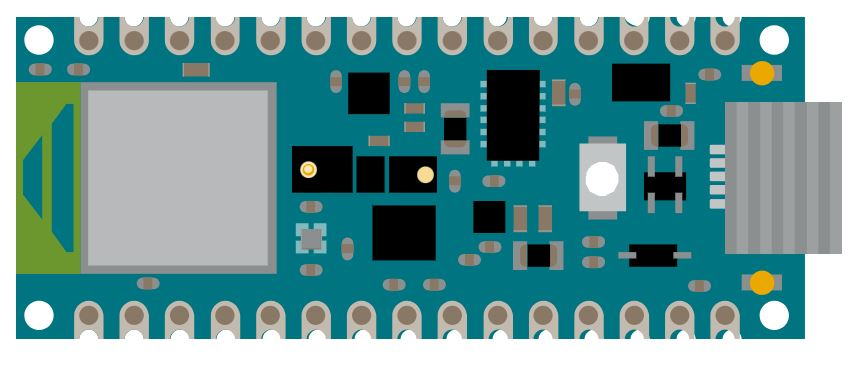
\includegraphics{Arduino/Nano33BLE/Nano33BLESense}};

  \fill[gray, opacity=0.7] (-6,-2.4) rectangle (6,2.4);

  \coordinate (A) at (\LowerLeftX,\LowerLeftY);
  \coordinate (B) at (\UpperRightX,\UpperRightY);    
  \begin{scope}
    \clip (A) rectangle (B);
    
    \node at (0,0) (Board) {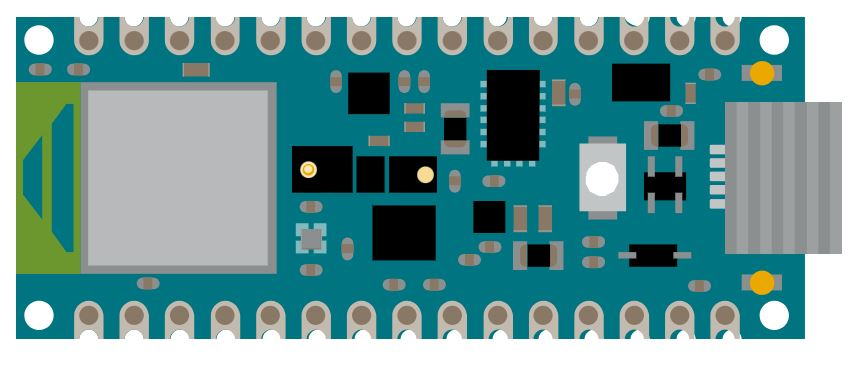
\includegraphics{Arduino/Nano33BLE/Nano33BLESense}};
    
  \end{scope}
  \draw[yellow,line width=2pt] (A)  rectangle (B);

}

%%%%%%%%%%%%%%%%%%%%%%%%%%%%%%
%
% $Autor: Wingss $
% $Datum: 2020-10-12 $
% $Pfad: \Documents\200526CUDA\report\Allgemein\acronyms.tex $
% $Version: 1 $
%
%
%%%%%%%%%%%%%%%%%%%%%%%%%%%%%%

% Automatisches erstellen und referenzieren eines Abkürzungsverzeichnisses
%\usepackage[tooltip]{acro}
\usepackage{acro}
%\usepackage{acronym} nicht in Verwendung; hier erwähnt, weil immer Verwechslungen auftreten.



%\acsetup{
%%    list-type    = table ,
%    list-name    = Akronyme,
%    list-style   = longtable ,
%    list-heading = chapter*, % Kapitel ohne Nummerierung
%%    list-table-width = \textwidth-4\tabcolsep-6em,
%%    page-ref = dotfill , % <<< neue Instanz verwenden
%    list-short-format ={\bfseries}, % Abkürzungen in fetter Serifenschrift im Verzeichnis
%    first-long-format = {\itshape}, % Erste Lange Ausführung der Abkürzung kursiv gestellt
%}

% muss für Akronyme \ac statt see verwendet werden.
%\newcommand{\Siehe}{
%	\ifdefined\isGerman
%	\emph{siehe}
%	\else
%	\ifdefined\isEnglish
%	\emph{see}
%	\else
%	\emph{siehe}
%	\fi
%	\fi
%}


%%%%%%%%%%%%%%%%%%%%%%%%%%%%%%%%%%%%%%%%%%%%%%%%%%%%%
% A
%%%%%%%%%%%%%%%%%%%%%%%%%%%%%%%%%%%%%%%%%%%%%%%%%%%%%




\DeclareAcronym{adc}{
	short = ADC\index{ADC}, 
	long  = Analog to Digital Converter\index{Analog to Digital Converter!\Siehe ADC},
}

\DeclareAcronym{ai}{
    short = AI\index{AI}, 
    long  = Artificial Intelligence\index{Artificial Intelligence!\Siehe {AI}},
}

\DeclareAcronym{aop}{
    short = AOP\index{AOP}, 
    long  = Acoustic Overload Point\index{Acoustic Overload Point!\Siehe AOP},
}

\DeclareAcronym{ap}{
	short = AP\index{AP}, 
	long  = Average Precision\index{Average Precision!\Siehe {AP}},
}

\DeclareAcronym{api}{
    short = API\index{API}, 
    long  = Application Programming Interface\index{Application Programming Interface!\Siehe {API}},
}

\DeclareAcronym{ARM}{
	short = ARM\index{ARM}, 
	long  = Advanced RISC Machine\index{Advanced RISC Machine!\Siehe ARM},
}


%%%%%%%%%%%%%%%%%%%%%%%%%%%%%%%%%%%%%%%%%%%%%%%%%%%%%
% B
%%%%%%%%%%%%%%%%%%%%%%%%%%%%%%%%%%%%%%%%%%%%%%%%%%%%%

\DeclareAcronym{ble}{
    short = BLE\index{BLE},
    long  = Bluetooth Low Energy\index{Bluetooth Low Energy!\Siehe BLE},
}

\DeclareAcronym{bs}{
    short = BS\index{BS}, 
    long  = Batch-Size\index{Batch-Size!\Siehe {BS}},
}

%%%%%%%%%%%%%%%%%%%%%%%%%%%%%%%%%%%%%%%%%%%%%%%%%%%%%
% C
%%%%%%%%%%%%%%%%%%%%%%%%%%%%%%%%%%%%%%%%%%%%%%%%%%%%%

\DeclareAcronym{cad}{
    short = CAD\index{CAD},
    long  = Computer Aided Design\index{Computer Aided Design!\Siehe CAD},
}

\DeclareAcronym{cci}{
    short = CCI\index{CCI},
    long  = Camera Control Interface\index{Camera Control Interface!\Siehe {CCI}},
}

\DeclareAcronym{cli}{
	short = CLI\index{CLI},
%	long  = \TRANS{Kommandozeilenschnitte}{Command Line Interface}\index{\TRANS{Kommandozeilenschnitte}{Command Line Interface}!\Siehe {CCI}},
	long  = Command Line Interface\index{Command Line Interface!\Siehe {CCI}},
}

\DeclareAcronym{csi}{
  short = CSI\index{CSI},
  long  = Camera Serial Interface\index{Camera Serial Interface!\Siehe {CSI}},
}
  
\DeclareAcronym{cg}{
    short = Cg, 
    long = C for graphics,
}

\DeclareAcronym{cifar}{
    short = CIFAR\index{Datensatz!CIFAR} ,
    long  = Canadian Institute For Advanced Research\index{Canadian Institute For Advanced Research!\Siehe {CIFAR!\Siehe {Datensatz}}},
}

\DeclareAcronym{cnc}{
	short = CNC\index{CNN} ,
	long  = Computerized Numerical Control\index{Computerized Numerical Control!\Siehe {CNN}} ,
}

\DeclareAcronym{cnn}{
    short = CNN\index{CNN} ,
    long  = Convolutional Neural Network\index{Convolutional Neural Network!\Siehe {CNN}} ,
}

\DeclareAcronym{coco}{
  short = COCO\index{COCO},
  long  = Common Objects in Context\index{Common Objects in Context!\Siehe {COCO}}
}

\DeclareAcronym{cpu}{
    short = CPU\index{CPU} ,
    long  = Central Processing Unit\index{Central Processing Unit!\Siehe {CPU}} ,
}


\DeclareAcronym{csp}{
	short = CSP\index{CSP} ,
	long  = Cross Stage Partial Network\index{Cross Stage Partial Network!\Siehe {CSP}} ,
}

\DeclareAcronym{cuda}{
    short = CUDA\index{CUDA} ,
	long  = Compute Unified Device Architecture\index{Compute Unified Device Architecture!\Siehe {CUDA}} ,
}

\DeclareAcronym{cudnn}{
	short = cuDNN\index{cuDNN} ,
	long  = NVIDIA CUDA Deep Neural Network Library\index{NVIDIA CUDA Deep Neural Network Library!\Siehe {cuDNN}} ,
}

%%%%%%%%%%%%%%%%%%%%%%%%%%%%%%%%%%%%%%%%%%%%%%%%%%%%%
% D
%%%%%%%%%%%%%%%%%%%%%%%%%%%%%%%%%%%%%%%%%%%%%%%%%%%%%

\DeclareAcronym{dac}{
	short = DAC\index{DAC}, 
	long  = Digital to Analog Converter\index{Digital to Analog Converter!\Siehe DAC},
}

\DeclareAcronym{diy}{
    short = DIY\index{DIY}, 
    long  = Do It Yourself\index{Do It Yourself!\Siehe {DIY}},
}

\DeclareAcronym{dll}{
    short = DLL ,
    long  = Dynamic Link Library,
    long-plural-form = Dynamic Link Libraries,
}

\DeclareAcronym{dnn}{
    short = DNN ,
    long  = Deep Neural Network ,
}

%%%%%%%%%%%%%%%%%%%%%%%%%%%%%%%%%%%%%%%%%%%%%%%%%%%%%
% E
%%%%%%%%%%%%%%%%%%%%%%%%%%%%%%%%%%%%%%%%%%%%%%%%%%%%%

\DeclareAcronym{ean}{
    short = EAN\index{EAN},
    long  = European Article Number\index{European Article Number!\see EAN},
}

\DeclareAcronym{esp32}{
    short = ESP32\index{ESP32},
    long  = Espressif32\index{Espressif32!\see ESP32},
}

\DeclareAcronym{esp32cam}{
    short = ESP32-CAM\index{ESP32-CAM},
    long  = Espressif32 Camera Module\index{Espressif32 Camera Module!\see ESP32-CAM},
}

\DeclareAcronym{espidf}{
    short = ESP-IDF\index{ESP-IDF},
    long = Espressif IoT Development Framework\index{Espressif IoT Development Framework!\see ESP-IDF},
}

%%%%%%%%%%%%%%%%%%%%%%%%%%%%%%%%%%%%%%%%%%%%%%%%%%%%%
% F
%%%%%%%%%%%%%%%%%%%%%%%%%%%%%%%%%%%%%%%%%%%%%%%%%%%%%

\DeclareAcronym{fp32}{
    short = FP32, 
    long  = Floating Point 32-bit,
}

\DeclareAcronym{flops}{
    short = Flops, 
    long  = Floating Point Operations per Second - Gleitkomma­operationen pro Sekunde,
}


\DeclareAcronym{fp16}{
    short = FP16, 
    long = Floating Point 16-bit,
}

\DeclareAcronym{fpga}{
  short = FPGA,
  long  = Field-Programmable Gate Array,
}

\DeclareAcronym{fps}{
    short = fps,
    long  = frames per second,
}


%%%%%%%%%%%%%%%%%%%%%%%%%%%%%%%%%%%%%%%%%%%%%%%%%%%%%
% G
%%%%%%%%%%%%%%%%%%%%%%%%%%%%%%%%%%%%%%%%%%%%%%%%%%%%%

\DeclareAcronym{gpio}{
  short = GPIO\index{GPIO},
  long  = General Purpose Input Output\index{General Purpose Input Output!\Siehe GPIO},
}

\DeclareAcronym{gpgpu}{
    short = GPGPU ,
    long  = General Purpose Computation on Graphics Processing Unit\index{General Purpose Computation on Graphics Processing Unit!\Siehe GPGPU} ,
}

\DeclareAcronym{gpu}{
    short = GPU\index{GPU} ,
    long  = Graphics Processing Unit\index{Graphics Processing Unit!\Siehe GPU} ,
}

%%%%%%%%%%%%%%%%%%%%%%%%%%%%%%%%%%%%%%%%%%%%%%%%%%%%%
% H
%%%%%%%%%%%%%%%%%%%%%%%%%%%%%%%%%%%%%%%%%%%%%%%%%%%%%

\DeclareAcronym{hdmi}{
  short = HDMI\index{HDMI},
  long  = High Definition Multimedia Interface\index{High Definition Multimedia Interface!\Siehe {HDMI}},
}

\DeclareAcronym{hw}{
    short = HW\index{HW}, 
    long  = Hardware\index{Hardware!\Siehe {HW}},
}

%%%%%%%%%%%%%%%%%%%%%%%%%%%%%%%%%%%%%%%%%%%%%%%%%%%%%
% I
%%%%%%%%%%%%%%%%%%%%%%%%%%%%%%%%%%%%%%%%%%%%%%%%%%%%%


\DeclareAcronym{i2c}{
    short = I\textsuperscript{2}C\index{I\textsuperscript{2}C},
    long  = Inter-Integrated Circuit\index{Inter-Integrated Circuit!\Siehe I\textsuperscript{2}C},
}    

\DeclareAcronym{i2s}{
    short = I\textsuperscript{2}S\index{I\textsuperscript{2}S},
    long  = Inter-IC Sound\index{Inter-IC Sound!\Siehe I\textsuperscript{2}S},
}    

\DeclareAcronym{ide}{
	short = IDE\index{IDE} ,
	long  = Integrated Development Environment\index{Integrated Development Environment!\Siehe IDE},
}

\DeclareAcronym{imu}{
    short = IMU\index{IMU} ,
    long  = \TRANS{Inertialmesseinheit}{Inertial Measurement Unit}\index{\TRANS{Inertialmesseinheit}{Inertial Measurement Unit}!\Siehe IMU},
}


\DeclareAcronym{int8}{
    short = INT8, 
    long = Integer 8-bit,
}

\DeclareAcronym{iot}{
    short = IoT ,
    long  = Internet of Things,
}

\DeclareAcronym{ir}{
    short = IR ,
    long  = Infrarot,
}

%%%%%%%%%%%%%%%%%%%%%%%%%%%%%%%%%%%%%%%%%%%%%%%%%%%%%
% J
%%%%%%%%%%%%%%%%%%%%%%%%%%%%%%%%%%%%%%%%%%%%%%%%%%%%%

%%%%%%%%%%%%%%%%%%%%%%%%%%%%%%%%%%%%%%%%%%%%%%%%%%%%%
% K
%%%%%%%%%%%%%%%%%%%%%%%%%%%%%%%%%%%%%%%%%%%%%%%%%%%%%

\DeclareAcronym{kdd}{
    short = KDD\index{KDD} ,
    long  = Knowledge Discovery in Databases\index{Knowledge Discovery in Databases!\Siehe KDD},
}

\DeclareAcronym{ki}{
    short = KI, 
    long  = Künstliche Intelligenz,
}

\DeclareAcronym{knn}{
    short = KNN, 
    long  = Künstliches Neuronales Netz,
}

%%%%%%%%%%%%%%%%%%%%%%%%%%%%%%%%%%%%%%%%%%%%%%%%%%%%%
% L
%%%%%%%%%%%%%%%%%%%%%%%%%%%%%%%%%%%%%%%%%%%%%%%%%%%%%

\DeclareAcronym{led}{
    short = LED\index{LED}, 
    long  = Light Emitting Diode\index{Light Emitting Diode!\Siehe {LED}},
}

%%%%%%%%%%%%%%%%%%%%%%%%%%%%%%%%%%%%%%%%%%%%%%%%%%%%%
% M
%%%%%%%%%%%%%%%%%%%%%%%%%%%%%%%%%%%%%%%%%%%%%%%%%%%%%

\DeclareAcronym{mcd}{
    short = mcd\index{mcd}, 
    long  = Millicandela\index{Millicandela!\Siehe {mcd}},
}

\DeclareAcronym{mimd}{
    short = MIMD \index{MIND},
    long  = Multiple-Instruction Multiple-Data\index{Multiple-Instruction Multiple-Data!\Siehe MIMD} ,
}

\DeclareAcronym{ml}{
    short = ML\index{ML}, 
    long  = Machine Learning\index{Machine Learning!\Siehe {ML}},
}

\DeclareAcronym{mp}{
    short = MP\index{MP},
    long = Megapixels\index{Megapixels!\see MP},
}


%%%%%%%%%%%%%%%%%%%%%%%%%%%%%%%%%%%%%%%%%%%%%%%%%%%%%
% N
%%%%%%%%%%%%%%%%%%%%%%%%%%%%%%%%%%%%%%%%%%%%%%%%%%%%%

\DeclareAcronym{nn}{
    short = NN, 
    long  = Neuronales Netz,
}

\DeclareAcronym{NumPy}{
    short = NumPy\index{NumPy}, 
    long  = Numerical Python\index{Numerical Python\!\Siehe {NumPy}},
}

%%%%%%%%%%%%%%%%%%%%%%%%%%%%%%%%%%%%%%%%%%%%%%%%%%%%%
% O
%%%%%%%%%%%%%%%%%%%%%%%%%%%%%%%%%%%%%%%%%%%%%%%%%%%%%

\DeclareAcronym{ocr}{
    short = OCR\index{OCR}, 
    long  = Optical Character Recognition\index{Optical Character Recognition\!\Siehe {OCR}},
}

\DeclareAcronym{opencl}{
    short = OpenCL\index{OpenCL}, 
    long  = Open Computing Language\index{Open Computing Language!\Siehe OpenCL},
}

\DeclareAcronym{oled}{
    short = OLED\index{OLED}, 
    long  = Organic Light Emitting Diode\index{Organic Light Emitting Diode!\Siehe {OLED}},
}

\DeclareAcronym{ov2640}{
    short = OV2640\index{OV2640},
    long  = OmniVision 2640 \index{OmniVision 2640!\see OV2640},
}


%%%%%%%%%%%%%%%%%%%%%%%%%%%%%%%%%%%%%%%%%%%%%%%%%%%%%
% P
%%%%%%%%%%%%%%%%%%%%%%%%%%%%%%%%%%%%%%%%%%%%%%%%%%%%%

\DeclareAcronym{pan}{
	short = PAN\index{PAN} ,
	long  = Path Aggregation Network\index{Path Aggregation Network!\Siehe PAN} ,
}

\DeclareAcronym{pc}{
    short = PC\index{PC}, 
    long  = Personal Computer\index{Personal Computer!\Siehe {PC}},
}

\DeclareAcronym{pcb}{
    short = PCB\index{PCB},
    long = Printed Circuit Board\index{Printed Circuit Board!\see PCB},
}

\DeclareAcronym{PIL}{
    short = PIL\index{PIL}, 
    long  = Python Imaging Library\index{Python Imaging Library\!\Siehe {PIL}},
}

\DeclareAcronym{pdm}{
    short = PDM\index{PDM} ,
    long  = Pulse Density Modulation\index{Pulse Density Modulation!\Siehe PDM} ,
}

\DeclareAcronym{pla}{
    short = PLA\index{PLA},
    long  = Polylactic Acid\index{Polylactic Acid!\Siehe PLA},
}

\DeclareAcronym{ppa}{
    short = PPA\index{PPa}, 
    long  = Personal Package Archive\index{Personal Package Archive!\Siehe PPA},
}

\DeclareAcronym{pip}{
	short = pip\index{pip} ,
	long  = pip installs packages\index{pip installs packages!\Siehe pip} ,
}

\DeclareAcronym{pypi}{
	short = PyPi\index{PyPi} ,
	long  = Python Package Index\index{Python Package Index!\Siehe PyPi} ,
}

\DeclareAcronym{pwm}{
    short = PWM\index{PWM Signal} ,
    long  = Pulse with Modulation\index{Pulse with Modulation!\Siehe PWM Signal} ,
}

%%%%%%%%%%%%%%%%%%%%%%%%%%%%%%%%%%%%%%%%%%%%%%%%%%%%%
% Q
%%%%%%%%%%%%%%%%%%%%%%%%%%%%%%%%%%%%%%%%%%%%%%%%%%%%%


%%%%%%%%%%%%%%%%%%%%%%%%%%%%%%%%%%%%%%%%%%%%%%%%%%%%%
% R
%%%%%%%%%%%%%%%%%%%%%%%%%%%%%%%%%%%%%%%%%%%%%%%%%%%%%

\DeclareAcronym{ram}{
	short = RAM\index{RAM} ,
	long  = Random Access Memory\index{Random Access Memory! \Siehe RAM},
}

\DeclareAcronym{relu}{
    short = ReLu\index{ReLu}, 
    long  = Rectified Linear Unit\index{Rectified Linear Unit!\Siehe ReLu},
}

\DeclareAcronym{resnets}{
    short = ResNet\index{ResNet},
    long =  Residual Neural Network\index{Residual Neural Network!\Siehe ResNet},
}    


\DeclareAcronym{rle}{
    short = RLE\index{RLE},
    long  = Run-Length Encoding\index{Run-Length Encoding},
}

\DeclareAcronym{rgb}{
  short = RGB,
  long  = Rot-Grün-Blau}

\DeclareAcronym{roi}{
	short = ROI\index{Region of Interest},
	long  = Region of Interest\index{Region of Interest}
}

\DeclareAcronym{rtos}{
    short = RTOS\index{RTOS}, 
    long  = Real Time Operating System\index{Real Time Operating System!\see RTOS},
}

\DeclareAcronym{rpc}{
	short = RPC\index{RPC}, 
	long  = Remote call procedure\index{Remote call procedure!\Siehe RPC},
}

\DeclareAcronym{RTOS}{
	short = RTOS\index{RTOS}, 
	long  = Real Time Operating System\index{Real Time Operating System!\Siehe RTOS},
}


%%%%%%%%%%%%%%%%%%%%%%%%%%%%%%%%%%%%%%%%%%%%%%%%%%%%%
% S
%%%%%%%%%%%%%%%%%%%%%%%%%%%%%%%%%%%%%%%%%%%%%%%%%%%%%

\DeclareAcronym{sd}{
  short = SD\index{SD},
  long  = Secure Digital\index{Secure Digital!\Siehe SD},
}

\DeclareAcronym{sda}{
    short = SDA\index{SDA},
    long  = Serial Data\index{Serial Data!\Siehe SDA},
}    

\DeclareAcronym{sd-1}{
    short = SD-1\index{Datensatz!NIST~Special~Database~1},
    long  = NIST Special Database~1\index{NIST Special Database 1!\Siehe Datensatz},
}    

\DeclareAcronym{sd-3}{
    short = SD-3\index{Datensatz!NIST Special Database 3},
    long  = NIST Special Database 3\index{NIST Special Database 3!\Siehe Datensatz},
}    


\DeclareAcronym{scl}{
    short = SCL\index{SCL},
    long  = Serial Clock\index{Serial Clock!\Siehe SCL},
}    

\DeclareAcronym{ssh}{
    short = SSH\index{SSH},
    long  = Secure Shell\index{Secure Shell!\Siehe SSH},
}

\DeclareAcronym{spi}{
    short = SPI\index{SPI},
    long  = Serial Peripheral Interface\index{Serial Peripheral Interface!\Siehe SPI},
}
 
 
\DeclareAcronym{sbc}{
    short = SBC\index{SBC} ,
    long  = Single-Board-Computer\index{Single-Board-Computer!\Siehe SBC} ,
}

\DeclareAcronym{simd}{
	short = SIMD\index{SIMD} ,
	long  = Single-Instruction Multiple-Data\index{Single-Instruction Multiple-Data!\Siehe SIMD} ,
}

\DeclareAcronym{sm}{
	short = SM\index{SM} ,
	long  = Streaming Multiprocessor\index{Streaming Multiprocessor!\Siehe SM} ,
}

\DeclareAcronym{sp}{
	short = SP\index{SP} ,
	long  = Streaming Processor\index{Streaming Processor!\Siehe SP} ,
}

\DeclareAcronym{spp}{
	short = SP\index{SP} ,
	long  = Streaming Processor\index{Streaming Processor!\Siehe SP} ,
}

\DeclareAcronym{sps}{
    short = SPS\index{SPS} ,
    long  = Speicherprogrammierbare Steuerung\index{Speicherprogrammierbare Steuerung!\Siehe SPS} ,
}

\DeclareAcronym{sram}{
    short = SRAM\index{SRAM},
    long  = Static Random Access Memory\index{Static Random Access Memory!\Siehe SRAM},
}   

\DeclareAcronym{sw}{
    short = SW\index{SW}, 
    long  = Software\index{Software!\Siehe {SW}},
}

%%%%%%%%%%%%%%%%%%%%%%%%%%%%%%%%%%%%%%%%%%%%%%%%%%%%%
% T
%%%%%%%%%%%%%%%%%%%%%%%%%%%%%%%%%%%%%%%%%%%%%%%%%%%%%

\DeclareAcronym{tf}{
    short = tf\index{tf}, 
    long  = TensorFlow\index{TensorFlow\!\Siehe {tf}},
}

\DeclareAcronym{tfcard}{
    short = TF Card\index{TF},
    long = TransFlash Card\index{TransFlash Card!\see TF},
}

\DeclareAcronym{tfl}{
    short = TFLite\index{TFLite}, 
    long  = TensorFlow-Lite\index{TensorFlow-Lite\!\Siehe {TFLite}},
}

\DeclareAcronym{tpu}{
	short = TPU\index{TPU}, 
	long  = Tensor Processing Unit\index{Tensor Processing Unit!\Siehe TPU},
}

%%%%%%%%%%%%%%%%%%%%%%%%%%%%%%%%%%%%%%%%%%%%%%%%%%%%%
% U
%%%%%%%%%%%%%%%%%%%%%%%%%%%%%%%%%%%%%%%%%%%%%%%%%%%%%


\DeclareAcronym{uart}{
    short = UART\index{UART}, 
    long  = Universal Asynchronous Receiver Transmitter\index{Universal Asynchronous Receiver Transmitter!\Siehe UART},
}

\DeclareAcronym{ui}{
	short = UI\index{UI},
	long = user interface\index{user interface!\Siehe UI},
}

\DeclareAcronym{uma}{
  short = UMA\index{UMA}, 
  long  = Unified Memory Architecture\index{Unified Memory Architecture!\Siehe UMA},
}

\DeclareAcronym{usb}{
    short = USB\index{USB}, 
    long  = Universal Serial Bus\index{Universal Serial Bus!\Siehe USB},
}

%%%%%%%%%%%%%%%%%%%%%%%%%%%%%%%%%%%%%%%%%%%%%%%%%%%%%
% V
%%%%%%%%%%%%%%%%%%%%%%%%%%%%%%%%%%%%%%%%%%%%%%%%%%%%%

\DeclareAcronym{venv}{
    short = VENV\index{VENV} ,
    long  = Virtual Environment\index{Virtual Environment!\Siehe VENV} ,
}

\DeclareAcronym{vin}{
    short = VIN\index{VIN}, 
    long  = Voltage Input\index{Voltage Input!\Siehe VIN},
}

\DeclareAcronym{vpu}{
  short = VPU\index{VPU},
  long  = Video Processing Unit\index{Video Processing Unit!\Siehe VPU},
}

 
\DeclareAcronym{vm}{
	short = VM\index{VM},
	long  = Virtual Machine\index{Virtual Machine!\Siehe VM},
}


\DeclareAcronym{vnc}{
	short = VNC\index{VNC} ,
	long  = Virtual Network Computing\index{Virtual Network Computing!\Siehe VNC} ,
}

\DeclareAcronym{vscode}{
    short = VSCode\index{VSCode}, 
    long  = Visual Studio Code\index{Visual Studio Code!\Siehe {VSCode}},
}

  
%%%%%%%%%%%%%%%%%%%%%%%%%%%%%%%%%%%%%%%%%%%%%%%%%%%%%
% W
%%%%%%%%%%%%%%%%%%%%%%%%%%%%%%%%%%%%%%%%%%%%%%%%%%%%%

\DeclareAcronym{wifi}{
    short = WiFi\index{WiFi},
    long = Wireless Fidelity\index{Wireless Fidelity!\see WiFi},
}

%%%%%%%%%%%%%%%%%%%%%%%%%%%%%%%%%%%%%%%%%%%%%%%%%%%%%
% X
%%%%%%%%%%%%%%%%%%%%%%%%%%%%%%%%%%%%%%%%%%%%%%%%%%%%%


%%%%%%%%%%%%%%%%%%%%%%%%%%%%%%%%%%%%%%%%%%%%%%%%%%%%%
% Y
%%%%%%%%%%%%%%%%%%%%%%%%%%%%%%%%%%%%%%%%%%%%%%%%%%%%%


\DeclareAcronym{yolo}{
	short = YOLO\index{YOLO},
	long  = You Only Look Once\index{You Only Look Once!\Siehe YOLO},
}

%%%%%%%%%%%%%%%%%%%%%%%%%%%%%%%%%%%%%%%%%%%%%%%%%%%%%
% Z
%%%%%%%%%%%%%%%%%%%%%%%%%%%%%%%%%%%%%%%%%%%%%%%%%%%%%



%%%%%%%%%%%%%%%%%%%%%%%%%%%%%%
%
% $Autor: Wings $
% $Datum: 2019-12-09 11:50:02Z $
% $Pfad: komponenten/Bilderkennung/Produktspezifikation/CorelTPU/TPU/Allgemein/Hyphenations.tex $
% $Version: 1766 $
%
%
%%%%%%%%%%%%%%%%%%%%%%%%%%%%%%


\usepackage[babel]{microtype}
\hyphenchar\font=\string"7F

\hyphenation{De-na-vit-Har-ten-berg-Kon-ven-tion}
\hyphenation{De-na-vit-Har-ten-berg-Dar-stel-lung}
\hyphenation{De-na-vit-Har-ten-berg-Pa-ra-me-ter}
\hyphenation{Fließ-kom-ma-a-ri-thme-tik}
\hyphenation{ent-we-der}%

\bibliography{../../MLbib/Jetson} 



%\InputLanguage


\begin{document}


%%%%%%%%%%%%%%%%%%%%%%%%
%
% $Autor: Wings $
% $Datum: 2020-01-29 07:55:27Z $
% $Pfad: komponenten/Bilderkennung/Produktspezifikation/IntelNCS2/Inhalt/Titelseite.tex $
% $Version: 1785 $
%
%%%%%%%%%%%%%%%%%%%%%%%%


%%%%%%%%%%%%%%%%%%%%%%%%
%
% $Autor: Wings $
% $Datum: 2019-12-09 11:47:41Z $
% $Pfad: komponenten/Bilderkennung/Produktspezifikation/JetsonNano/Inhalt/Titelseite.tex $
% $Version: 1765 $
%
%%%%%%%%%%%%%%%%%%%%%%%%



\definecolor{airforceblue}{rgb}{0.36, 0.54, 0.66}

\definecolor{ballblue}{rgb}{0.13, 0.67, 0.8}

\definecolor{blue(munsell)}{rgb}{0.0, 0.5, 0.69}

\definecolor{blue(ncs)}{rgb}{0.0, 0.53, 0.74}

\definecolor{bondiblue}{rgb}{0.0, 0.58, 0.71}

\definecolor{cerulean}{rgb}{0.0, 0.48, 0.65}

\definecolor{pink}{rgb}{0.5882, 0, 0.4314}

\begin{titlepage}
	
	{\hspace{-50mm}\vspace{-10mm}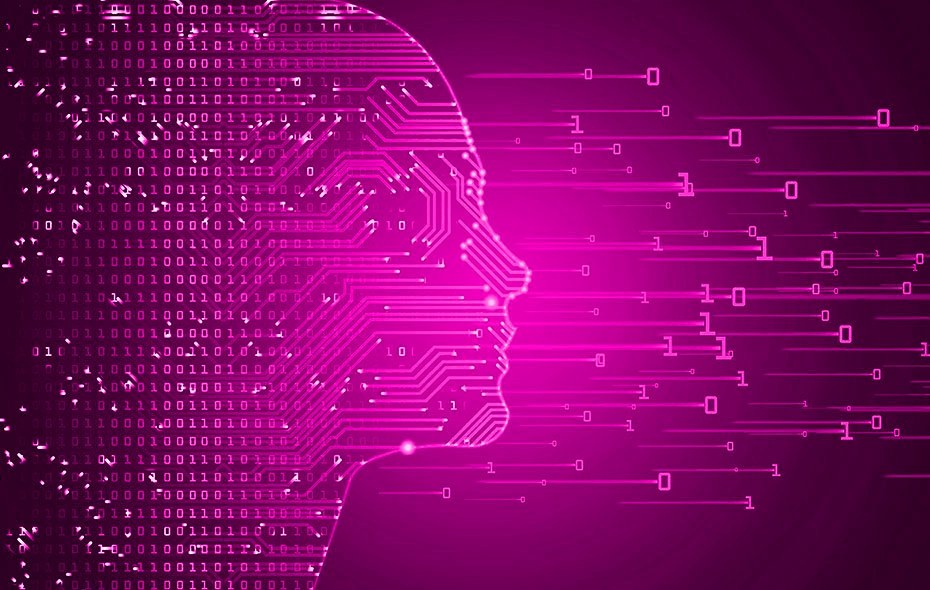
\includegraphics[width=220mm,height=80mm]{Allgemein/LogoDataSciencePink.jpg}};
	
	\vspace{20mm}
	
	
	
	{\hspace{-50mm}%\vspace{-30mm}
		\begin{tikzpicture}
			\draw[pink,fill] (0,-1) -- (0,2) -- (80,2) -- (80,-1) -- cycle;
			
			
			\node[black,right] (Name) at (3,3) {\Huge \textsf{Elmar Wings}};
			\node[white,right] (Title) at (3,1) {\Huge \textsf{\TRANS{Künstliche Intelligenz mit dem Arduino Portenta H7}{Artificial Intelligence with an Arduino Portenta H7}}};
			\node[white,right] (Title) at (3,0) {\LARGE \textsf{\TRANS{Echtzeit-Objekterkennung mit dem Vision Shield}{Realtime Object Detection with a Vision Shield}}};
			%  \node (logo) at (0,10) {\hspace{-50mm}\vspace{-10mm}\includegraphics[width=220mm,height=80mm]{Allgemein/LogoDataScience.jpg}};
		\end{tikzpicture}
	}
	
	%
	%\begin{minipage}[X]{0.8\textwidth}
	%\begin{tikzpicture}
	%  \draw[black] (0,0) -- (0,10) -- (10,20) -- (10,0) -- cycle;
	%  \node (logo) at (0,10) {\hspace{-50mm}\vspace{-10mm}\includegraphics[width=220mm,height=80mm]{Allgemein/LogoDataScience.jpg}};
	%\end{tikzpicture}
	%\end{minipage}
	%\includegraphics[width=1.4\textwidth]{Allgemein/LogoDataScience.jpg}\hfill
	
	\vfill
	\begin{tabular}{l}
		{$ $Version: 1765 $ $}\\
		\today\\
	\end{tabular}		
	%	\hfill
\includegraphics[width=0.4\textwidth]{Images/Technik.jpg} \par\vspace{1cm}
	
	
	
\end{titlepage}

\newpage



\tableofcontents
\cleardoublepage

\listoffigures
\cleardoublepage

%\addcontentsline{toc}{chapter}{\TRANS{Liste der Programme}{List of Listings}}
%\lstlistoflistings
\listofcodes
\cleardoublepage

\InputLanguage{../Contents/General/}{Acronymlist}
\cleardoublepage


%\Ausblenden
{
\TRANS{\part{Maschinelles Lernen}}{\part{Machine Learning}}

\InputLanguage{../contents/General/}{ki}

\InputLanguage{../contents/General/}{Adversarial}

\InputLanguage{../contents/General/}{kdd} 

\InputLanguage{../contents/General/}{NeuralNetwork} 

\InputLanguage{../contents/General/}{Images}

\InputLanguage{../contents/General/}{cnn} 

\InputLanguage{../contents/General/}{Databases}

%%%%%%%%%%%%%%%    
\section{Datenbanken}

\InputLanguage{../contents/General/}{mnist}

\InputLanguage{../contents/General/}{cifar}

\InputLanguage{../contents/General/}{iris}

\InputLanguage{../contents/General/}{coco}

\InputLanguage{../contents/General/}{ImageNet}

\InputLanguage{../contents/General/}{VisualWakeWords}

\InputLanguage{../contents/General/}{UTKFace}

\InputLanguage{../contents/General/}{models}

%%%%%%
%
% $Autor: Wings $
% $Datum: 2021-05-14 $
% $Pfad: GitLab/MLEdgeComputer/ $
% $Dateiname: FaceNet
% $Version: 4620 $
%
%%%%%%

%todo Hier ist viel zu tun: Keine Quellen
% nicht ausführlich genug

\section{FaceNet}

\cite{Schroff:2015}

%facenet-120\cite{Schroff:2015}

FaceNet lernt eine Abbildung von Gesichtsbildern auf einem kompakten euklidischen Raum, in dem Abstände direkt einem Maß für die Ähnlichkeit von Gesichtern entsprechen. Sobald dies geschehen ist, sind Aufgaben wie Gesichtserkennung, -verifizierung und -clusterung mit Standardtechniken (unter Verwendung der FaceNet-Einbettungen als Merkmale) einfach zu erledigen.
Verwendet ein Deep CNN, das trainiert wird, um die Einbettung selbst zu optimieren, anstatt die Ausgabe einer dazwischenliegenden Engpassschicht zu verwenden. Das Training erfolgt mit Triplets: ein Bild eines Gesichts ("Anker"), ein weiteres Bild desselben Gesichts ("positives Exemplar") und ein Bild eines anderen Gesichts ("negatives Exemplar"). Der Hauptvorteil liegt in der Repräsentationseffizienz: Mit nur 128 Byte pro Gesicht kann eine Spitzenleistung erzielt werden (Rekordgenauigkeit von 99,63 \% bei LFW, 95,12 \% bei Youtube Faces DB).

siehe \url{../../MLbib/CNN/class10_FaceNet.pdf}



FaceNet ist ein tiefes Faltungsneuronales Netzwerk, das von Google-Forschern entwickelt und um 2015 eingeführt wurde, um die Hürden bei der Gesichtserkennung und -verifizierung effektiv zu lösen. Der FaceNet-Algorithmus transformiert das Gesichtsbild in einen 128-dimensionalen euklidischen Raum, ähnlich wie beim Word Embedding[9]. Das so erstellte FaceNet-Modell wird auf Triplett-Verlust trainiert, um die Ähnlichkeiten und Unterschiede auf dem bereitgestellten Bilddatensatz zu erfassen. Die vom Modell erzeugten Einbettungen mit 128 Dimensionen können verwendet werden, um Gesichter auf sehr effektive und präzise Weise zu clustern. Durch die Verwendung von FaceNet-Embeddings als Merkmalsvektoren könnten nach der Erstellung des Vektorraums Funktionalitäten wie Gesichtserkennung und -verifikation implementiert werden[10]. Kurz gesagt, die Abstände für die ähnlichen Bilder würden viel näher sein als die zufälligen nicht ähnlichen Bilder. Die allgemeine Blockdarstellung des FaceNet-Ansatzes der Gesichtserkennung ist in Abb.1 dargestellt.

siehe \url{../../MLbib/CNN/10.1109ICACCS.2019.8728466.pdf}

Eingabeformat? Farben? Pixelauflösung?
%%%%%%%%%%%%%%%    

\InputLanguage{../contents/General/}{Frameworks}

\InputLanguage{../contents/General/}{FaceDetection}
}

%\Ausblenden
{
    
    \part{Tools}
    
    \InputLanguage{../contents/General/}{ArduinoIDE}
    
    \InputLanguage{../contents/PortentaH7/}{ArduinoIDEFirstSteps}
    
    %%%%%%%%%%%%%%%
%
% $Autor: Wings $
% $Datum: 2020-01-29 07:55:27Z $
% $Pfad: General/ArduinoCLI.tex
% $Version: 1785 $
%
%
%%%%%%%%%%%%%%%


%@online{ArduinoCLI:2018,
%  publisher = Arduino,
%  year      = 2018,
%  title     = {Arduino CLI 0.33},
%  url = {https://arduino.github.io/arduino-cli/0.33/commands/arduino-cli/}
%}

\chapter{Kammandozeileninterpreter (CLI)}

\textcolor{red}{Quellen für die Bilder fehlen!}

\Mynote{Erklärung von Kammandos in den Anhang}

Seit 2018 bietet die Firma Arduino auch einen Kommandozeileninterpreter an. \cite{ArduinoCLI:2018} Die Web-Version der Entwicklungsumgebung verwendet diese Schnittstelle. Das heißt, alle Funktionalitäten, die die Entwicklungsumgebung zur Verfügung stellt, stehen hier auch zur Verfügung. So kann unter Windows, MacOS und Linux \cite{ArduinoCLI:2022}. Die Entwicklung mit Hilfe des Kommandozeileninterpreters ermöglicht es, wenn konsequent mit Hilfe von Batch-Dateien gearbeitet wird, qualitätssichernde Maßnahmen gezielt durchzuführen. So kann die Konfiguration der Entwicklungsumgebung gesichert und nachvollziehbar wiederholt werden. 


Der Quellcode  kann frei genutzt werden, allerdings muss man bei einer gewerblichen Nutzung eine Lizenz bei der Firma anfragen \cite{ArduinoCLIGit:2022}. Eine ausführliche Dokumentation wird zur Verfügung gestellt. \cite{ArduinoCLIIntro:2020,ArduinoCLIDoc:2022}

Bei der Entwicklung der \ac{cli} stehen drei Aspekte im Fokus. 

\begin{enumerate}
  \item Einerseits ermöglicht die Schnittstelle die Einbettung der Entwicklung in die gewohnte Entwicklungsumgebung. So kann die Schnittstelle auch mit  Edge Impulse\index{Edge Impulse} genutzt werden. 
  \item Zweitens ermöglicht sie die Integration der Entwicklung in die Prozesse Continuous Development\index{Continuous Development} and Continuous Integration\index{Continuous Integration}. Sie ermöglicht damit die Automatisierung der typischen Aktivitäten im Bereich der Softwareentwicklung.
  \item  Des Weiteren ermöglicht es nun die vereinfachte Kommunikation mit Edge Computern, zum Beispiel mit einem Raspberry PI.
\end{enumerate}

\section{Installation und Verwendung des CLI}

Da \ac{cli} ständig weiterentwickelt wird, muss zunächst die aktuelle Version aus dem GitHub-Projekt \url{https://arduino.github.io/arduino-cli/0.32/installation/#latest-release}, siehe \cite{ArduinoCLIGit:2022},  geladen werden. Die hier verwendete Version ist 0.33. \cite{ArduinoCLI:2018}

\bigskip

Nach dem erfolgreichen Download der Datei \FILE{arduino-cli\_0.33.0\_Windows\_64bit.zip} kann der Ordnerinhalt an einen selbst definierten  Speicherpfad extrahiert werden. Die gepackte Datei enthält die Lizenzbestimmungen und die ausführbare Datei \FILE{arduino-cli.exe}. Um die Funktion des Kommandozeileninterpreters in verschiedenen Pfaden nutzen zu können, sollte der Pfad zum Speicherort der Datei \FILE{arduino-cli.exe}  der Systemvariablen \SHELL{PATH} hinzugefügt werden. Anschließend lässt sich das Interface durch die Eingabe \SHELL{arduino-cli} in die Kommandozeile nutzen.


% https://github.com/arduino/arduino-cli#download-the-latest-unstable-alpha-preview.

Nachdem die Installation abgeschlossen ist, kann \SHELL{arduino-cli board list} in der Eingabeaufforderung eingegeben werden. Das angeschlossene Gerät wird als Arduino Portenta H7\index{Portenta H7} mit Portnummer und Typ angezeigt, wie in Abbildung \ref{ArduinoInstallation} dargestellt. Es ist zu beachten, dass die Versionsnummer, hier 0.33.1, gegebenenfalls anzupassen ist. Wenn ein Arduino Nicla Vision\index{Nicla Vision} oder ein Arduino Nano 33 BLE sense \index{Arduino Nano 33 BLE sense}  angeschlossen ist, werden entsprechende Meldungen ausgegeben.

Das Programm \FILE{arduino-cli-0.33.1.windows.exe} wird nun in \FILE{arduino-cli.exe} umbenannt. Daher kann im Folgenden im der Programmname \FILE{arduino-cli.exe} verwendet werden.
    
    
    \begin{figure}
        \centering
        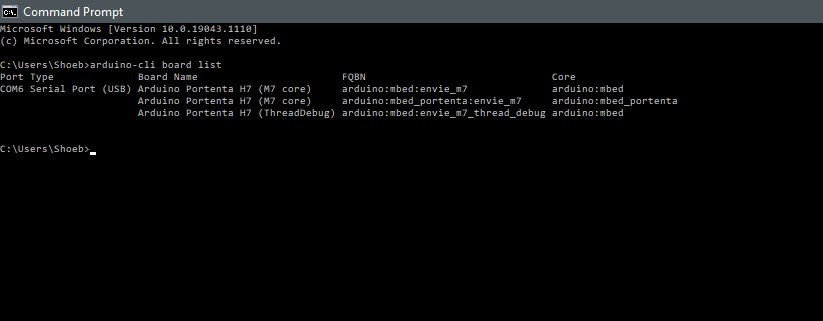
\includegraphics[width=\textwidth]{Arduino/arduino-cli}
        \caption{Installation von Arduino-CLI  }
        \label{ArduinoInstallation}
    \end{figure}


\section{Konfiguration des Arduino CLI}


\URL{https://learn.sparkfun.com/tutorials/efficient-arduino-programming-with-arduino-cli-and-visual-studio-code/introduction-to-the-arduino-cli}

Damit \ac{cli} dir Arduino-Installation finden kann, hilft es, eine Konfigurationsdatei für \ac{cli} zu erstellen. Diese Konfigurationsdatei ist in einem Format YAML\index{YAML} definiert.
Zur Erstellung einer Basis-Konfigurationsdatei kann \ac{cli}  verwendet werden, in dem in einer Kommandozeile 

\medskip

\SHELL{arduino-cli.exe config init}

\medskip

eingegeben wird. Dieser Befehl erstellt eine neue Datei \FILE{.cli-config.yml}. Dort sind alle notwendigen Parameter deklariert. Die Standardeinstellungen der Konfigurationsdatei sind in Abbildung~\ref{KonfigBild} dargestellt. Folgende Parameter müssen in der Regel geändert werden:

\begin{itemize}
    \item \SHELL{sketchbook\_path}: Verzeichnis des Arduino-Sketche. Hier werden alle Bibliotheken und Hardware-Definitionen installiert.
    \item \FILE{arduino\_data}:  Installationsort des Arduino-Boards und des Bibliotheksmanagers. In den meisten Fällen sollte dies nicht geändert werden müssen.
\end{itemize}


Die anderen Optionen können in der Regel auf ihren Standardwerten bleiben.


\begin{figure}
    \begin{center}
        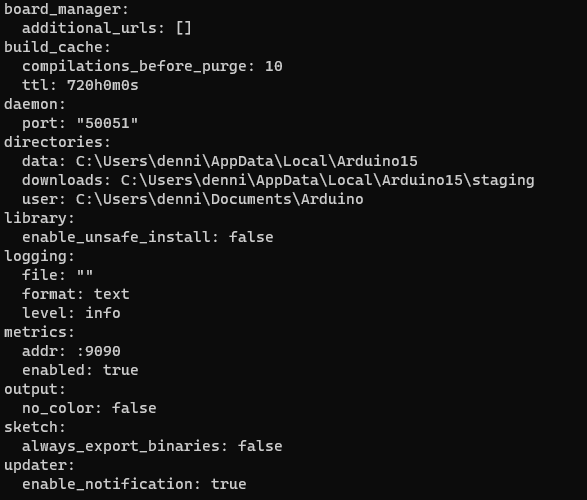
\includegraphics[width=9cm]{Arduino/CLI/StandardConfig.png}
        \caption{Standardeinstellungen der Konfigurationsdatei}
        \label{KonfigBild}
    \end{center}
\end{figure}


\Mynote{Welche Möglichkeiten gibt es in der Konfigurationsdatei?}


\section{Funktionsübersicht}


Die Datei \FILE{README.md} im GitHub-Repository  ``Arduino CLI'' enthält eine hervorragende Übersicht über die Funktionen und Möglichkeiten.\cite{ArduinoCLIGit:2022} 


Folgende Funktionen stehen zur Verfügung \cite{ArduinoCLI:2018}:

\begin{itemize}
  \item \SHELL{arduino-cli}
  \item \SHELL{board}
    \begin{itemize}
      \item \SHELL{board attach}
      \item \SHELL{board details}
      \item \SHELL{board list}
      \item \SHELL{board listall}
      \item \SHELL{board search}
    \end{itemize}
  \item \SHELL{burn-bootloader}
  \item \SHELL{cache}
  \item \SHELL{cache clean}
  \item \SHELL{compile}
  \item \SHELL{completion}
  \item \SHELL{config}
    \begin{itemize}
      \item \SHELL{config dump}
      \item \SHELL{config init}
      \item \SHELL{config add}
      \item \SHELL{config delete}
      \item \SHELL{config remove}
      \item \SHELL{config set}
  \end{itemize}
  \item \SHELL{core}
    \begin{itemize}
      \item \SHELL{core download}
      \item \SHELL{core install}
      \item \SHELL{core list}
      \item \SHELL{core search}
      \item \SHELL{core uninstall}
      \item \SHELL{core update-index}
      \item \SHELL{core upgrade}
    \end{itemize}
  \item \SHELL{daemon}
  \item \SHELL{debug}
  \item \SHELL{lib}
    \begin{itemize}
      \item \SHELL{lib deps}
      \item \SHELL{lib download}
      \item \SHELL{lib examples}
      \item \SHELL{lib install}
      \item \SHELL{lib list}
      \item \SHELL{lib search}
      \item \SHELL{lib uninstall}
      \item \SHELL{lib update-index}
      \item \SHELL{lib upgrade}
    \end{itemize}
  \item \SHELL{monitor}
  \item \SHELL{outdated}
  \item \SHELL{sketch}
    \begin{itemize}
      \item \SHELL{sketch archive}
      \item \SHELL{sketch new}
    \end{itemize}
  \item \SHELL{update}
  \item \SHELL{upgrade}
  \item \SHELL{upload}
  \item \SHELL{version}
\end{itemize}


\subsection{Grundfunktionen}

Als Grundfunktionen werden die Funktionen definiert, die notwendig sind, um einen fertigen Sketch auf einen Arduino zu laden. Die Kommunikation mit einem angeschlossenen Arduino wird später mit Hilfe des seriellen Monitors umgesetzt. 

\bigskip

Die erste Grundfunktion ist der Befehl \SHELL{board list}. Mit diesem lassen sich alle am PC angeschlossenen Arduino Boards mit zusätzlichen Informationen -- wie beispielsweise dem verwendeten Port oder dem Kern des Boards -- anzeigen. Diese Informationen sind für die Verwendung des korrekten Boards  notwendig.


Die Befehle \SHELL{core list} und \SHELL{core install} sind ebenfalls notwendig. Mit dem Befehl \SHELL{core list} können die bereits installierten Kerne aufgelistet werden. Falls der unter \SHELL{board list} angegebene Kern nicht installiert sein sollte, lässt sich dieser mit Befehl \SHELL{core install} hinzufügen. 

Die  dritte Grundfunktion ist  der Befehl \SHELL{lib} mit den Erweiterungen \SHELL{lib list} und \SHELL{lib install}. Mit dem Befehl \SHELL{lib list} lässt sich prüfen, welche Bibliotheken auf dem System bereits installiert sind. Würde für einen Sketch eine zusätzliche Bibliothek benötigt, könnte diese mit dem Befehl \SHELL{lib install} installiert werden.

\Mynote{Ablaufdiagramm zur Verwendung der Befehle}

Mit diesen Grundfunktionen können die Vorbereitungen für das Kompilieren und Hochladen eines Sketches getroffen werden. Mit der Ausführung des Befehls \SHELL{compile} wird ein Sketch in  für ein ausgewähltes Board lesbaren Code übersetzt. Das anschließende Hochladen eines kompilierten Sketches auf ein Board erfolgt mit dem Befehl \SHELL{upload}. Dabei wird der aus dem Befehl \SHELL{board list} bekannte Port des Boards als Ziel für den Upload genannt. Die Grundfunktionen sind in der Tabelle  \ref{CLITabGrundfunktionen} zusammengefasst.

\begin{center}
  \begin{table}[h]
    \captionabove{Liste der Grundfunktionen}
    \begin{tabular}{c|c|l}
      Nr. & Grundfunktion & Beschreibung \\ \hline
      1 & \SHELL{board list} & Auflisten der angeschlossenen Arduinos mit Zusatzinfo \\
      2 & \SHELL{core list}/\SHELL{install} & Auflisten und Installieren von Kernen \\
      3 & \SHELL{lib list}/{install} & Auflisten und Installieren von Bibliotheken \\
      4 & \SHELL{compile} & Kompilieren eines Sketches für ein spezielles Board \\
      5 & \SHELL{upload} & Hochladen eines Sketches auf einen Arduino \\
    \end{tabular}
    \label{CLITabGrundfunktionen}
  \end{table}
\end{center}


\section{Erste Schritte mit dem Arduino Nano 33 BLE Sense Lite mit Hilfe des CLI}

\subsection{Erkennung der angeschlossenen Boards}


Mit Hilfe von \ac{cli} kann abgefragt werden, welche Boards installiert sind:

\medskip


\SHELL{arduino-cli board listall}

\medskip

Falls das angeschlossenes Board vermisst wird, muss es installiert werden:

\medskip

\SHELL{arduino-cli core install arduino:avr}

\medskip

Mit Hilfe von \ac{cli} kann abgefragt werden, welche Boards angeschlossen sind:

\medskip


\SHELL{arduino-cli board list}



So kann nach dem Anschließen des Arduinos an einen PC mit dem Befehl \glqq arduino-cli board list\grqq geprüft werden, ob das Board von dem Computer erkannt wird. Die Funktion \glqq board list\grqq besitzt mehrere Rückgabewerte. So wird der Port, über den das Board mit dem PC verbunden ist, das Protokoll, der Typ, der Platinenname und der FQBN sowie Kern, wie in Abb. \ref{DBboardlist} dargestellt, zurückgegeben.

\begin{figure}[h]
    \begin{center}
        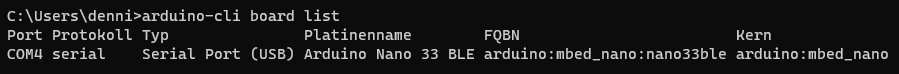
\includegraphics[width=11cm]{Arduino/CLI/boardlist.png}
        \caption{Rückgabewerte der \glqq board list\grqq-Funktion}
        \label{DBboardlist}
    \end{center}
\end{figure}

\begin{figure}[h]
    \begin{center}
        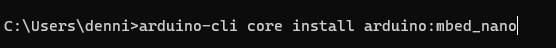
\includegraphics[width=11cm]{Arduino/CLI/KernInstallieren.png}
        \caption{Installieren des Kerns für den Arduino Nano 33 BLE Sense Lite}
        \label{KernInstallieren}
    \end{center}
\end{figure}


Zu Beginn sollte der richtige Kern für den Arduino Nano 33 BLE Sense Lite, wie in Abb. \ref{KernInstallieren} gezeigt, installiert werden. Dies erfolgt mit dem \glqq core install\grqq{}-Befehl und dem richtigen Kernnamen, der aus Abbildung \ref{DBboardlist} entnommen werden kann.


\subsection{Erstellung eines neuen Sketches}

Der erste Schritt ist die Erstellung eines neuen Sketches:

\medskip

\SHELL{arduino-cli sketch new cli\_test}

\medskip

Dieser Befehl erstellt ein Verzeichnis mit dem Namen \FILE{cli\_test}, die eine Datei mit dem gleichen Namen enthält.

\subsection{Kompilieren eines Sketches}

Die Funktion \glqq compile\grqq{} von \ac{cli} kann verwendet werden, um einen Sketch für jedes unterstützte Board zu kompilieren. Die entscheidende Option, die diese Funktion benötigt, ist der Board-Typ, der mit der Option \SHELL{--fqbn} angegeben werden kann. Die Abkürzung \SHELL{fqbn} bedeutet \glqq fully-qualified board name\grqq, was \glqq vollqualifizierter Board-Name\grqq{} bedeutet. Beispielsweise stehen folgende Boards zur Verfügung:


\begin{itemize}
    \item Arduino Uno: \SHELL{arduino:avr:uno}
    \item Arduino Mega: \SHELL{arduino:avr:mega}
    \item SparkFun RedBoard oder SparkFun BlackBoard: \SHELL{SparkFun:avr:RedBoard}; dies erfordert die zusätzliche Installation der Definition \glqq SparkFun avr board\grqq.
    \item  SparkFun SAMD21 Mini: \SHELL{SparkFun:samd:samd21\_mini}; dies erfordert die zusätzliche Installation der Definition \glqq SparkFun samd board\grqq.
    \Mynote{Portenta H7 und Nicla Vision fehlen}
\end{itemize}

Die möglichen Boards sind wie folgt aufgebaut:  \SHELL{manufacturer:architecture:board}.

\bigskip

Mit dem folgenden Kommando kann der Beispiel-Sketch, der sich im Ordner  \PATH{C:/Users/user.name/Documents/Arduino/} befindet, für einen Arduino UNO kompiliert werden.:

\medskip

\SHELL{arduino-cli compile --fqbn arduino:avr:uno C:/Users/user.name/Documents/Arduino/cli\_test}

\medskip

In der Abbildung \ref{ArduinoCompile} sieht man die Meldungen von \ac{cli}.

\begin{figure}
    \centering
    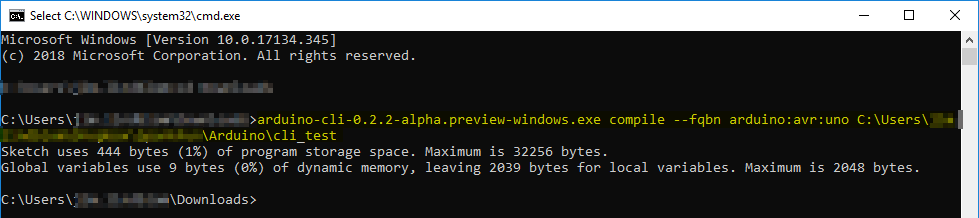
\includegraphics[width=\textwidth]{Arduino/arduino-cli-compile-cmd.png}
    \caption{Kompilieren eines Sketches mit \ac{cli}}
    \label{ArduinoCompile}
\end{figure}


Es können folgende Flags hinzugefügt werden:

\begin{itemize}
    \item Ausführlich \SHELL{-v}:  Nützlich, wenn alle Optionen und Dateien angezeigt werden sollen, die in Ihrem Sketch kompiliert werden.
    \item Build Pfad \SHELL{--build-path [string]}: Nützlich, wenn die kompilierten Objekt- und Hex-Dateien zu speichern sind. Auf meinem Windows-System muss der Wert dieses Parameters ein vollständiger Pfad sein.	
\end{itemize}

\subsection{Hochladen eines Sketches}

Ein kompilerter Sketch kann hochgeladen werden. Wie der Kompilierbefehl erfordert auch der Upload-Befehl eine \SHELL{--fqbn}. Außerdem wird eine serielle Schnittstelle zum Hochladen benötigt, die mit der Option \SHELL{-p} festgelegt wird.
Der folgende Befehl lädt den Beispiel-Sketch an einen Windows-COM-Anschluss auf COM18 hoch:

\medskip

\SHELL{arduino-cli upload -p COM18 --fqbn -v arduino:avr:uno C:/Users/user.name/Documents/Arduino/cli\_test}

\medskip


Falls es ordnungsgemäß durchgeführt wurde, sollte die RX/TX-LEDs des Arduinos zu blinken beginnen und kurz darauf einen leeren Sketch auszuführen.


\subsection{Installation von Bibliotheken}

Falls eine Bibliothek benötigt wird, so kann zunächst mit dem Kommando 

\medskip

\SHELL{arduino-cli lib search ethernet}

\medskip

on die Bibliothek, hier \SHELL{ethernet}, installiert ist. Mit dem Befehl

\medskip

\SHELL{arduino-cli lib install "{}UIPEthernet"}

\medskip

wird sie dann installiert.

\subsection{Beispiel \glqq Hello World\grqq}

Um das Kompilieren eines Sketches sowie das anschließende Hochladen mit Hilfe des Arduino-CLI zu demonstrieren, soll das \glqq Hello World!\grqq{}-Pendant für Mikrocontroller verwendet werden. Dafür wird ein einfacher Sketch, der die LED des Arduinos zum Blinken bringt, benutzt.

\begin{lstlisting}{Name}
    void setup(){
        pinMode(LED_BUILTIN, OUTPUT);
    }
    void loop(){
        digitalWrite(LED_BUILTIN, HIGH);
        delay(1000);
        digitalWrite(LED_BUILTIN, LOW);
        delay(1000);
    }
\end{lstlisting}

In der zu Beginn einmalig ausgeführten \SHELL{setup()}-Funktion wird die eingebaute \acs{led} als Output definiert \SHELL{pinMode(LED\_BUILTIN, OUTPUT)}. Dadurch lässt sich die LED später ansteuern. Innerhalb der \SHELL{loop()}-Funktion wird die LED zunächst eingeschaltet \SHELL{digitalWrite(LED\_BUILTIN, HIGH)} und mit einer Verzögerung von einer Sekunde \SHELL{delay(1000)} wieder abgeschaltet \SHELL{digitalWrite(LED\_BUILTIN}, \SHELL{LOW)}. Vor dem erneuten Einschalten der LED zu Beginn der Schleife wird am Schleifenende nochmal eine Sekunde gewartet um den blinkenden Effekt zu erzielen.

Um den Sketch zu kompilieren, kann der zuvor als Grundfunktion definierte Befehl \SHELL{compile}, wie in Abb. \ref{Kompilieren} dargestellt, verwendet werden.

\begin{figure}[h]
    \begin{center}
        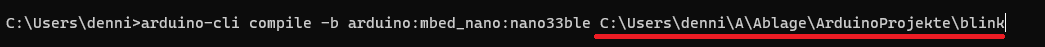
\includegraphics[width=11cm]{Arduino/CLI/Kompilieren.png}
        \caption{Für das Kompilieren des Blink-Sketches wird der Dateipfad zu dem Sketch mit angegeben (rot unterstrichen). Außerdem sollte der FQBN des Arduinos, für den der Sketch kompiliert wird, genannt werden.}
        \label{Kompilieren}
    \end{center}
\end{figure}

Anschließend kann der kompilierte Sketch mit Hilfe der \glqq upload\grqq{}-Funktion auf den Arduino hochgeladen werden. Dafür wird, wie in Abb. \ref{Hochladen} dargestellt, der Speicherpfad zu dem Sketch angegeben. Dadurch erfolgt das Hochladen der kompilierten Daten für den angegebenen Sketch.

\begin{figure}[h]
    \begin{center}
        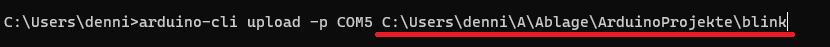
\includegraphics[width=11cm]{Arduino/CLI/Hochladen.png}
        \caption{Hochladen des kompilierten Sketches aus dem Temp-Ordner}
        \label{Hochladen}
    \end{center}
\end{figure}


Nach dem erfolgreichen Upload beginnt die in Abb. \ref{LEDtest} gezeigte LED des Arduino Nano 33 BLE Sense Lite zu blinken.

\begin{figure}[h]
    \begin{center}
        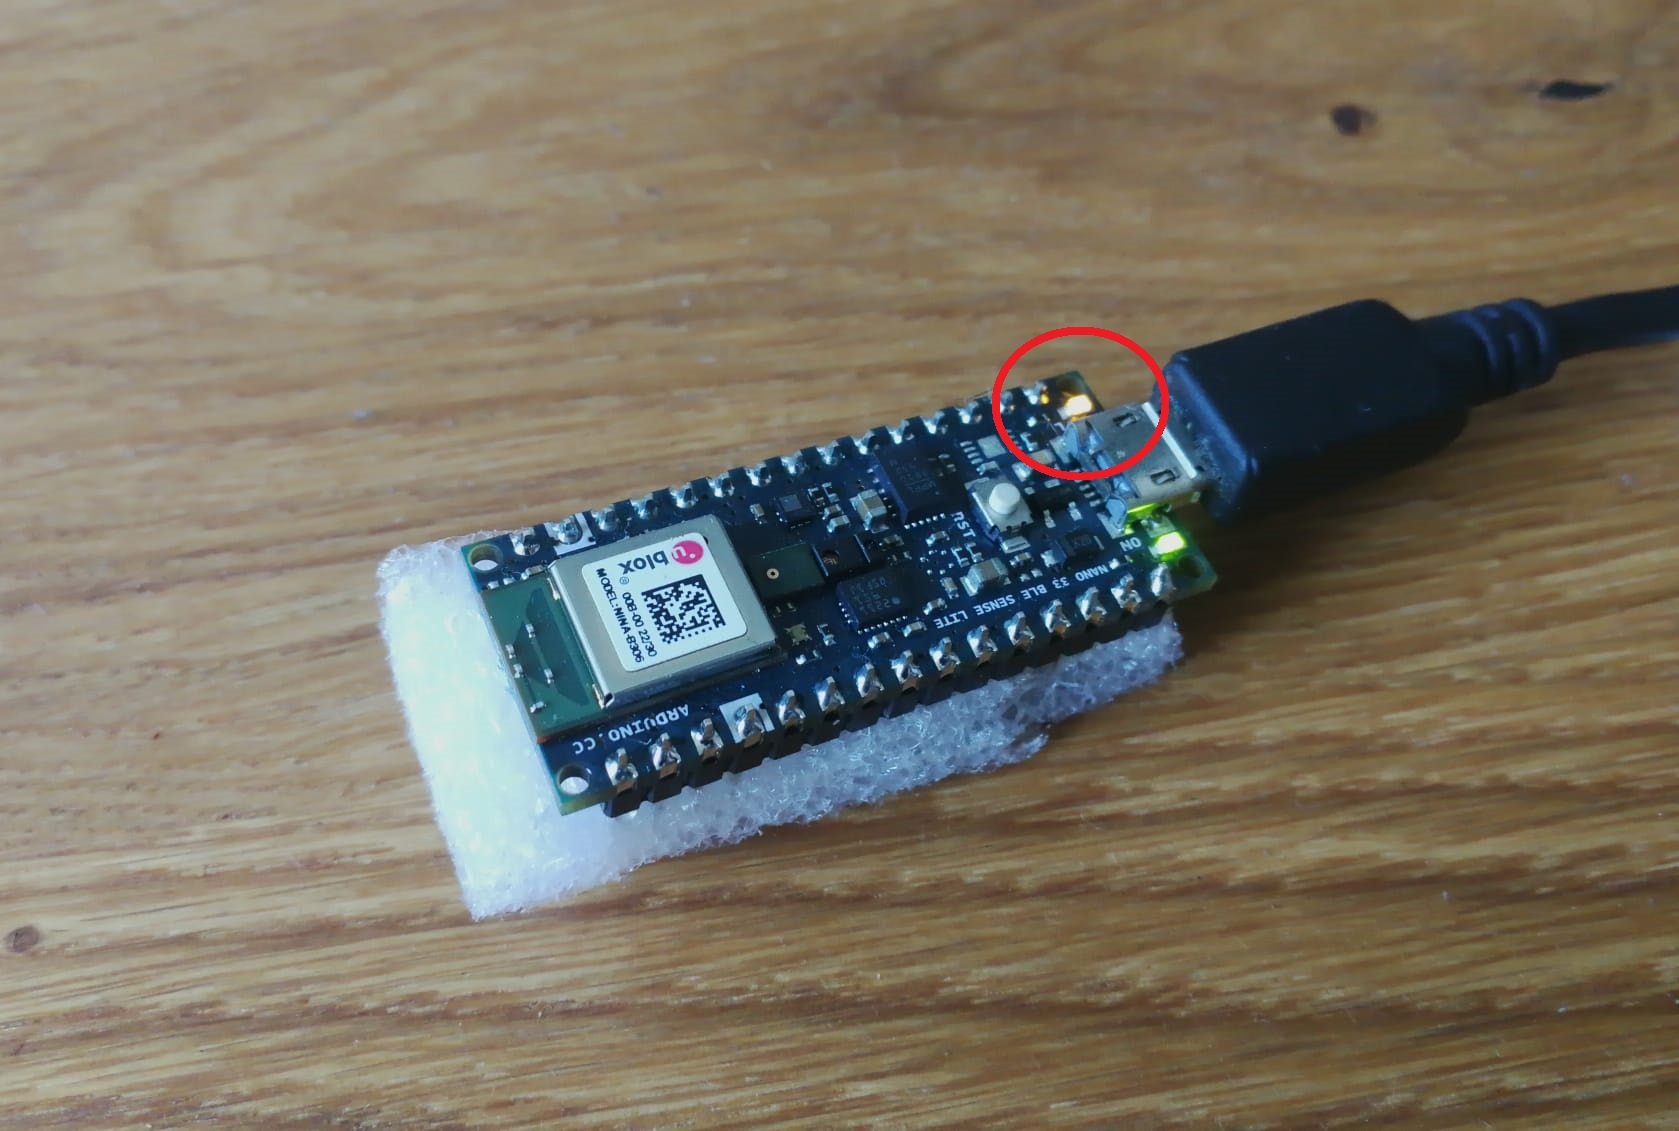
\includegraphics[width=11cm]{Arduino/CLI/LEDtesten.jpeg}
        \caption{Die orange LED des Arduinos beginnt zu blinken}
        \label{LEDtest}
    \end{center}
\end{figure}


\section{Beschreibung der Software auf dem PC}

Um einen erhöhten Automatisierungsgrad zu erreichen und die Potentiale des Arduino-CLI zu demonstrieren, wird ein Batch-Skript zum Testen der Sensoren verwendet. Dabei werden die Ergebnisse in einer Log-Datei dokumentiert. In diesem Abschnitt soll die Funktionsweise des Batch-Skriptes beschrieben werden.

{\small 
\begin{lstlisting}{Name}
@echo off
echo Logdatei Arduino-Setup, %time% Uhr, %date% > setup-log.txt
echo. >> setup-log.txt
echo. >> setup-log.txt
\end{lstlisting}
}

Mit dem Befehl \SHELL{\@echo off} wird die Ausgabe des Skript-Inhaltes bei Ausführung verhindert. Dadurch wird eine ansprechendere Frontend-Programmierung ermöglicht. In der zweiten Zeile wird die Log-Datei erstellt. Beim Erstellen wird mit der Überschrift \SHELL{Logdatei Arduino-Setup} sowie dem Auslesen der Systemzeit \SHELL{\%time\%} und des Datums \SHELL{\%date\%} die erste Zeile des Protokolls versehen. Für die spätere Übersichtlichkeit der Log-Datei folgen zwei leere Zeilen \SHELL{echo. >> setup-log.txt}. Mit dem einmaligen Anwenden des größer als Operators \SHELL{> setup-log.txt} wird eine neue Datei erstellt oder eine Bestehende mit dem gleichen Namen überschrieben. Bei doppelter Anwendung des größer als Operators \SHELL{>> setup-log.txt} wird der linksseitige Inhalt in einer neuen Zeile an eine bestehende Datei angehängt. So wird die Log-Datei Zeile für Zeile beschrieben und nicht einmalig komplett am Ende des Batch-Skriptes.

\begin{lstlisting}{Name}
:: Gegebenenfalls wird der Kern installiert
echo Kernstatus: >> setup-log.txt
arduino-cli core install arduino:mbed_nano >> setup-log.txt
\end{lstlisting}

Kommentare in dem Batch-Skript werden durch zwei aufeinanderfolgende Doppelpunkte gekennzeichnet \SHELL{:: Gegebenenfalls wird der Kern installiert} und sollen die Nachvollziehbarkeit innerhalb des Skriptes erhöhen. Mit dem Befehl \SHELL{echo Kernstatus: >> setup-log.txt} wird in der Log-Datei gekennzeichnet, dass in der nächsten Zeile Informationen über den zu installierenden Kern für den Arduino Nano 33 BLE Sense Lite folgen. Das Arduino-CLI bringt bereits die Intelligenz mit zu prüfen, ob der angegebene Kern schon installiert ist. Sollte dies der Fall sein, erfolgt die entsprechende Dokumentation in der Log-Datei. Das Installieren des Kerns wird mit der Zeile \SHELL{arduino-cli core install arduino:mbed\_nano >> setup-log.txt} initialisiert. Dabei ist der für den Arduino Nano 33 BLE Sense Lite notwendige Kern mit dem Namen \SHELL{arduino:mbed\_nano} angegeben. Der Rückgabewert der Funktion zum Kerninstallation wird in der Log-Datei gespeichert.

\begin{lstlisting}{Name}
echo Es wird nach angeschlossenen Boards gesucht...
:: Auflisten der angeschlossenen Arduinos
echo Folgende Boards sind am PC angeschlossen: >> setup-log.txt
echo.
echo. >> setup-log.txt
arduino-cli board list >> setup-log.txt
arduino-cli board list
echo.
\end{lstlisting}

Zu Beginn dieses Skript-Abschnittes wird zunächst der Nutzer der Software über die Suche nach den angeschlossenen Arduino Platinen informiert \SHELL{echo Es wird nach angeschlossenen Boards gesucht...}. Folgend wird mit dem Befehl \SHELL{echo Folgende Boards sind am PC angeschlossen: >> setup-log.txt} über den Inhalt der nächsten Zeile in der Log-Datei informiert. Die Information darüber welche Arduinos an dem PC angeschlossen sind, kann mit dem Befehl \SHELL{arduino-cli board list}, der hier doppelt ausgeführt wird, gewonnen werden. Bei der ersten Ausführung wird die Rückgabe des Arduino-CLI in der Log-Datei gespeichert \SHELL{>> setup-log.txt}, die zweite Ausführung dient zur Anzeige in dem aktuell ausgeführten Skript. Die Information über die angeschlossenen Arduinos benötigt der Nutzer im nächsten Schritt für eine Eingabe.

\begin{lstlisting}{Name}
:: Abfragen des Portnamens fuer spaeteren Upload 
:: der Sensorentestdatei
set /p port="Bitte den Portnamen des Sense-Lite eingeben und bestaetigen: "
echo Der Port %port% wurde gewaehlt. >> setup-log.txt
\end{lstlisting}

In der Zeile \SHELL{set /p port="Bitte den Portnamen des Sense-Lite eingeben und bestaetigen: "} erfolgt eine Nutzerabfrage. Der Befehl \SHELL{set} ermöglicht das Setzen der Variable \SHELL{port} auf einen bestimmten Wert. Mit dem Zusatz \SHELL{/p} wird dieser bestimmte Wert auf die folgende Nutzereingabe gesetzt. Die Ausführung des Skriptes wird bis zur erfolgreichen Eingabe des Nutzers gestoppt. Die Nutzereingabe beinhaltet den Port des angeschlossenen Arduino Nano 33 BLE Sense Lite. Für die spätere Nachvollziehbarkeit wird der gewählte Port in der Log-Datei mit der Zeile \SHELL{echo Der Port \%port\% wurde gewaehlt. >> setup-log.txt} dokumentiert. 

\begin{lstlisting}{Name}
:: Anlegen des Ordners fuer den kompilierten Sensorentest
set ordner=SensorentestCompiledData
mkdir %ordner%
\end{lstlisting}

Die Variable \SHELL{ordner} bekommt den Wert \SHELL{SensorentestCompiledData} zugewiesen. In der nächsten Zeile \SHELL{mkdir \%ordner\%} wird der Ordner mit dem Namen \PYTHON{SensorentestCompiledData} für das spätere Speichern des kompilierten Sketches angelegt.

\begin{lstlisting}{Name}
:: Gegebenenfalls werden die noetigen Bibliotheken fuer 
:: den Sensorentest installiert
:: Bib fuer IMU
echo Bib fuer IMU >> setup-log.txt
arduino-cli lib install Arduino_LSM9DS1 >> setup-log.txt
echo. >> setup-log.txt
    
:: Bib fuer Farbsensor
echo Bib fuer Farbsensor >> setup-log.txt
arduino-cli lib install Arduino_APDS9960 >> setup-log.txt
echo. >> setup-log.txt
    
:: Bib fuer Druck- und Temperatursensor
echo Bib fuer Druck- und Temperatursensor >> setup-log.txt
arduino-cli lib install Arduino_LPS22HB >> setup-log.txt
echo. >> setup-log.txt
\end{lstlisting}

In der Log-Datei wird jeweils dokumentiert um welche Bibliothek es sich in der folgenden Zeile handelt \SHELL{SensorentestCompiledData}. Anschließend erfolgt mit dem Befehl \SHELL{arduino-cli lib install Arduino\_LSM9DS1 >> setup-log.txt} das Installieren der Bibliothek sowie das Speichern des Rückgabewertes der Installation in der Log-Datei. Eine bereits installierte Bibliothek wird von dem Arduino-CLI erkannt und es folgt eine entsprechende Rückgabe in die Log-Datei. Das Vorgehen ist für alle drei zu installierenden Bibliotheken identisch.

\begin{lstlisting}{Name}
:: Kompilieren des Sensorentest-Sketches
echo Kompilieren des Sensorentest-Sketches: >> setup-log.txt
echo. >> setup-log.txt
arduino-cli compile -b arduino:mbed_nano:nano33ble %cd%\SensortestLite 
--build-path %cd%\%ordner% >> setup-log.txt
\end{lstlisting}

Nachdem die notwendigen Bibliotheken installiert sind, kann der zuvor erstellte Sketch zum Testen der Sensoren kompiliert werden. Das Kompilieren des Sketches für den Arduino Nano 33 BLE Sense Lite erfolgt mit dem Befehl \SHELL{arduino-cli compile -b arduino:mbed\_nano:nano33ble \%cd\%/SensortestLite}. Der hintere Teil des Befehls gibt den Speicherpfad des zu kompilierenden Sketches an. Weiterhin lässt sich der Zielordner für den kompilierten Sketch mit dem Zusatz \SHELL{--build-path \%cd\%/\%ordner\% >> setup-log.txt} definieren. Der Rückgabewert des Kompilierens mit dem Arduino-CLI wird in der Log-Datei gespeichert.

\begin{lstlisting}{Name}
:: Hochladen des kompilierten Sketches auf den Arduino
echo Hochladen des kompilierten Sketches auf den Arduino >> setup-log.txt
arduino-cli upload -p %port% --input-dir %cd%\%ordner% >> setup-log.txt
\end{lstlisting}

Der kompilierte Sketch wird in der Zeile \SHELL{arduino-cli upload -p \%port\% --input-dir}  \SHELL{\%cd\%/\%ordner\% >> setup-log.txt} auf den durch \SHELL{port} angeschlossenen Arduino Nano 33 BLE Sense Lite hochgeladen. Der Speicherpfad der kompilierten Daten wird mit dem Zusatz \SHELL{--input-dir \%cd\%/\%ordner\%} angegeben.

\begin{lstlisting}{Name}
:: Oeffnen des seriellen Monitors
start monitor_log
:: Automatisches Schlieszen des seriellen Monitors nach 4 Sekunden 
:: (n-1 Sekunden, mit n=5)
ping 127.0.0.1 -n 5 > nul
taskkill /im serial-monitor.exe /F
\end{lstlisting}

Mit dem Befehl \SHELL{start monitor\_log} wird ein weiteres Batch-Skript zum Auslesen des seriellen Monitors aufgerufen. Die Zeile \SHELL{ping 127.0.0.1 -n 5 > nul} stoppt die Ausführung der Software für vier Sekunden. Dabei werden fünf Anfragen an den lokalen Rechner gesendet und jeweils eine Sekunde zwischen zwei Anfragen gewartet. Mit \SHELL{> nul} wird die Ausgabe der Antworten ins Leere geleitet und nicht angezeigt. Ist die Zeitspanne von vier Sekunden abgelaufen wird der serielle Monitor zum Auslesen der Sensordaten automatisch mit dem Befehl \SHELL{taskkill /im serial-monitor.exe /F} geschlossen. Über den Zusatz \SHELL{/im} kann das zu schließende Fenster \SHELL{serial-monitor.exe} benannt werden. Das erzwungene Schließen des seriellen Monitors erfolgt mit dem Anhang \SHELL{/F}. Nachdem der serielle Monitor ausgelesen und geschlossen wurde, kann die Software beendet werden. Die Ergebnisse des Sensoren-Tests lassen sich im Anschluss der Log-Datei entnehmen.

Das Öffnen des seriellen Monitors erfolgt in dem Skript \FILE{monitor\_log.bat}.

\begin{lstlisting}{Name}
echo Sensordaten: >> setup-log.txt
echo. >> setup-log.txt
    
echo Der serielle Monitor wird geoeffnet, die Sensordaten werden ausgelesen und in der Logdatei gespeichert...
    
arduino-cli monitor -p %port% >> setup-log.txt
\end{lstlisting}	

Der serielle Monitor kann mittels des Arduino-CLI Befehls \SHELL{arduino-cli monitor} \SHELL{-p \%port\% >> setup-log.txt} geöffnet werden. Dabei wird mit \SHELL{-p \%port\%} die Verbindung für den angegebenen Port hergestellt. Mit dem Zusatz \SHELL{>> setup-log.txt} werden die empfangenen Daten in die Log-Datei geschrieben.

    % Zurzeit nur für Portenta H7
    %  \InputLanguage{../contents/General/}{CommandLineInterface}
    
    \InputLanguage{../contents/General/}{OpenMV}
    
    \InputLanguage{../contents/General/}{OpenMVBlob}
    
    \InputLanguage{../contents/General/}{EdgeImpulse}
    
    \InputLanguage{../contents/General/}{GoogleColab}
    
    \InputLanguage{../contents/General/}{GoogleColabExample}
}



\part{\TRANS{Portenta H7}{Portenta H7}}
	
%%%%%%%%%%%%%%%
%
% $Autor: Wings $
% $Datum: 2020-01-29 07:55:27Z $
% $Pfad: komponenten/Bilderkennung/Produktspezifikation/IntelNCS2/Inhalt/Einleitung.tex $
% $Version: 1785 $
%
%
%%%%%%%%%%%%%%%

\chapter{Einleitung}

{\tiny Quelle: \url{https://www.arduino.cc/pro/tutorials/portenta-h7}}





%%%%%%%%%%%%%%%
%
% $Autor: Wings $
% $Datum: 2020-01-29 07:55:27Z $
% $Pfad: komponenten/Bilderkennung/Produktspezifikation/IntelNCS2/Inhalt/Einleitung.tex $
% $Version: 1785 $
% !TeX spellcheck = en_GB
%
%
%%%%%%%%%%%%%%%

\chapter{Introduction}

{\tiny Quelle: \url{https://www.arduino.cc/pro/tutorials/portenta-h7}}




Arduino Portenta H7 board is a dual core unit which has STM32H7 ARM Cortex®-M7 running at 480Mhz and Cortex®-M4 running at 240Mhz. This means it is capable of reading and executing two instructions at the same time. These two processors run the Mbed OS , which is an embedded real time operating system(RTOS) that is optimized for low-power microcontrollers. The interesting part of this dual core processor is that both the processors can communicate with each other and other peripherals on the board.  This is done by a mechanism called Remote procedure Call(RPC) which helps in calling functions on the other processor. The two processors can run Arduino sketches on top of the Mbed OS,  MicroPython/JavaScript via an interpreter, native Mbed applications and TensorFlow Lite.

The Arduino core sits on top of the Mbed OS and acts as a middleware which allows programs to leverage the Mbed OS APIs for storage, communication, security, and other hardware interfaces.

The portenta H7 also has an on-chip GPU Chrom-ART Accelerator, which makes it able to connect an external monitor to build a dedicated embedded computer. In addition, it also has a wireless module which is able to connect WiFi and Bluetooth simultaneously. The WiFi interface can also be utilized as an access point thereby creating its own WiFi network and allowing other devices to connect to it.
Another interesting feature of portenta H7 is it has two 80-pin high density connectors at the bottom of the board in order to connect to other devices.  It also has a USB type-C port  which is used to power the board, connect to a display and can also be utilized as a USB hub. 
Some of the Industrial applications of the Arduino Portenta h7 include\cite{PortentaH7:2021}

\begin{itemize}
	
	\item High-end industrial machinery
	\item	Laboratory equipment
	\item	Computer vision
	\item	PLCs
	\item	Industry-ready user interfaces
	\item	Robotics controller
	\item	Mission-critical devices
	\item	Dedicated stationary computer
	\item	High-speed booting computation 
\end{itemize}



\chapter{Hardware}

%%%%%%%%%%%%%%%%%%%%%%%%
%
% $Autor: Wings $
% $Datum: 2020-07-24 09:05:07Z $
% $Pfad: GDV/Vortraege/latex - Ausarbeitung/Kapitel/Einleitung.tex $
% $Version: 4732 $
%
%%%%%%%%%%%%%%%%%%%%%%%%

\chapter{PortentaH7}
	The PortentaH7 is a high-performance microcontroller board developed by Arduino. It is designed to cater to professional applications, offering robust computing power, advanced features, and versatility. Here are some key aspects of the PortentaH7:
	
	Within the H7 family, there are two variants; H7 Lite and H7 Lite Connected. All the three boards and their differences are presented in this datasheet.
	
	\textbf{Target Areas}: 
	Laboratory equipment, Computer vision
	
	\begin{figure}
		\begin{center}
			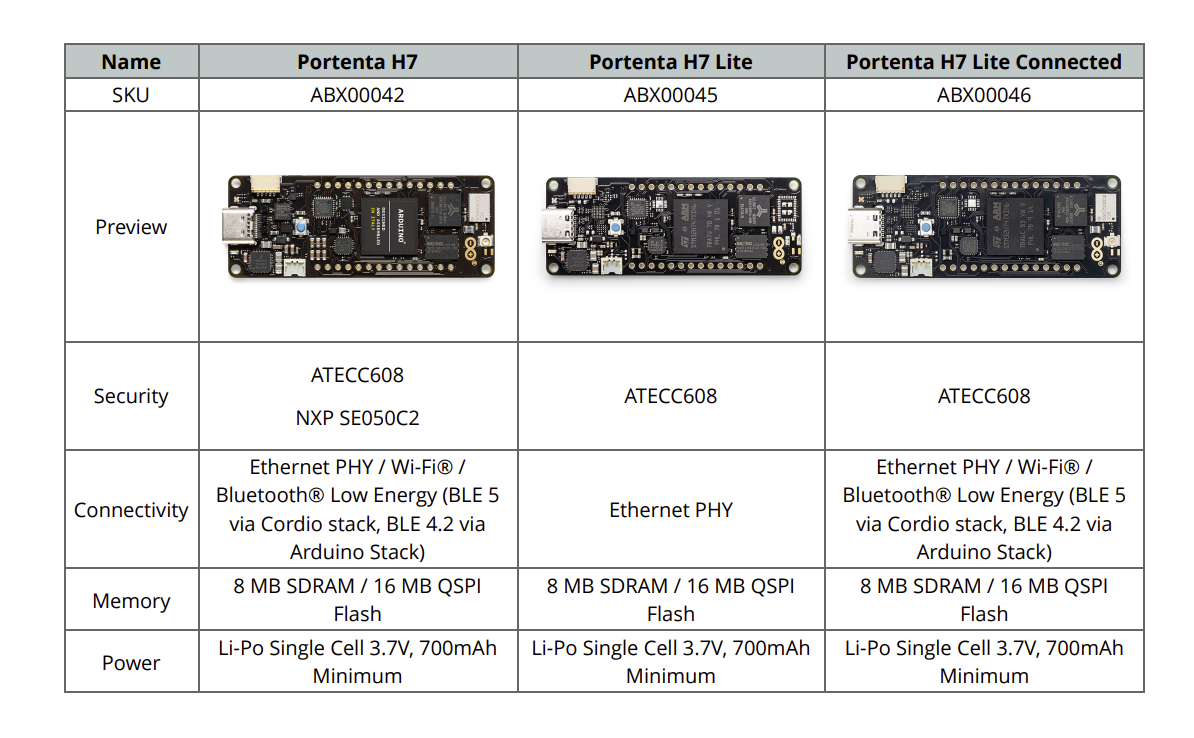
\includegraphics[width=0.7\linewidth]{Images/PortentaH7/TypesofPortentaH7.png}
			\caption{Types of PortentaH7}
			\label{Types}
		\end{center}
	\end{figure}
	
\section{Key Features:}

\textbf{Dual-core Processor:}

\begin{itemize}
	\item Cortex-M7: Runs at up to 480 MHz.
	\item Cortex-M4: Runs at up to 240 MHz.
	\item These cores can operate simultaneously, allowing for efficient parallel processing and real-time application execution.
\end{itemize}

\textbf{Memory:}
\begin{itemize}
	\item RAM: 1 MB of SRAM and 16 MB of SDRAM.
	\item Flash Storage: 8 MB.
\end{itemize}

\textbf{Connectivity:}
\begin{itemize}
	\item $<$ Built-in GPU for handling advanced graphical interfaces. 
	\item $<$ Supports an external display through a dedicated connector.
\end{itemize}

\textbf{Security:}
\begin{itemize}
	\item Hardware cryptography support for secure applications.
	\item Secure boot and secure firmware updates.
\end{itemize}

\textbf{Expansion Options:}
\begin{itemize}
	\item Compatible with Arduino MKR and \textbf{Portenta Vision Shield.}
	\item High-density connectors for custom hardware extensions.
\end{itemize}

\textbf{Operating Systems:}
\begin{itemize}
	\item Capable of running high-level OS like Arm Mbed OS or real-time operating systems (RTOS).
	\item Compatible with Arduino programming environment and libraries.
\end{itemize}

\textbf{Power Management:}
\begin{itemize}
	\item Multiple power supply options: USB-C, Li-Po battery, or external sources.
	\item Low power modes for energy-efficient applications.
\end{itemize}

\textbf{Applications:} \newline
	The Portenta H7 is suitable for a wide range of professional applications, including but not limited to:
\begin{itemize}
	\item \textbf{Industrial IoT:} Real-time monitoring, data acquisition, and control systems.
	\item \textbf{Edge Computing:} Local data processing and decision-making.
	\item \textbf{AI and Machine Learning:} On-device inference and analytics.
	\item \textbf{Robotics:} Advanced motor control and sensor integration.
	\item \textbf{Smart Devices:} Connected appliances, home automation, and wearables.
\end{itemize}

\section{Onboard Sensors with Examples}

	\subsection{Murata 1DX Bluetooth® 5.1}
		The onboard Bluetooth® module of the Portenta H7 offers low energy Bluetooth® functionality, in order to provide the board with the flexibility to be easily connected to devices which also support Bluetooth® Low Energy, such as the Arduino Nano 33 IoT or most modern smartphones. Compared to classic Bluetooth®, Low Energy Bluetooth® is intended to provide considerably reduced power consumption and cost while maintaining a similar communication range. \cite{bluetoothPortentaH7:2024}
		
		\subsubsection{Overview}
			In this Example we will enable low energy Bluetooth® on the Portenta H7 to allow an external Bluetooth® device to control the built-in LED either by turning it on or off.
	
		\subsubsection{Goals}
			\begin{itemize}
				\item Enabling Bluetooth® Low Energy connectivity on the Portenta H7.
				\item Connecting the Portenta to an external Bluetooth® Low Energy Mobile Application (In this case nRF Connect by Nordic Semiconductor).
			\end{itemize}
			
		\subsubsection{Required Hardware and Software}
			\begin{itemize}
				\item Portenta H7 (ABX00042) or Portenta H7 Lite Connected (ABX00046)
				\item USB-C® cable (either USB-A to USB-C® or USB-C® to USB-C®)
				\item Arduino IDE 1.8.13+ or Arduino Pro IDE 0.0.4+
				\item Mobile device, phone or tablet
				\item nRFconnect or equivalent tool downloaded on your mobile device: nRF Connect for iOS or nRF Connect for android
			\end{itemize}
			
		\subsubsection{Instructions}
			\begin{itemize}
				\item \textbf{Configuring the Development Environment:} To communicate with the Portenta H7 via Bluetooth®, you need to upload a pre-built sketch that starts a Bluetooth® network and allows your mobile device, which will be used to control the LEDs, to connect to it. The sketch uses the ArduinoBLE Library that enables the Bluetooth® Low Energy module and handles important functions, such as scanning, connecting and interacting with services provided by other devices. You will also be using a third party application (e.g. nRF Connect), running on your mobile device in order to connect your device to the board and help you control the built-in LED. ~\ref{Bluetooth-portentaH7}
					\begin{figure}
						\begin{center}
							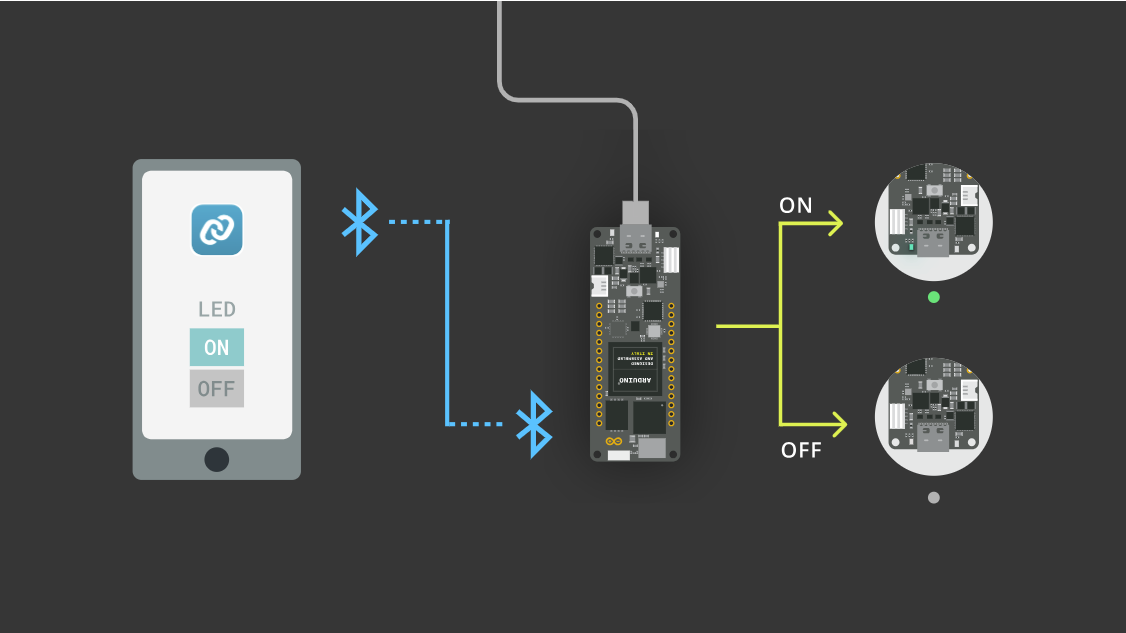
\includegraphics[width=0.7\linewidth]{Images/PortentaH7/Bluetooth-portentaH7.png}
							\caption{Bluetooth-portentaH7}
							\label{Bluetooth-portentaH7}
						\end{center}
					\end{figure}
					
				\item \textbf{1. The Basic Setup:} Begin by plugging in your Portenta board to the computer using a USB-C® cable and open the Arduino IDE. If this is your first time running Arduino sketch files on the board, we suggest you check out how to set up the Portenta H7 for Arduino before you proceed.
					\begin{figure}
						\begin{center}
							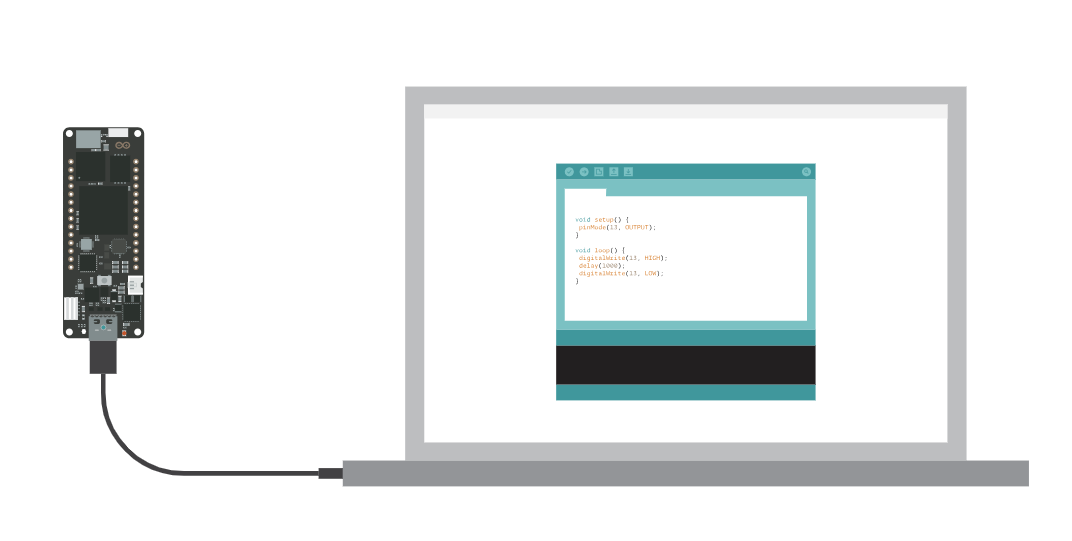
\includegraphics[width=0.7\linewidth]{Images/PortentaH7/PortentaH7-connection.png}
							\caption{PortentaH7-connection}
							\label{PortentaH7-connection}
						\end{center}
					\end{figure}
				
				\item \textbf{2. Install the ArduinoBLE Library:} You will need to install the ArduinoBLE library in the Arduino IDE you are using. To install the library go to : Tools > Manage Libraries... type ArduinoBLE and click Install. Make sure you install ArduinoBLE version 1.1.3 or higher. ~\ref{Bluetooth-Library}
					\begin{figure}
						\begin{center}
							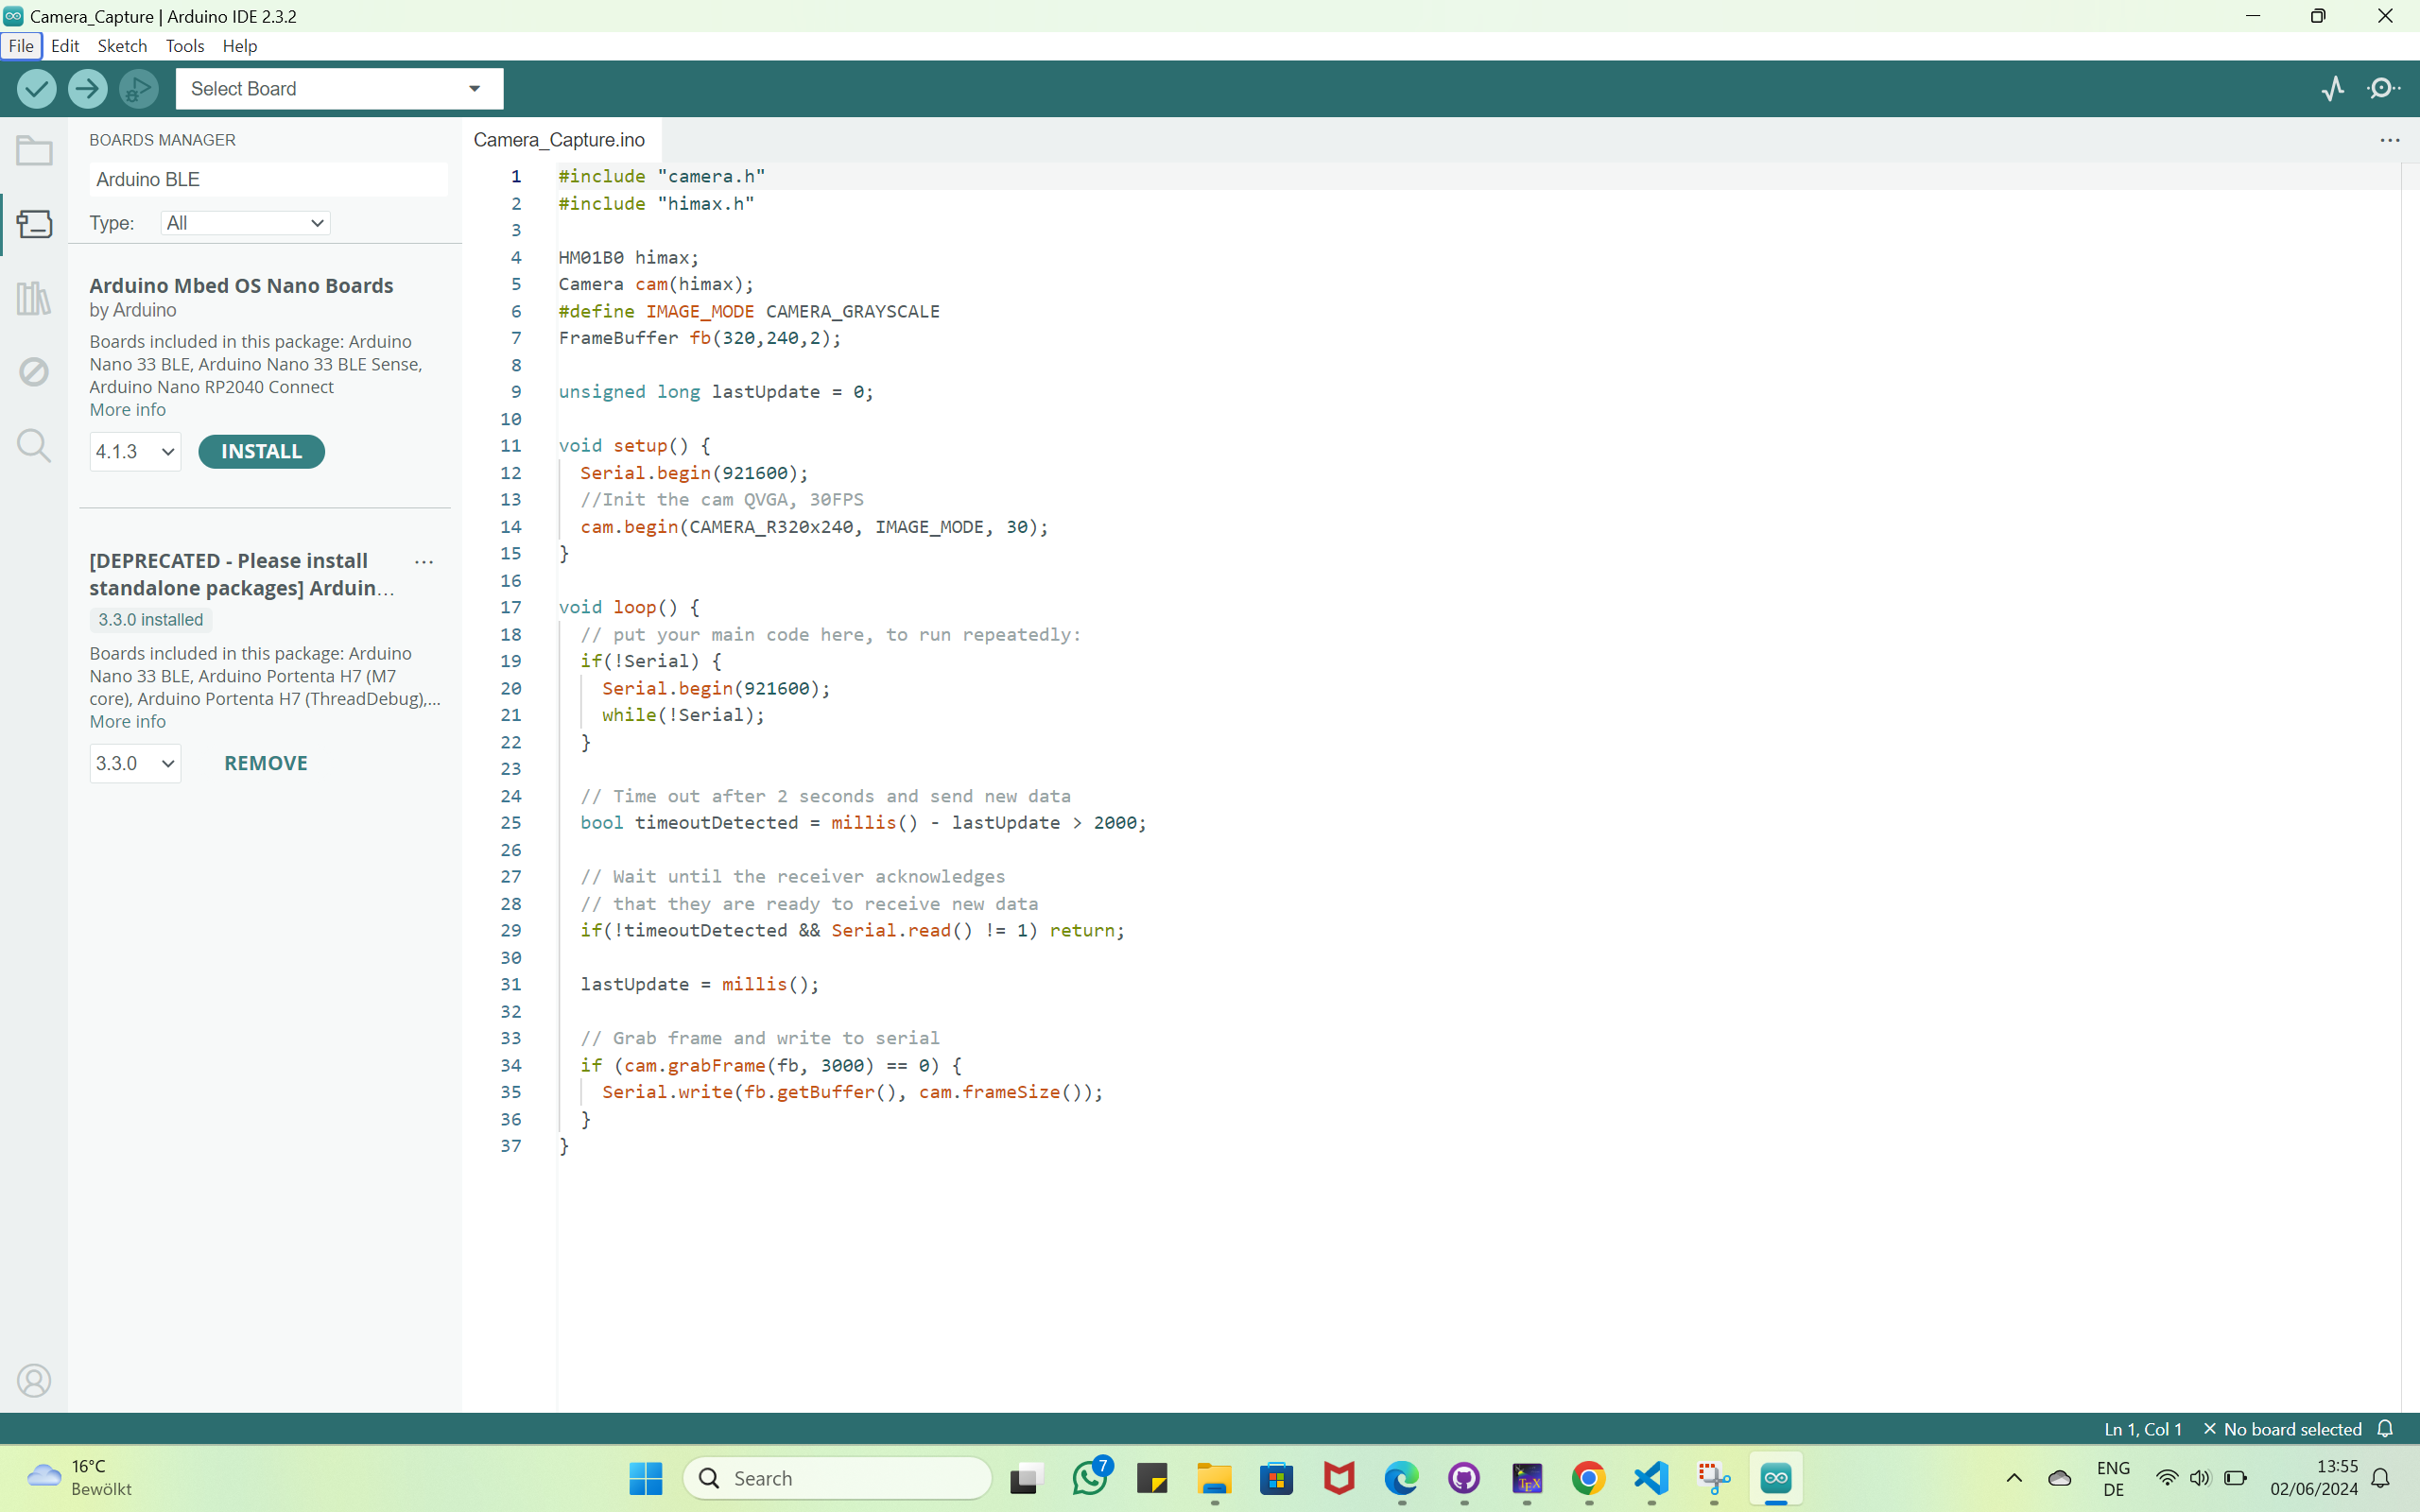
\includegraphics[width=0.7\linewidth]{Images/PortentaH7/Bluetooth-Library.png}
							\caption{Bluetooth-Library}
							\label{Bluetooth-Library}
						\end{center}
					\end{figure}
				
				\item \textbf{3. Create the Bluetooth® Low Energy Sketch:} Let's program the Portenta with the following example sketch. If the Bluetooth® Low Energy module has been initialized correctly, you will see the blue LED lighting up for one second after uploading the sketch. If it fails, you will see the red LED lighting up instead. Copy and paste the following code into a new sketch in your IDE or download it from Arduino-Pro-Tutorials in the Arduino IDE and open it from: Examples > Arduino-Pro-Tutorials > BLE Connectivity on Portenta H7 > PortentaBLE 
					\begin{lstlisting}
						#include <ArduinoBLE.h>
						
						BLEService ledService("19b10000-e8f2-537e-4f6c-d104768a1214");
						
						// Bluetooth Low Energy LED Switch Characteristic - custom 128-bit UUID, read and writable by central
						BLEByteCharacteristic switchCharacteristic("19b10000-e8f2-537e-4f6c-d104768a1214", BLERead | BLEWrite);
						
						const int ledPin = LED-BUILTIN; // Pin to use for the LED
						
						void setup() {
							Serial.begin(9600);
							//while (!Serial);   // Uncomment to wait for serial port to connect.
							
							// Set LED pin to output mode
							pinMode(ledPin, OUTPUT);
							digitalWrite(ledPin, HIGH);
							
							// Begin initialization
							if (!BLE.begin()) {
								Serial.println("Starting Bluetooth Low Energy failed!");
								digitalWrite(LEDR, LOW);
								delay(1000);
								digitalWrite(LEDR, HIGH);
								
								// Stop if Bluetooth Low Energy couldn't be initialized.
								while (1);
							}
							
							// Set advertised local name and service UUID:
							BLE.setLocalName("LED-Portenta-01");
							BLE.setAdvertisedService(ledService);
							
							// Add the characteristic to the service
							ledService.addCharacteristic(switchCharacteristic);
							
							// Add service
							BLE.addService(ledService);
							
							// Set the initial value for the characeristic:
							switchCharacteristic.writeValue(0);
							
							// start advertising
							BLE.advertise();
							digitalWrite(LEDB, LOW);
							delay(1000);
							digitalWrite(LEDB, HIGH);
							Serial.println("BLE LED Control ready");
						}
						
						void loop() {
							// Listen for Bluetooth Low Energy peripherals to connect:
							BLEDevice central = BLE.central();
							
							// If a central is connected to peripheral:
							if (central) {
								Serial.print("Connected to central: ");
								// Print the central's MAC address:
								Serial.println(central.address());
								digitalWrite(LEDB, HIGH);
								delay(100);
								digitalWrite(LEDB, LOW);
								delay(100);
								digitalWrite(LEDB, HIGH);
								
								// While the central is still connected to peripheral:
								while (central.connected()) {
									// If the remote device wrote to the characteristic,
									// Use the value to control the LED:
									if (switchCharacteristic.written()) {
										if (switchCharacteristic.value()) {   // Any value other than 0
											Serial.println("LED on");
											digitalWrite(ledPin, LOW);          // Will turn the Portenta LED on
										} else {                             
											Serial.println("LED off");
											digitalWrite(ledPin, HIGH);         // Will turn the Portenta LED off          
										}
									}
								}
								
								// When the central disconnects, print it out:
								Serial.print("Disconnected from central: ");
								Serial.println(central.address());    
								digitalWrite(LEDB, HIGH);
								delay(100);
								digitalWrite(LEDB, LOW);
								delay(100);
								digitalWrite(LEDB, HIGH);
							}
						}    
								
					\end{lstlisting}
					
					In this example, you use a pre-defined Bluetooth number code pre-setup for controlling a device's LED. This code can also be referred to as GATT codes, which define how two Bluetooth® low energy devices transfer data. Once a connection is established with a device, its respective GATT code, which is a 16 bit identifier, is stored in a lookup table for future reference.
					
					These GATT codes are very long, but, in this example, it is always the same code:
					\begin{lstlisting}
						BLEService ledService("19b10000-e8f2-537e-4f6c-d104768a1214"); // BLE LED Service
					\end{lstlisting}	
					
				\item \textbf{4. Upload the Sketch:} Double press the reset button so the built-in LED is slowly pulsing green. Then, select your board in the menu: Tools > Board > Arduino Portenta H7 (M7 core) ~\ref{select-board-h7}
					\begin{figure}
						\begin{center}
							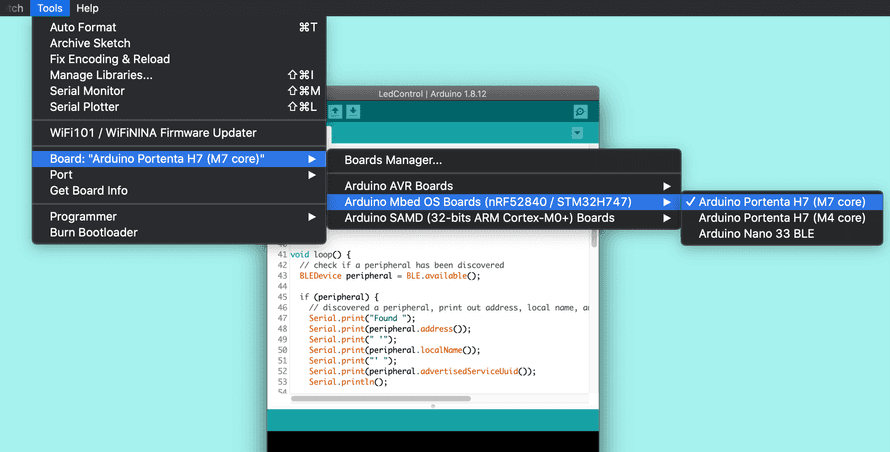
\includegraphics[width=0.7\linewidth]{Images/PortentaH7/select-board-h7.png}
							\caption{select-board-h7}
							\label{select-board-h7}
						\end{center}
					\end{figure}
					
				Choose the Port where your Portenta is connected to and Upload the sketch. Open the Serial Monitor once you have uploaded the code to the board to see debugging messages. If the Bluetooth® Low Energy setup was successful, you should see the message BLE LED Control ready. If something went wrong, you will see the message Starting Bluetooth® Low Energy failed!. In that case update the Arduino BLE library (in the Library Manager) and the board (in the Board Manager) to the latest version and try again. ~\ref{select-port}
				
					\begin{figure}
						\begin{center}
							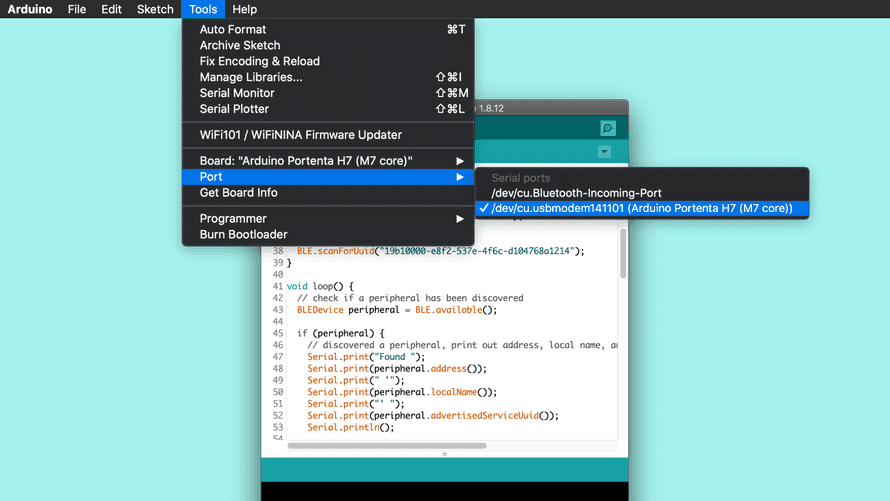
\includegraphics[width=0.7\linewidth]{Images/PortentaH7/select-port.png}
							\caption{select-port}
							\label{select-port}
						\end{center}
					\end{figure}
					
				\item \textbf{5.  Connect an External Device :} On your mobile device install nRF Connect or an equivalent app that allows for Bluetooth® Low Energy connections. We will refer to nRF Connect for the rest of this tutorial. ~\ref{NRF-Connect}
					\begin{figure}
						\begin{center}
							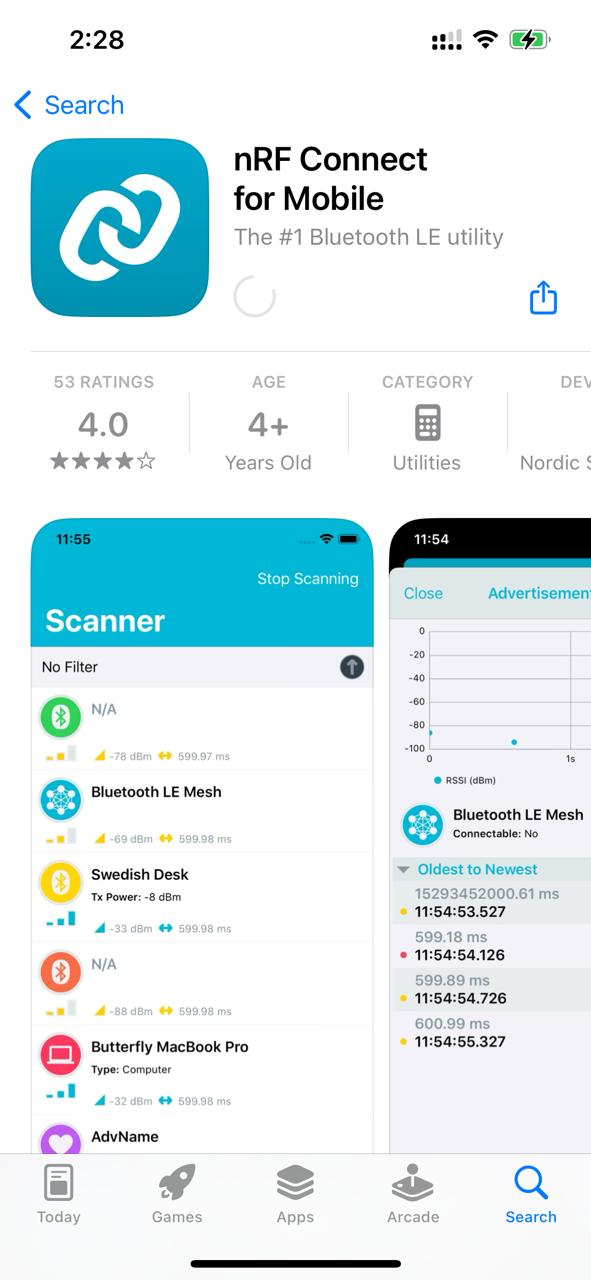
\includegraphics[width=0.7\linewidth]{Images/PortentaH7/NRF-Connect.jpg}
							\caption{NRF-Connect}
							\label{NRF-Connect}
						\end{center}
					\end{figure}
				Once you have downloaded the nRF application on your mobile device, look for your Portenta in the device list. You may filter the list by "Portenta" to easierly find your board in case you are using nRF Connect.
				
				\item When you find your board in the list tap "Connect".
				\item Navigate to the "Services" screen and tap the arrow up button.
				\item Switch to "Bool" type and move the toggle to "True". Confirm the dialog with a tap on "Write" and you should see the built-in LED turned on. If you do the same procedure again but setting the toggle switch to "False", it will turn off the LED. ~\ref{Bluetooth-scan}
					\begin{figure}
						\begin{center}
							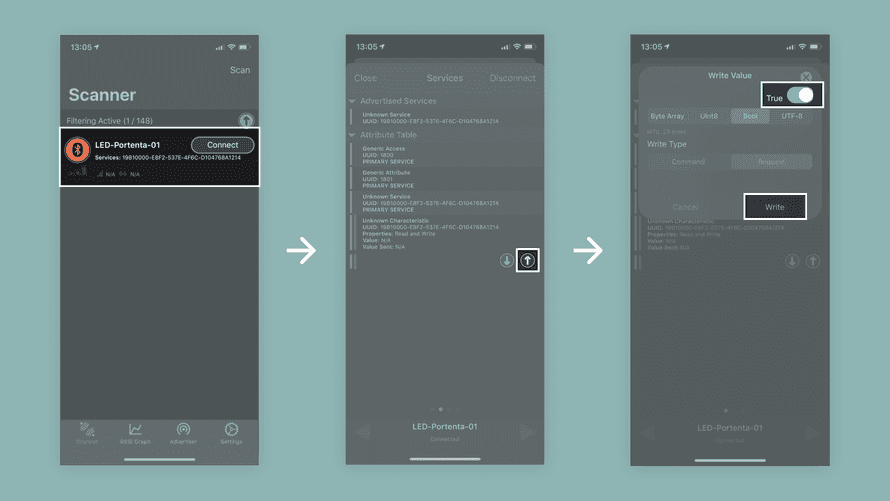
\includegraphics[width=0.7\linewidth]{Images/PortentaH7/Bluetooth-scan.png}
							\caption{Bluetooth-scan}
							\label{Bluetooth-scan}
						\end{center}
					\end{figure}
				\item \textbf{6. Conclusion:} This example shows how to connect and control the built-in LED using a Bluetooth® Low Energy connection. You have learned how a simple Bluetooth® Low Energy connection between your Portenta and your cell phone, which has basic communication abilities between the two devices, works. ~\ref{NRF-Connect}	
				
			\end{itemize}
		

		



\section{First Step with PortentaH7:}
	
	\subsection{Setting Up Portenta H7 For Arduino:}
		This Example teaches you how to set up the board, how to configure your computer and how to run the classic Arduino blink example to verify if the configuration was successful. ~\ref{PortentaH7-connection} \cite{portentaSetup:2024}
	\subsection{Goals:}
		\begin{itemize}
			\item About the Arduino and Mbed operating system (Mbed OS) stack
			\item Installing the Mbed library
			\item Controlling the built in LED on the Portenta board
		\end{itemize}
	\subsection{Instructions:}
		\begin{itemize}
			\item \textbf{Configuring the Development Environment:} In this section, we will guide you through a step-by-step process of setting up your Portenta board for running an Arduino Sketch that blinks the built-in RGB LED.
			\item \textbf{The Basic Setup:} Let's begin by Plug-in your Portenta to your computer using the appropriate USB-C® cable. Next, open your IDE and make sure that you have the right version of the Arduino IDE downloaded on to your computer.
				\begin{figure}
					\begin{center}
						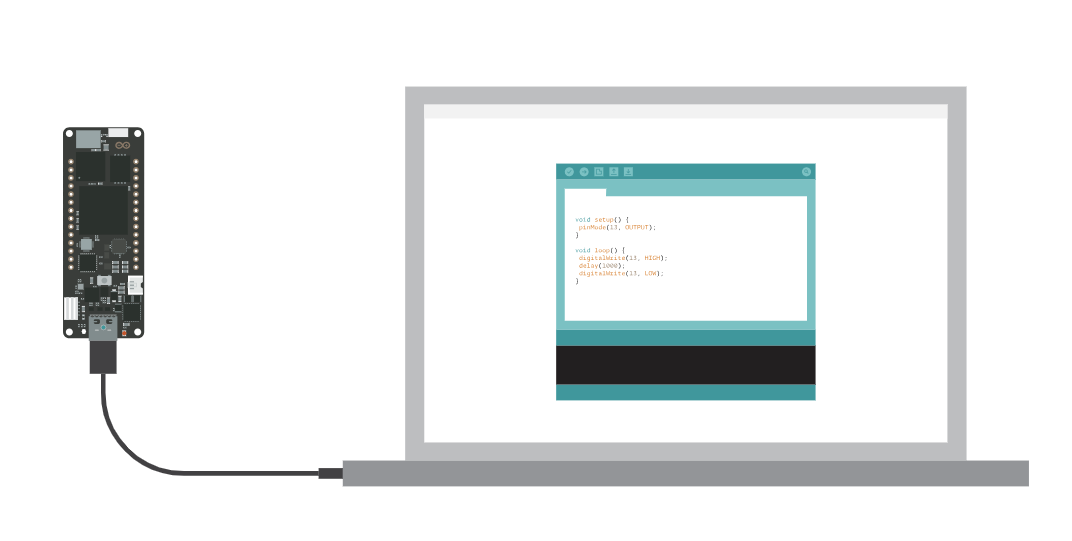
\includegraphics[width=0.7\linewidth]{Images/PortentaH7/PortentaH7-connection.png}
						\caption{PortentaH7-connection}
						\label{PortentaH7-connection}
					\end{center}
				\end{figure}
			\item \textbf{Adding the Portenta to the List of Available Boards:} In your Arduino IDE, open the board manager and search for "portenta". Find the Arduino mbed-enabled Boards library and click on "Install" to install the latest version of the mbed core (1.2.3 at the time of writing this tutorial). ~\ref{Portentaport}
				\begin{figure}
					\begin{center}
						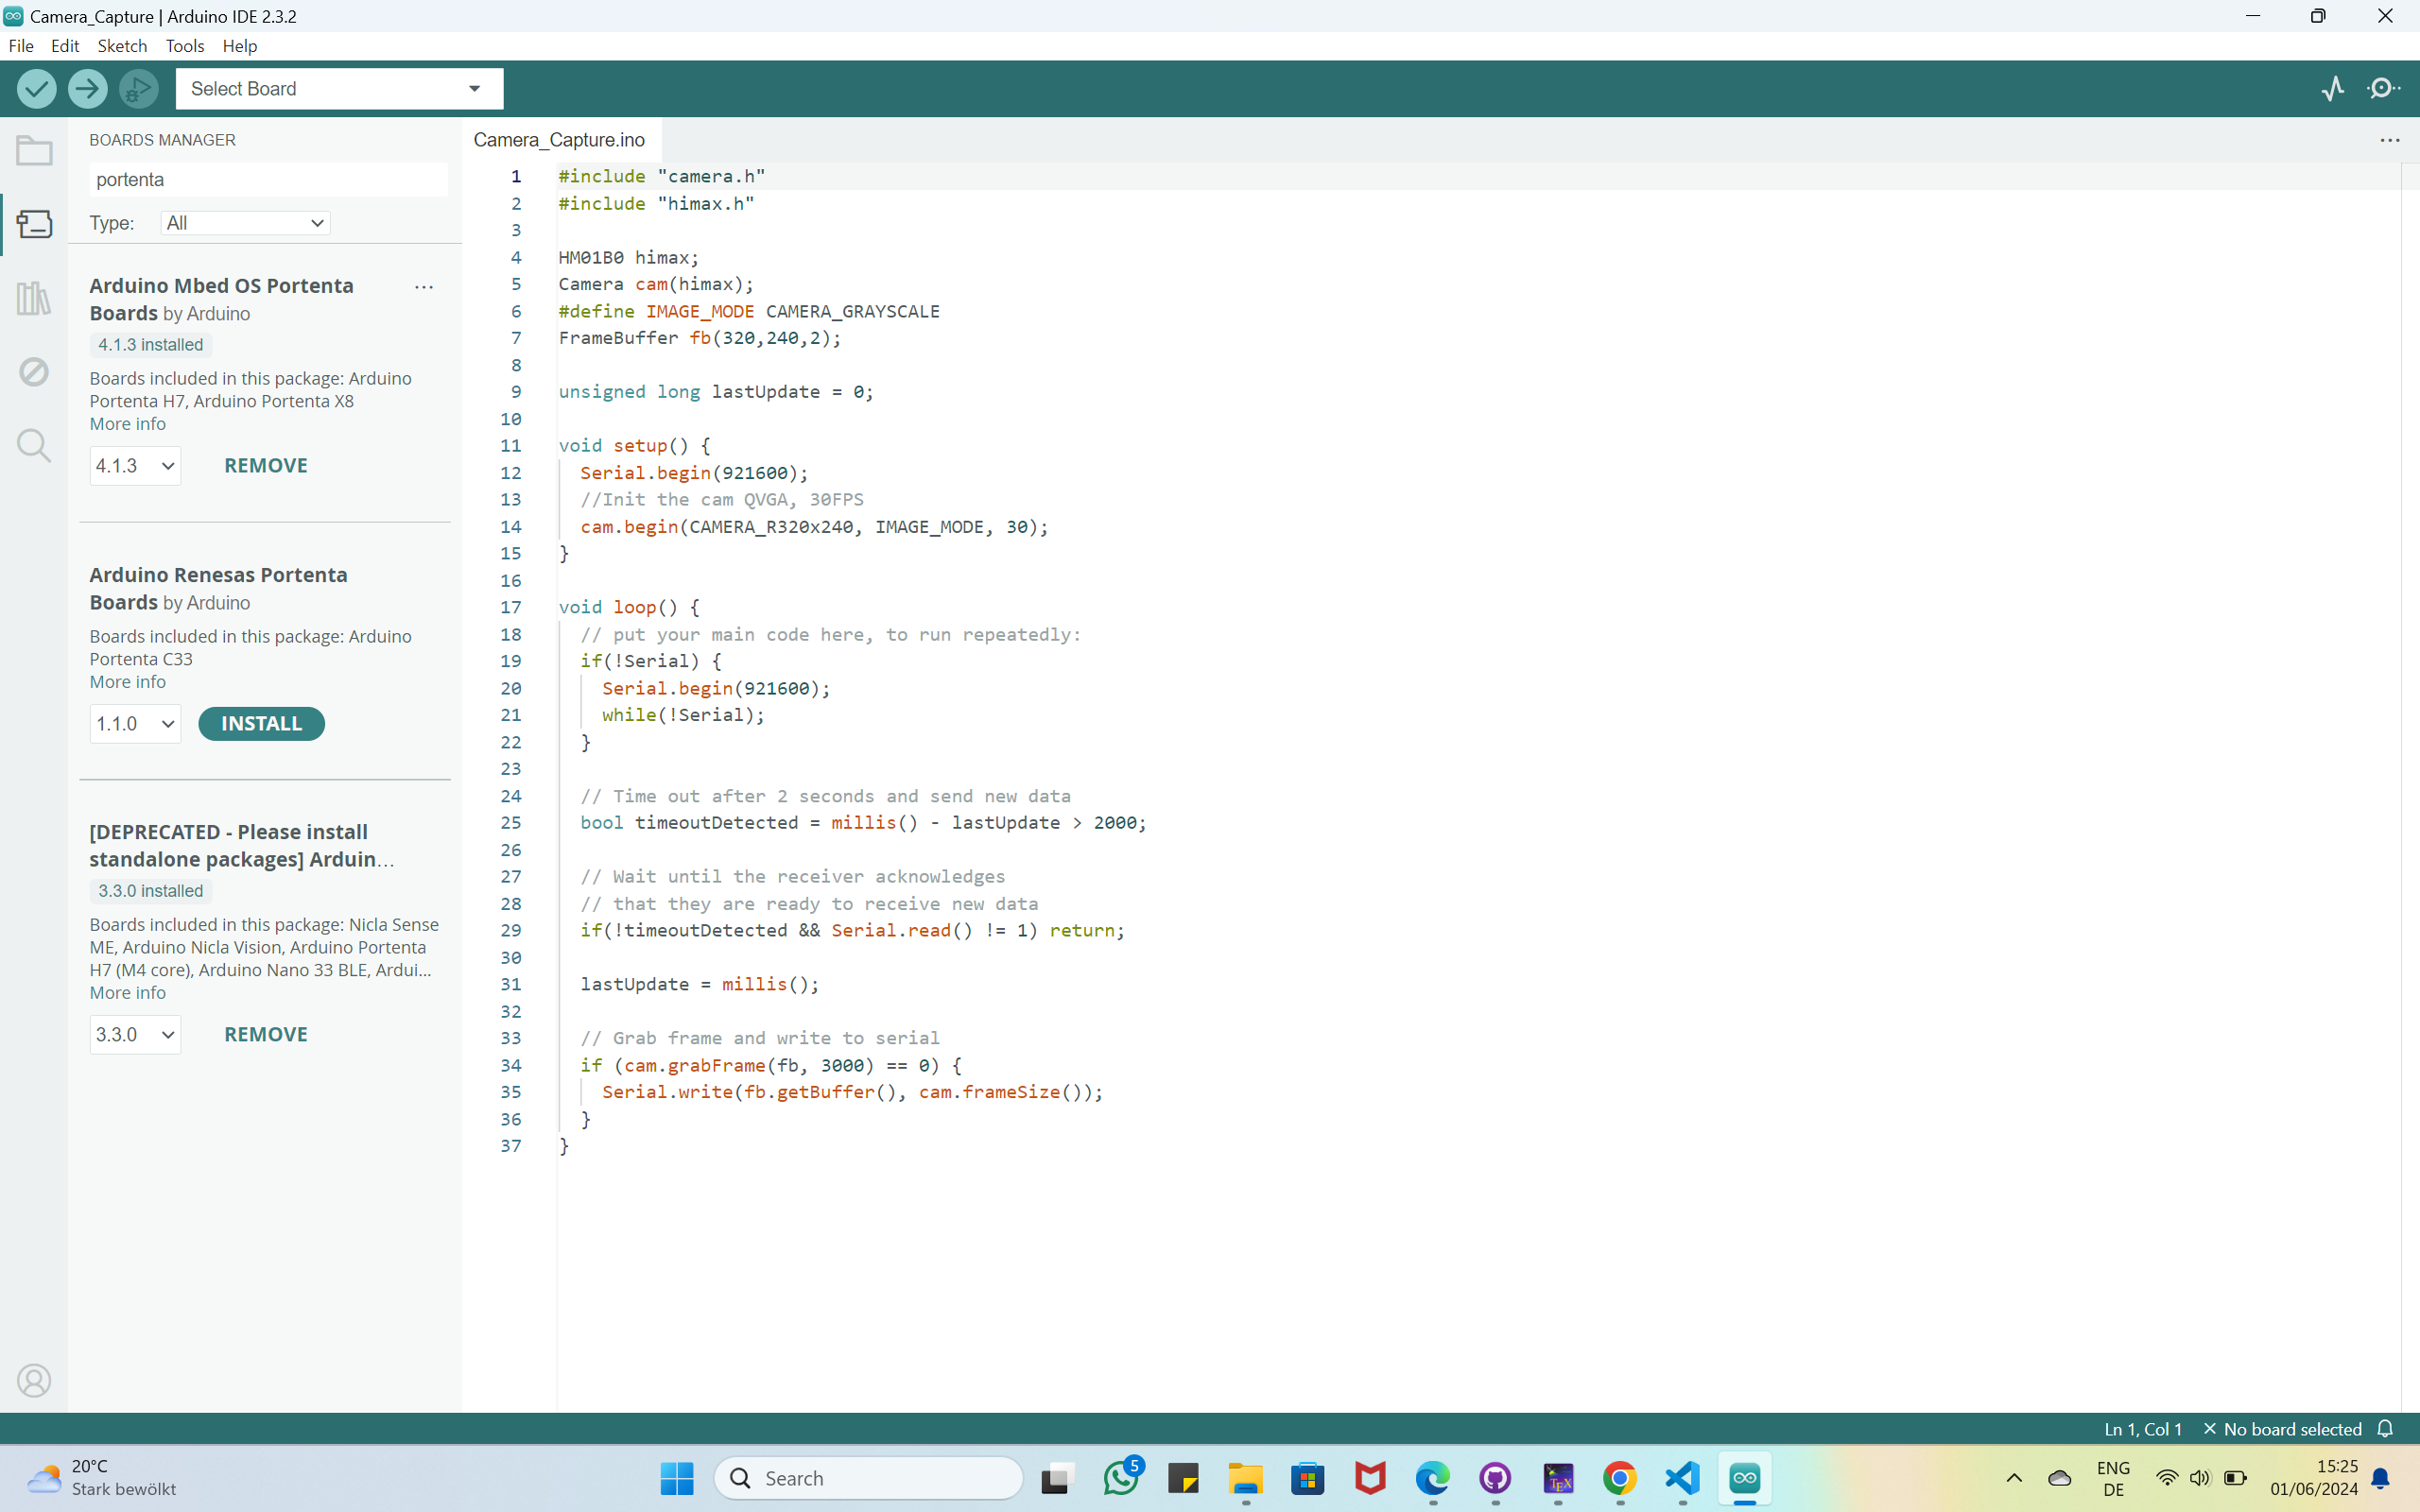
\includegraphics[width=0.7\linewidth]{Images/PortentaH7/Portentaport.png}
						\caption{Portentaport}
						\label{Portentaport}
					\end{center}
				\end{figure}
				
			\item \textbf{Uploading the Classic Blink Sketch:} Let's program the Portenta with the classic blink example to check if the connection to the board works. 
			
					\begin{lstlisting}
						// the setup function runs once when you press reset or power the board
						void setup() {
							// initialize digital pin LED_BUILTIN as an output.
							pinMode(LED_BUILTIN, OUTPUT);
							digitalWrite(LED_BUILTIN, HIGH); // turn the LED off after being turned on by pinMode()
						}
						
						// the loop function runs over and over again forever
						void loop() {
							digitalWrite(LED_BUILTIN, LOW); // turn the LED on (LOW is the voltage level)
							delay(1000); // wait for a second
							digitalWrite(LED_BUILTIN, HIGH); // turn the LED off by making the voltage HIGH
							delay(1000); // wait for a second
						}   
								
					\end{lstlisting}
			
		\end{itemize}
		
	\subsection{Conclusion:}
		You have now configured your Portenta board to run Arduino sketches. Along with that you gained an understanding of how the Arduino Core runs on top of Mbed OS.
		
		


	
=======
%%%%%%%%%%%%%%%%%%%%%%%%
%
% $Autor: Wings $
% $Datum: 2020-07-24 09:05:07Z $
% $Pfad: GDV/Vortraege/latex - Ausarbeitung/Kapitel/Einleitung.tex $
% $Version: 4732 $
%
%%%%%%%%%%%%%%%%%%%%%%%%

\chapter{PortentaH7}
	The PortentaH7 is a high-performance microcontroller board developed by Arduino. It is designed to cater to professional applications, offering robust computing power, advanced features, and versatility. Here are some key aspects of the PortentaH7:
	
	Within the H7 family, there are two variants; H7 Lite and H7 Lite Connected. All the three boards and their differences are presented in this datasheet.
	
	\textbf{Target Areas}: 
	Laboratory equipment, Computer vision
	
	\begin{figure}
		\begin{center}
			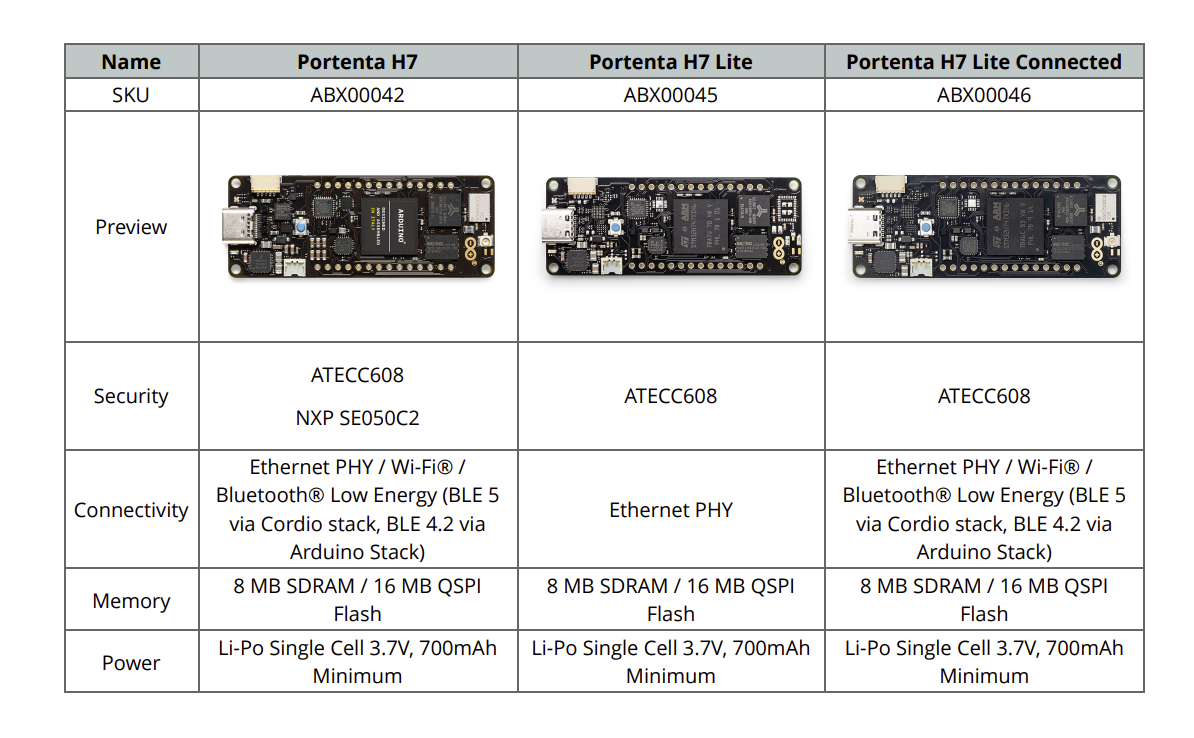
\includegraphics[width=0.7\linewidth]{Images/PortentaH7/TypesofPortentaH7.png}
			\caption{Types of PortentaH7}
			\label{Types}
		\end{center}
	\end{figure}
	
\section{Key Features:}

\textbf{Dual-core Processor:}

\begin{itemize}
	\item Cortex-M7: Runs at up to 480 MHz.
	\item Cortex-M4: Runs at up to 240 MHz.
	\item These cores can operate simultaneously, allowing for efficient parallel processing and real-time application execution.
\end{itemize}

\textbf{Memory:}
\begin{itemize}
	\item RAM: 1 MB of SRAM and 16 MB of SDRAM.
	\item Flash Storage: 8 MB.
\end{itemize}

\textbf{Connectivity:}
\begin{itemize}
	\item $<$ Built-in GPU for handling advanced graphical interfaces. 
	\item $<$ Supports an external display through a dedicated connector.
\end{itemize}

\textbf{Security:}
\begin{itemize}
	\item Hardware cryptography support for secure applications.
	\item Secure boot and secure firmware updates.
\end{itemize}

\textbf{Expansion Options:}
\begin{itemize}
	\item Compatible with Arduino MKR and \textbf{Portenta Vision Shield.}
	\item High-density connectors for custom hardware extensions.
\end{itemize}

\textbf{Operating Systems:}
\begin{itemize}
	\item Capable of running high-level OS like Arm Mbed OS or real-time operating systems (RTOS).
	\item Compatible with Arduino programming environment and libraries.
\end{itemize}

\textbf{Power Management:}
\begin{itemize}
	\item Multiple power supply options: USB-C, Li-Po battery, or external sources.
	\item Low power modes for energy-efficient applications.
\end{itemize}

\textbf{Applications:} \newline
	The Portenta H7 is suitable for a wide range of professional applications, including but not limited to:
\begin{itemize}
	\item \textbf{Industrial IoT:} Real-time monitoring, data acquisition, and control systems.
	\item \textbf{Edge Computing:} Local data processing and decision-making.
	\item \textbf{AI and Machine Learning:} On-device inference and analytics.
	\item \textbf{Robotics:} Advanced motor control and sensor integration.
	\item \textbf{Smart Devices:} Connected appliances, home automation, and wearables.
\end{itemize}

\section{Onboard Sensors with Examples}

	\subsection{Murata 1DX Bluetooth® 5.1}
		The onboard Bluetooth® module of the Portenta H7 offers low energy Bluetooth® functionality, in order to provide the board with the flexibility to be easily connected to devices which also support Bluetooth® Low Energy, such as the Arduino Nano 33 IoT or most modern smartphones. Compared to classic Bluetooth®, Low Energy Bluetooth® is intended to provide considerably reduced power consumption and cost while maintaining a similar communication range. \cite{bluetoothPortentaH7:2024}
		
		\subsubsection{Overview}
			In this Example we will enable low energy Bluetooth® on the Portenta H7 to allow an external Bluetooth® device to control the built-in LED either by turning it on or off.
	
		\subsubsection{Goals}
			\begin{itemize}
				\item Enabling Bluetooth® Low Energy connectivity on the Portenta H7.
				\item Connecting the Portenta to an external Bluetooth® Low Energy Mobile Application (In this case nRF Connect by Nordic Semiconductor).
			\end{itemize}
			
		\subsubsection{Required Hardware and Software}
			\begin{itemize}
				\item Portenta H7 (ABX00042) or Portenta H7 Lite Connected (ABX00046)
				\item USB-C® cable (either USB-A to USB-C® or USB-C® to USB-C®)
				\item Arduino IDE 1.8.13+ or Arduino Pro IDE 0.0.4+
				\item Mobile device, phone or tablet
				\item nRFconnect or equivalent tool downloaded on your mobile device: nRF Connect for iOS or nRF Connect for android
			\end{itemize}
			
		\subsubsection{Instructions}
			\begin{itemize}
				\item \textbf{Configuring the Development Environment:} To communicate with the Portenta H7 via Bluetooth®, you need to upload a pre-built sketch that starts a Bluetooth® network and allows your mobile device, which will be used to control the LEDs, to connect to it. The sketch uses the ArduinoBLE Library that enables the Bluetooth® Low Energy module and handles important functions, such as scanning, connecting and interacting with services provided by other devices. You will also be using a third party application (e.g. nRF Connect), running on your mobile device in order to connect your device to the board and help you control the built-in LED. ~\ref{Bluetooth-portentaH7}
					\begin{figure}
						\begin{center}
							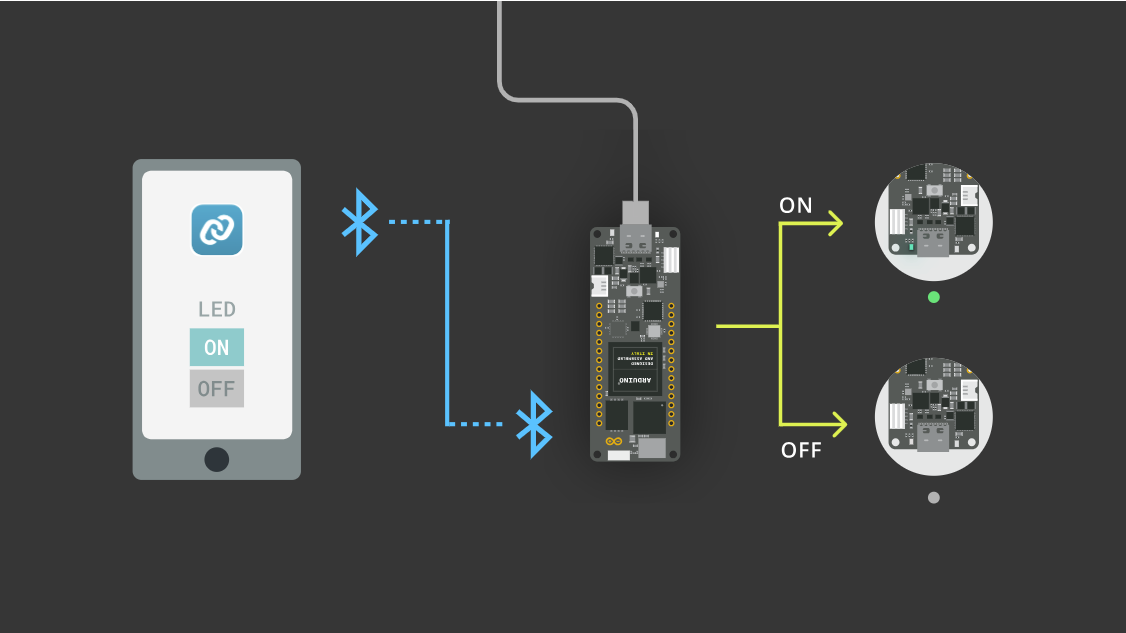
\includegraphics[width=0.7\linewidth]{Images/PortentaH7/Bluetooth-portentaH7.png}
							\caption{Bluetooth-portentaH7}
							\label{Bluetooth-portentaH7}
						\end{center}
					\end{figure}
					
				\item \textbf{1. The Basic Setup:} Begin by plugging in your Portenta board to the computer using a USB-C® cable and open the Arduino IDE. If this is your first time running Arduino sketch files on the board, we suggest you check out how to set up the Portenta H7 for Arduino before you proceed.
					\begin{figure}
						\begin{center}
							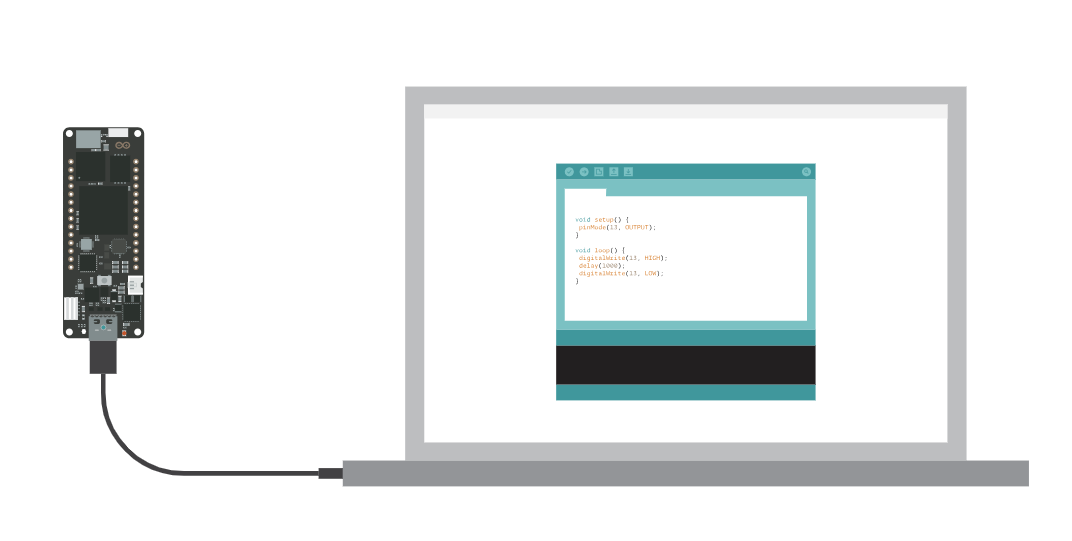
\includegraphics[width=0.7\linewidth]{Images/PortentaH7/PortentaH7-connection.png}
							\caption{PortentaH7-connection}
							\label{PortentaH7-connection}
						\end{center}
					\end{figure}
				
				\item \textbf{2. Install the ArduinoBLE Library:} You will need to install the ArduinoBLE library in the Arduino IDE you are using. To install the library go to : Tools > Manage Libraries... type ArduinoBLE and click Install. Make sure you install ArduinoBLE version 1.1.3 or higher. ~\ref{Bluetooth-Library}
					\begin{figure}
						\begin{center}
							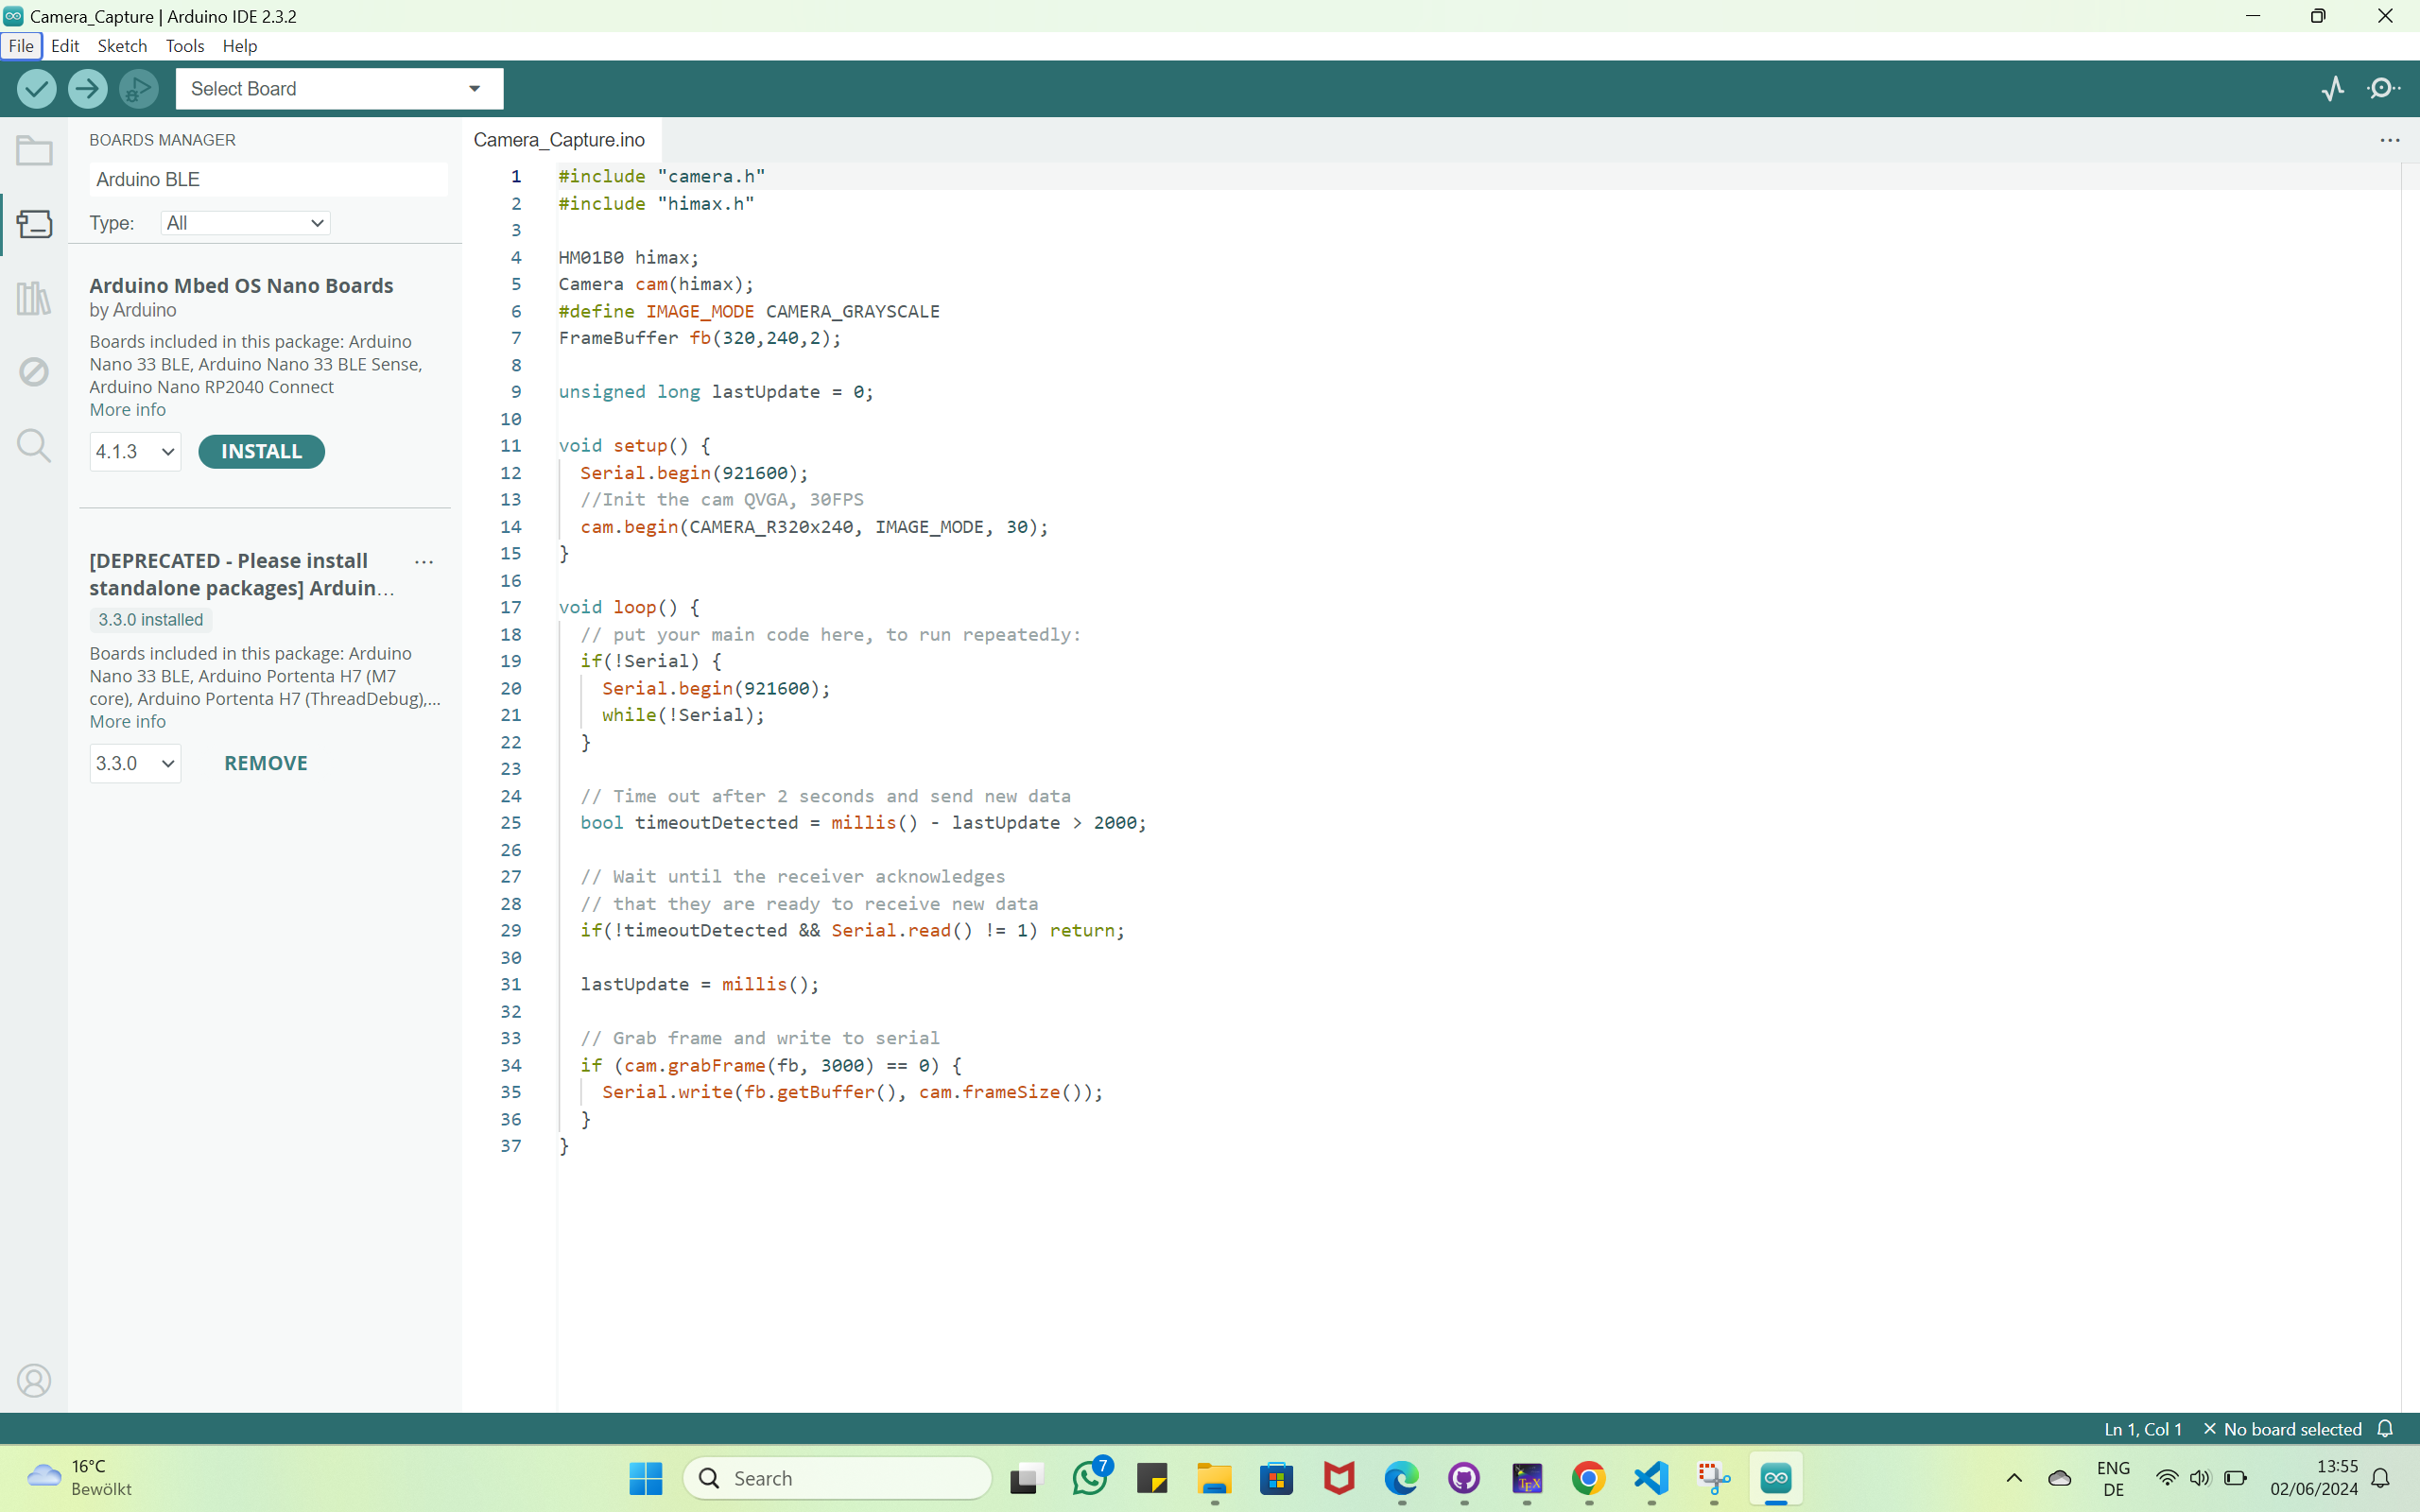
\includegraphics[width=0.7\linewidth]{Images/PortentaH7/Bluetooth-Library.png}
							\caption{Bluetooth-Library}
							\label{Bluetooth-Library}
						\end{center}
					\end{figure}
				
				\item \textbf{3. Create the Bluetooth® Low Energy Sketch:} Let's program the Portenta with the following example sketch. If the Bluetooth® Low Energy module has been initialized correctly, you will see the blue LED lighting up for one second after uploading the sketch. If it fails, you will see the red LED lighting up instead. Copy and paste the following code into a new sketch in your IDE or download it from Arduino-Pro-Tutorials in the Arduino IDE and open it from: Examples > Arduino-Pro-Tutorials > BLE Connectivity on Portenta H7 > PortentaBLE 
					\begin{lstlisting}
						#include <ArduinoBLE.h>
						
						BLEService ledService("19b10000-e8f2-537e-4f6c-d104768a1214");
						
						// Bluetooth Low Energy LED Switch Characteristic - custom 128-bit UUID, read and writable by central
						BLEByteCharacteristic switchCharacteristic("19b10000-e8f2-537e-4f6c-d104768a1214", BLERead | BLEWrite);
						
						const int ledPin = LED-BUILTIN; // Pin to use for the LED
						
						void setup() {
							Serial.begin(9600);
							//while (!Serial);   // Uncomment to wait for serial port to connect.
							
							// Set LED pin to output mode
							pinMode(ledPin, OUTPUT);
							digitalWrite(ledPin, HIGH);
							
							// Begin initialization
							if (!BLE.begin()) {
								Serial.println("Starting Bluetooth Low Energy failed!");
								digitalWrite(LEDR, LOW);
								delay(1000);
								digitalWrite(LEDR, HIGH);
								
								// Stop if Bluetooth Low Energy couldn't be initialized.
								while (1);
							}
							
							// Set advertised local name and service UUID:
							BLE.setLocalName("LED-Portenta-01");
							BLE.setAdvertisedService(ledService);
							
							// Add the characteristic to the service
							ledService.addCharacteristic(switchCharacteristic);
							
							// Add service
							BLE.addService(ledService);
							
							// Set the initial value for the characeristic:
							switchCharacteristic.writeValue(0);
							
							// start advertising
							BLE.advertise();
							digitalWrite(LEDB, LOW);
							delay(1000);
							digitalWrite(LEDB, HIGH);
							Serial.println("BLE LED Control ready");
						}
						
						void loop() {
							// Listen for Bluetooth Low Energy peripherals to connect:
							BLEDevice central = BLE.central();
							
							// If a central is connected to peripheral:
							if (central) {
								Serial.print("Connected to central: ");
								// Print the central's MAC address:
								Serial.println(central.address());
								digitalWrite(LEDB, HIGH);
								delay(100);
								digitalWrite(LEDB, LOW);
								delay(100);
								digitalWrite(LEDB, HIGH);
								
								// While the central is still connected to peripheral:
								while (central.connected()) {
									// If the remote device wrote to the characteristic,
									// Use the value to control the LED:
									if (switchCharacteristic.written()) {
										if (switchCharacteristic.value()) {   // Any value other than 0
											Serial.println("LED on");
											digitalWrite(ledPin, LOW);          // Will turn the Portenta LED on
										} else {                             
											Serial.println("LED off");
											digitalWrite(ledPin, HIGH);         // Will turn the Portenta LED off          
										}
									}
								}
								
								// When the central disconnects, print it out:
								Serial.print("Disconnected from central: ");
								Serial.println(central.address());    
								digitalWrite(LEDB, HIGH);
								delay(100);
								digitalWrite(LEDB, LOW);
								delay(100);
								digitalWrite(LEDB, HIGH);
							}
						}    
								
					\end{lstlisting}
					
					In this example, you use a pre-defined Bluetooth number code pre-setup for controlling a device's LED. This code can also be referred to as GATT codes, which define how two Bluetooth® low energy devices transfer data. Once a connection is established with a device, its respective GATT code, which is a 16 bit identifier, is stored in a lookup table for future reference.
					
					These GATT codes are very long, but, in this example, it is always the same code:
					\begin{lstlisting}
						BLEService ledService("19b10000-e8f2-537e-4f6c-d104768a1214"); // BLE LED Service
					\end{lstlisting}	
					
				\item \textbf{4. Upload the Sketch:} Double press the reset button so the built-in LED is slowly pulsing green. Then, select your board in the menu: Tools > Board > Arduino Portenta H7 (M7 core) ~\ref{select-board-h7}
					\begin{figure}
						\begin{center}
							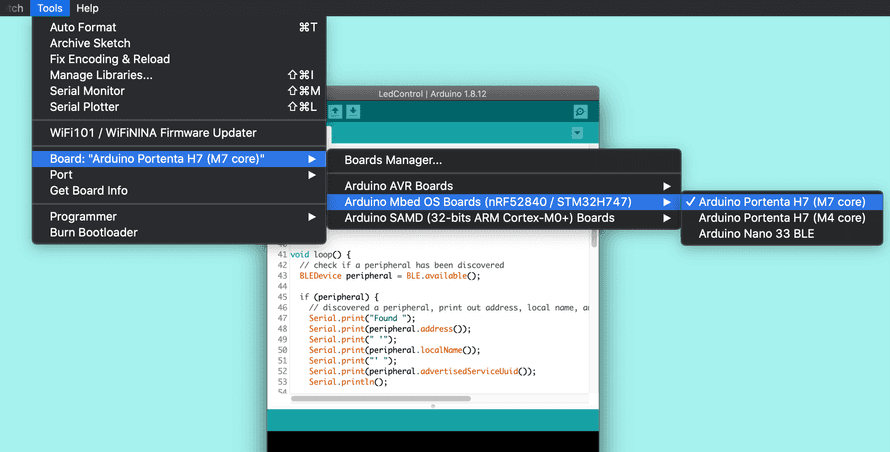
\includegraphics[width=0.7\linewidth]{Images/PortentaH7/select-board-h7.png}
							\caption{select-board-h7}
							\label{select-board-h7}
						\end{center}
					\end{figure}
					
				Choose the Port where your Portenta is connected to and Upload the sketch. Open the Serial Monitor once you have uploaded the code to the board to see debugging messages. If the Bluetooth® Low Energy setup was successful, you should see the message BLE LED Control ready. If something went wrong, you will see the message Starting Bluetooth® Low Energy failed!. In that case update the Arduino BLE library (in the Library Manager) and the board (in the Board Manager) to the latest version and try again. ~\ref{select-port}
				
					\begin{figure}
						\begin{center}
							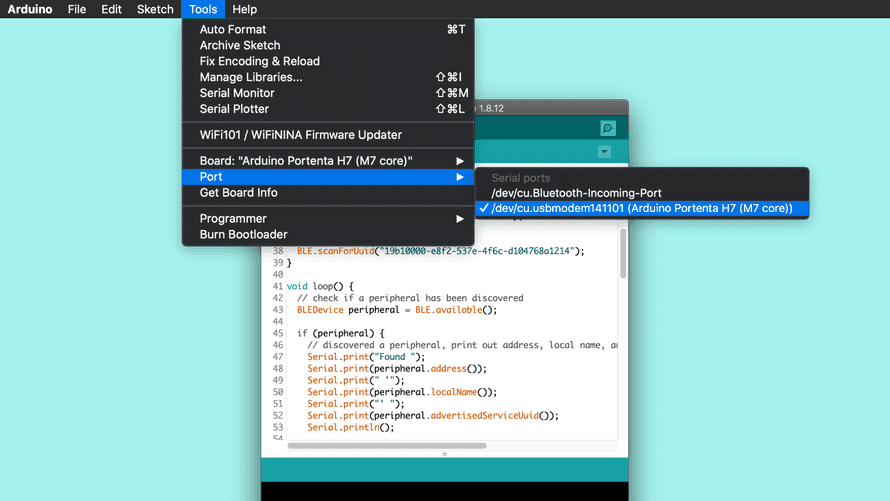
\includegraphics[width=0.7\linewidth]{Images/PortentaH7/select-port.png}
							\caption{select-port}
							\label{select-port}
						\end{center}
					\end{figure}
					
				\item \textbf{5.  Connect an External Device :} On your mobile device install nRF Connect or an equivalent app that allows for Bluetooth® Low Energy connections. We will refer to nRF Connect for the rest of this tutorial. ~\ref{NRF-Connect}
					\begin{figure}
						\begin{center}
							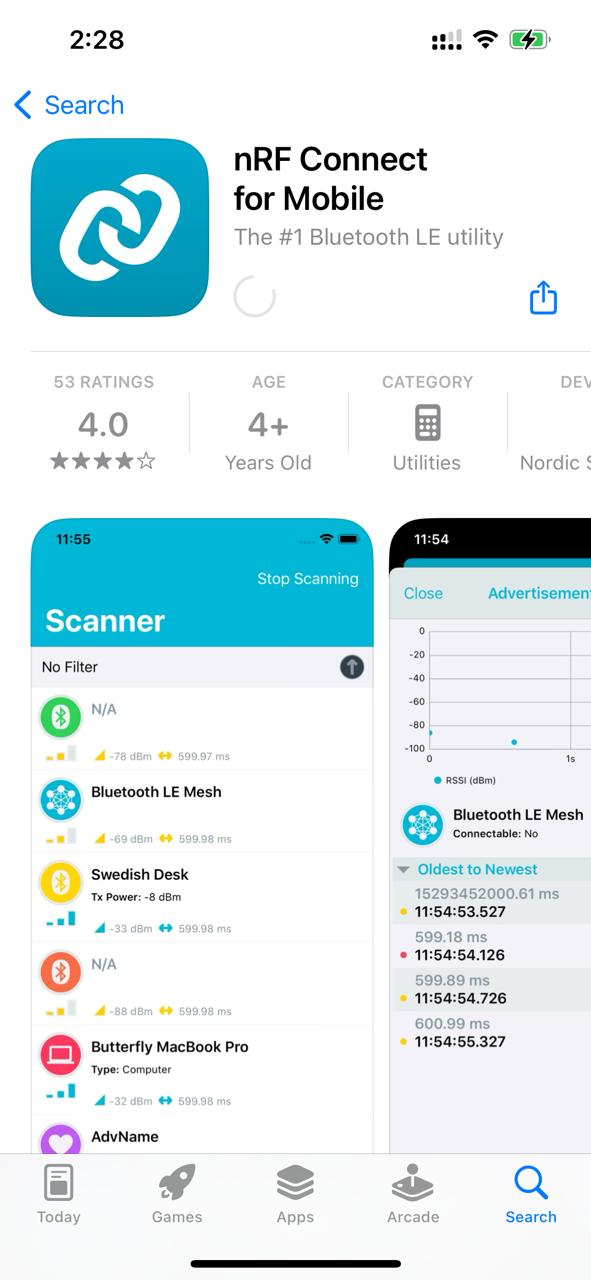
\includegraphics[width=0.7\linewidth]{Images/PortentaH7/NRF-Connect.jpg}
							\caption{NRF-Connect}
							\label{NRF-Connect}
						\end{center}
					\end{figure}
				Once you have downloaded the nRF application on your mobile device, look for your Portenta in the device list. You may filter the list by "Portenta" to easierly find your board in case you are using nRF Connect.
				
				\item When you find your board in the list tap "Connect".
				\item Navigate to the "Services" screen and tap the arrow up button.
				\item Switch to "Bool" type and move the toggle to "True". Confirm the dialog with a tap on "Write" and you should see the built-in LED turned on. If you do the same procedure again but setting the toggle switch to "False", it will turn off the LED. ~\ref{Bluetooth-scan}
					\begin{figure}
						\begin{center}
							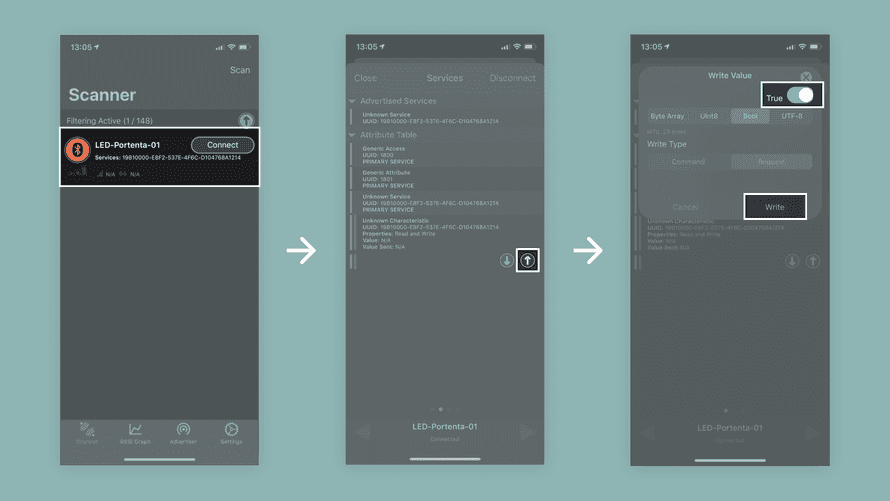
\includegraphics[width=0.7\linewidth]{Images/PortentaH7/Bluetooth-scan.png}
							\caption{Bluetooth-scan}
							\label{Bluetooth-scan}
						\end{center}
					\end{figure}
				\item \textbf{6. Conclusion:} This example shows how to connect and control the built-in LED using a Bluetooth® Low Energy connection. You have learned how a simple Bluetooth® Low Energy connection between your Portenta and your cell phone, which has basic communication abilities between the two devices, works. ~\ref{NRF-Connect}	
				
			\end{itemize}
		

		



\section{First Step with PortentaH7:}
	
	\subsection{Setting Up Portenta H7 For Arduino:}
		This Example teaches you how to set up the board, how to configure your computer and how to run the classic Arduino blink example to verify if the configuration was successful. ~\ref{PortentaH7-connection} \cite{portentaSetup:2024}
	\subsection{Goals:}
		\begin{itemize}
			\item About the Arduino and Mbed operating system (Mbed OS) stack
			\item Installing the Mbed library
			\item Controlling the built in LED on the Portenta board
		\end{itemize}
	\subsection{Instructions:}
		\begin{itemize}
			\item \textbf{Configuring the Development Environment:} In this section, we will guide you through a step-by-step process of setting up your Portenta board for running an Arduino Sketch that blinks the built-in RGB LED.
			\item \textbf{The Basic Setup:} Let's begin by Plug-in your Portenta to your computer using the appropriate USB-C® cable. Next, open your IDE and make sure that you have the right version of the Arduino IDE downloaded on to your computer.
				\begin{figure}
					\begin{center}
						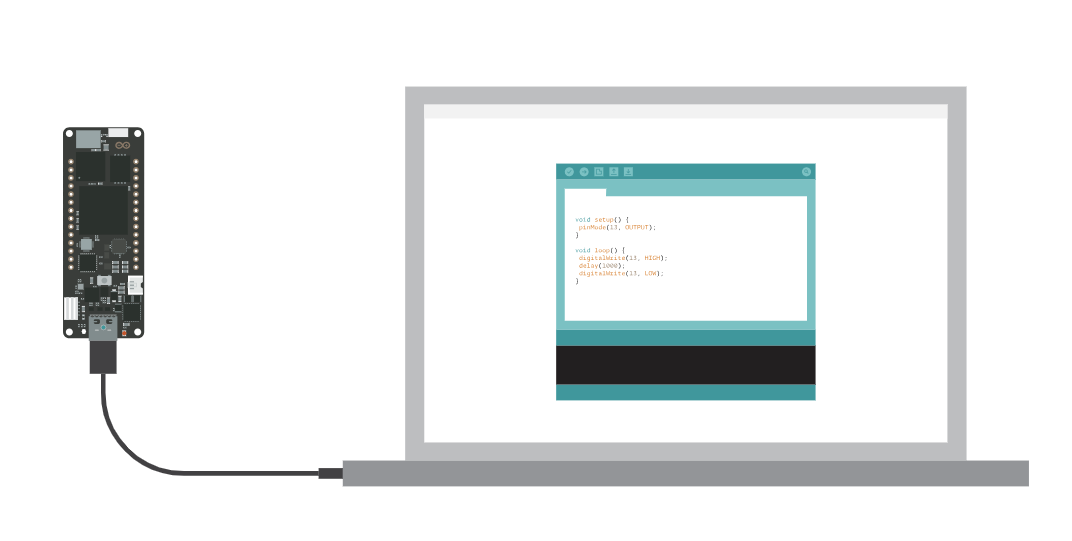
\includegraphics[width=0.7\linewidth]{Images/PortentaH7/PortentaH7-connection.png}
						\caption{PortentaH7-connection}
						\label{PortentaH7-connection}
					\end{center}
				\end{figure}
			\item \textbf{Adding the Portenta to the List of Available Boards:} In your Arduino IDE, open the board manager and search for "portenta". Find the Arduino mbed-enabled Boards library and click on "Install" to install the latest version of the mbed core (1.2.3 at the time of writing this tutorial). ~\ref{Portentaport}
				\begin{figure}
					\begin{center}
						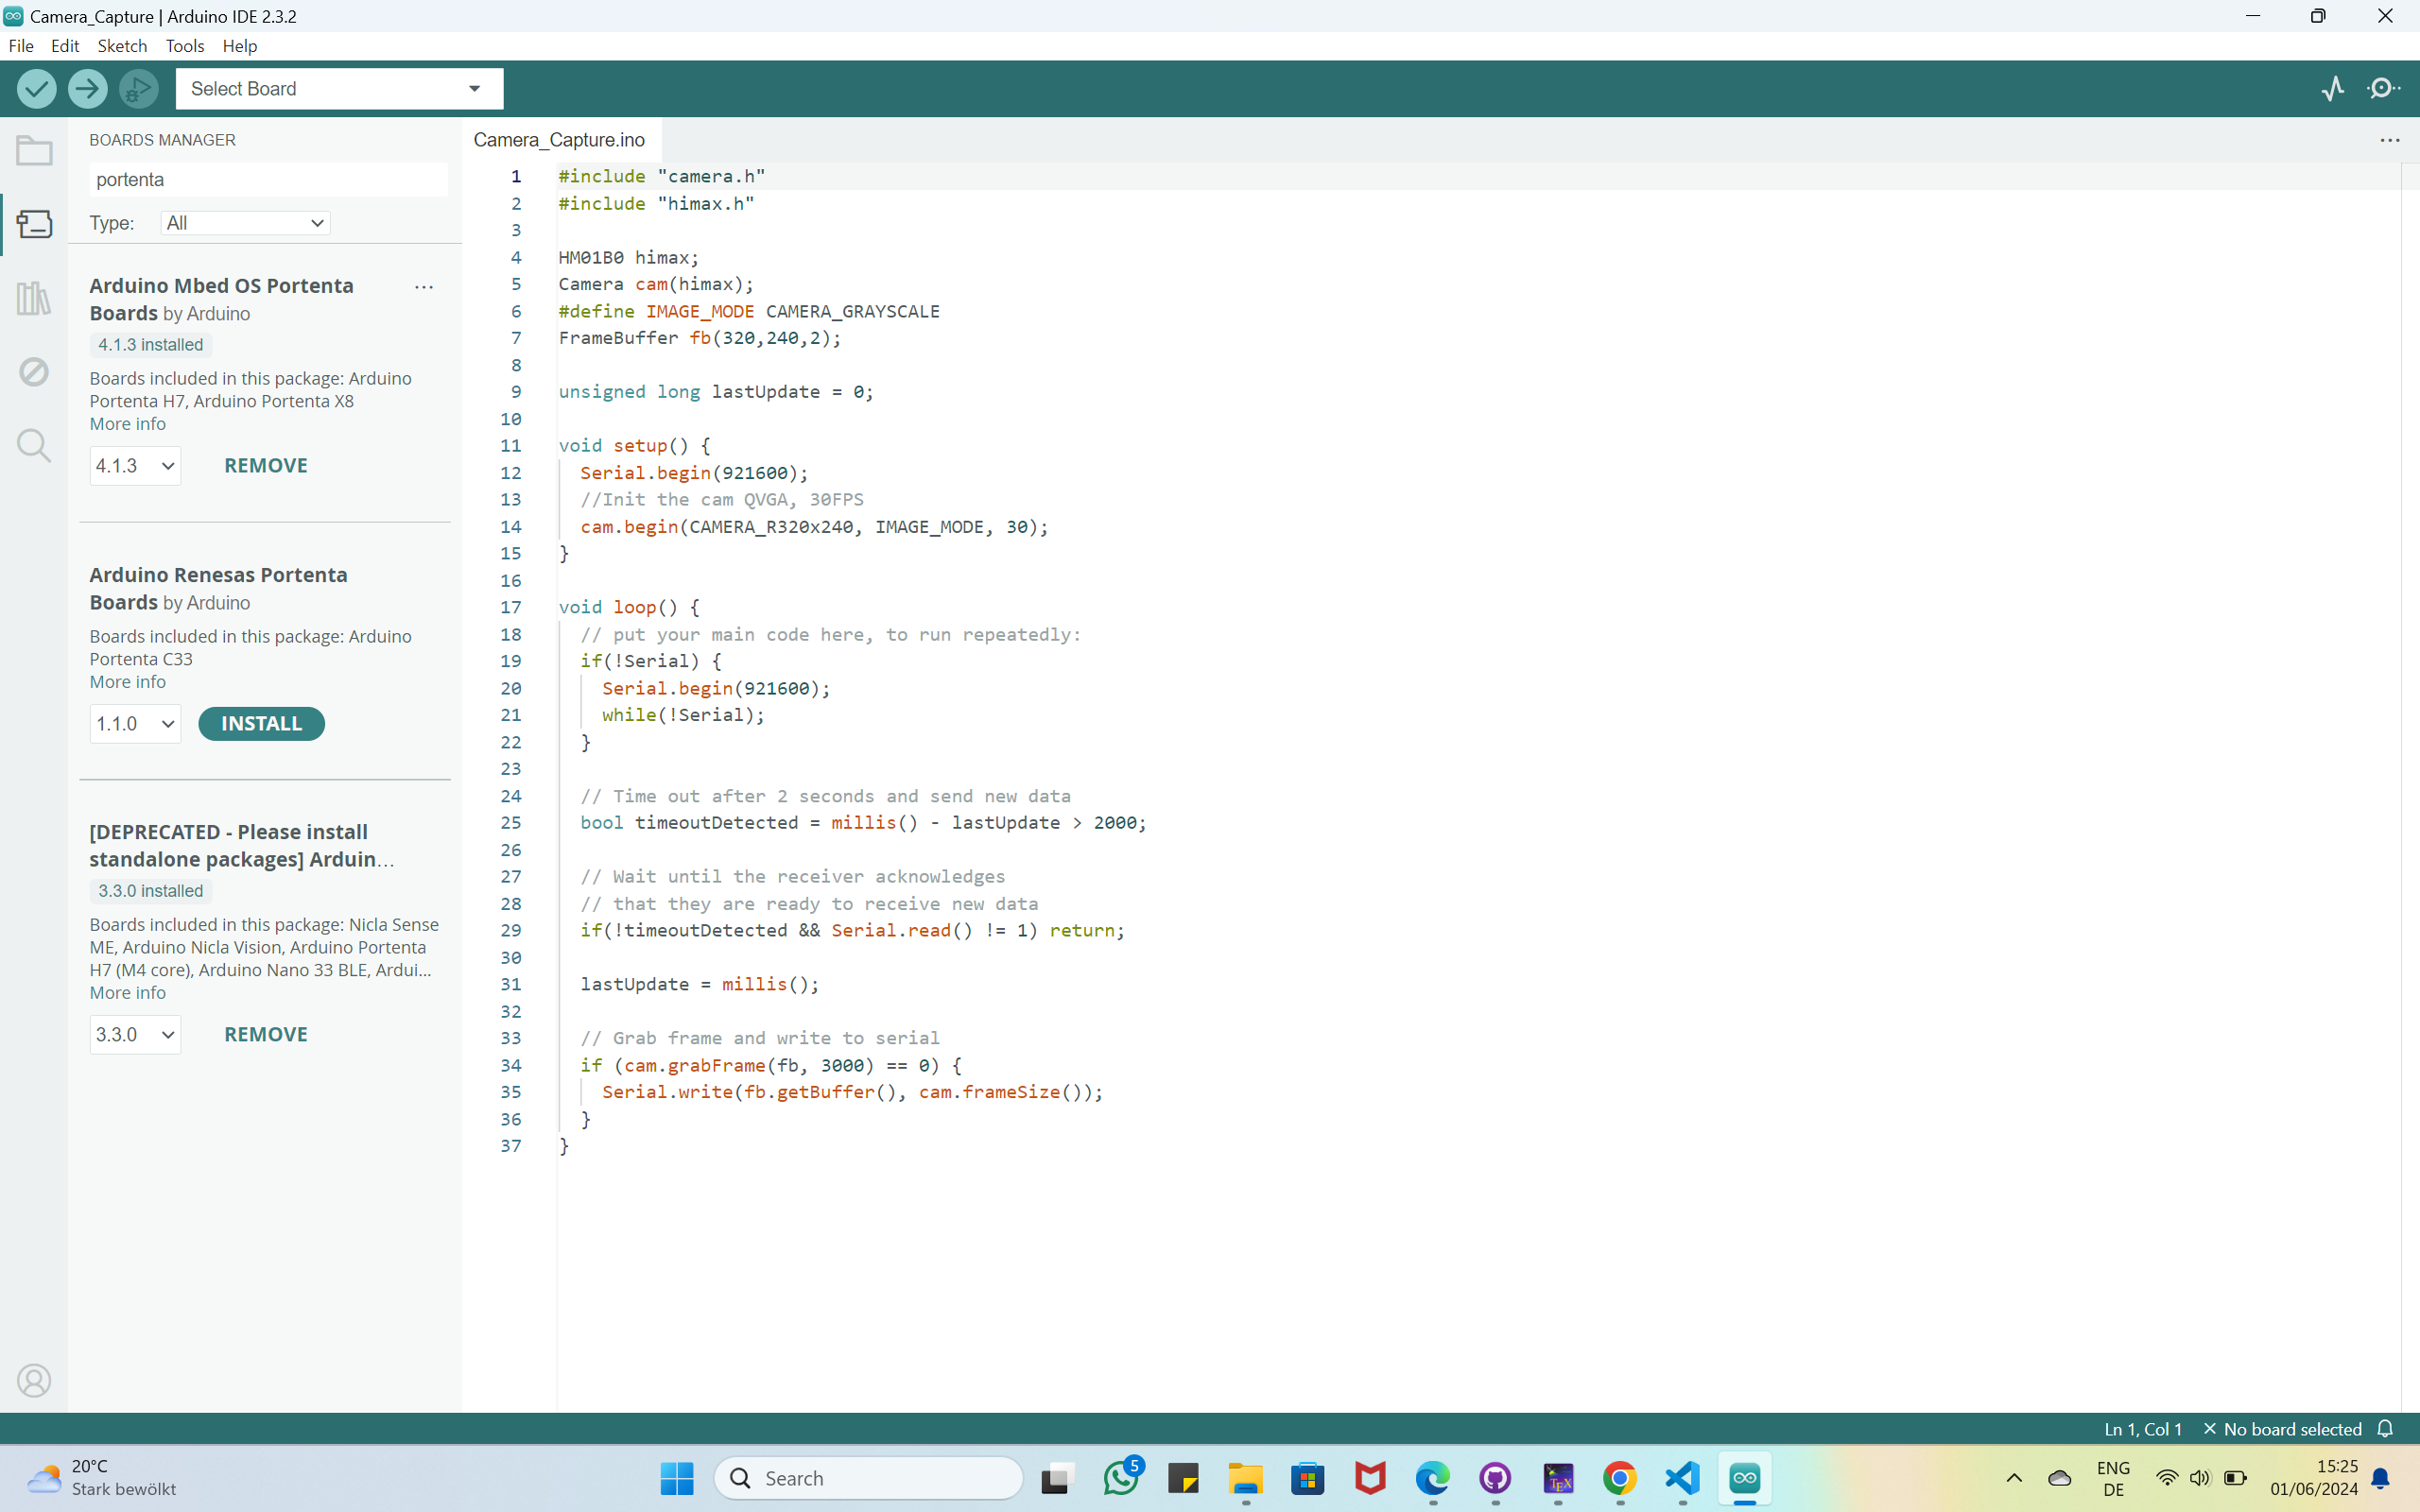
\includegraphics[width=0.7\linewidth]{Images/PortentaH7/Portentaport.png}
						\caption{Portentaport}
						\label{Portentaport}
					\end{center}
				\end{figure}
				
			\item \textbf{Uploading the Classic Blink Sketch:} Let's program the Portenta with the classic blink example to check if the connection to the board works. 
			
					\begin{lstlisting}
						// the setup function runs once when you press reset or power the board
						void setup() {
							// initialize digital pin LED_BUILTIN as an output.
							pinMode(LED_BUILTIN, OUTPUT);
							digitalWrite(LED_BUILTIN, HIGH); // turn the LED off after being turned on by pinMode()
						}
						
						// the loop function runs over and over again forever
						void loop() {
							digitalWrite(LED_BUILTIN, LOW); // turn the LED on (LOW is the voltage level)
							delay(1000); // wait for a second
							digitalWrite(LED_BUILTIN, HIGH); // turn the LED off by making the voltage HIGH
							delay(1000); // wait for a second
						}   
								
					\end{lstlisting}
			
		\end{itemize}
		
	\subsection{Conclusion:}
		You have now configured your Portenta board to run Arduino sketches. Along with that you gained an understanding of how the Arduino Core runs on top of Mbed OS.
		
		





%%%%%%%%%%%%%%%%%%%%%%%%
%
% $Autor: Wings $
% $Datum: 2020-07-24 09:05:07Z $
% $Pfad: GDV/Vortraege/latex - Ausarbeitung/Kapitel/Einleitung.tex $
% $Version: 4732 $
%
%%%%%%%%%%%%%%%%%%%%%%%%

\chapter{Portenta Vision Shield hardware}
\label{Sec:VisionShieldHardware}

The Arduino Portenta Vision Shield is an add-on board providing machine vision capabilities and additional
connectivity to the Portenta family of Arduino boards, designed to meet the needs of industrial automation. The
Portenta Vision Shield connects via a high-density connector to the Portenta boards with minimal hardware and
software setup. ~\ref{VisionShield} \cite{arduinoVisionShield:2024}

\begin{figure}
	\begin{center}
		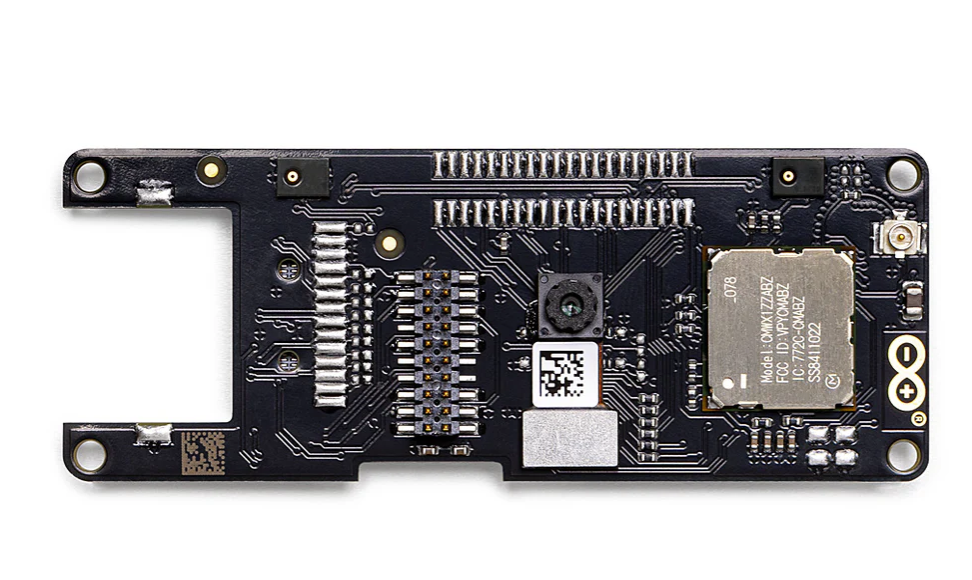
\includegraphics[width=0.7\linewidth]{Images/VisionShield/VisionShield.png}
		\caption{Portenta Vision Shield}
		\label{VisionShield}
	\end{center}
\end{figure}

\section{Features}
	
	\textbf{Himax HM-01B0 Camera Module}
	
	\begin{itemize}
		\item Ultra-Low-Power Image Sensor designed for always-on vision devices and applications
		\item Window, vertical flip, and horizontal mirror readout
		\item Programmable black level calibration target, frame size, frame rate, exposure, analog gain (up to 8x), and digital gain (up to 4x)
		\item Automatic exposure and gain control loop with support for 50 Hz / 60 Hz flicker avoidance
		\item Motion Detection circuit with programmable ROI and detection threshold with digital output to serve as an interrupt
	\end{itemize}
	
	\textbf{Supported Resolutions:}
	\begin{itemize}
		\item QQVGA (160x120) at 15, 30, 60, and 120 FPS 
		\item QVGA (320x240) at 15, 30, and 60 FPS
	\end{itemize}
	
	\textbf{Power:}
	\begin{itemize}
		\item $<$ 1.1 mW QQVGA resolution at 30 FPS
		\item $<$ 2 mW QVGA resolution at 30 FPS 
	\end{itemize}
	
	\textbf{2x MP34DT06JTR MEMS PDM Digital Microphone:}
	\begin{itemize}
		\item AOP = 122.5 dB SPL 
		\item dB signal-to-noise ratio 
		\item Omnidirectional sensitivity 
		\item $-$26 dBFS $\pm$ 1 dB sensitivity 
		\item MIPI 20-pin compatible JTAG Connector 
	\end{itemize}
	
	\textbf{Memory:}
	\begin{itemize}
		\item Micro SD Card Slot
	\end{itemize}

\section{Functional Overview}



\begin{figure}
	\begin{center}
		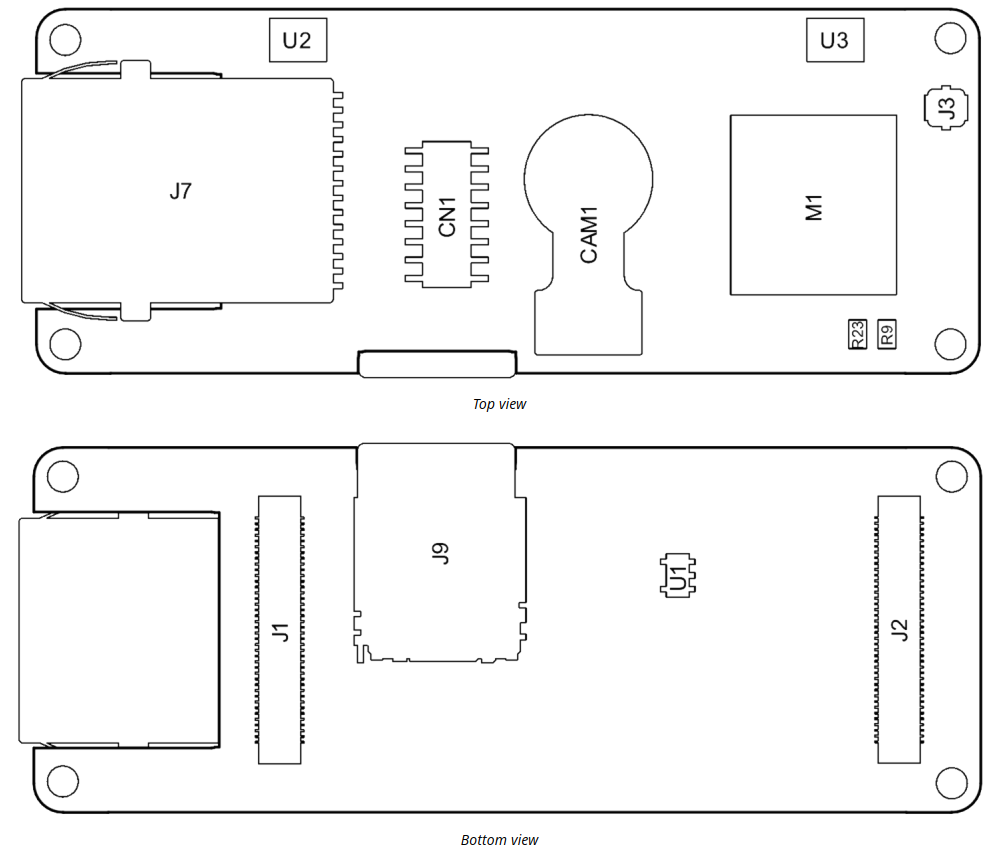
\includegraphics[width=0.7\linewidth]{Images/VisionShield/BoardTopology.png}
		\caption{Board Topology}
		\label{BoardTopology}
	\end{center}
\end{figure}

\begin{figure}
	\begin{center}
		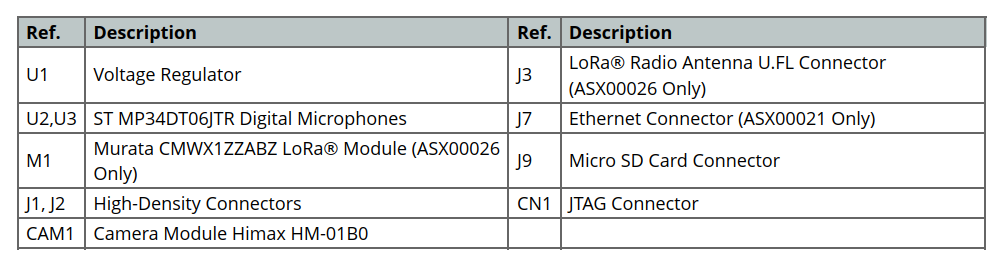
\includegraphics[width=0.7\linewidth]{Images/VisionShield/Discription.png}
		\caption{Board Topology}
		\label{BoardTopology}
	\end{center}
\end{figure}

	
	\section{Power}
	
	The Portenta H7/C33 supplies 3.3 V power to the LoRa\textsuperscript{\textregistered} module (ASX00026 only), Ethernet communication (ASX00021 only), Micro SD slot, and dual microphones via the 3.3 V output of the high-density connectors. An onboard LDO regulator supplies a 2.8 V output (300 mA) for the camera module.
	
	\section{Camera Module}
	
	The Himax HM-01B0 Module is a very low-power camera with 324x324 resolution and a maximum of 60 FPS depending on the operating mode. Video data is transferred over a configurable 8-bit interconnect with support for frame and line synchronization. The module delivered with the Portenta Vision Shield is the monochrome version. Configuration is achieved via an I2C connection with the compatible Portenta boards microcontrollers.
	
	HM-01B0 offers very low-power image acquisition and provides the possibility to perform motion detection without main processor interaction. The “Always-on” operation provides the ability to turn on the main processor when movement is detected with minimal power consumption.
	
	\textbf{Note:} The Portenta C33 is not compatible with the camera of the Portenta Vision Shield.
	
	\section{Digital Microphones}
	
	The dual MP34DT05 digital MEMS microphones are omnidirectional and operate via a capacitive sensing element with a high (64 dB) signal-to-noise ratio. The microphones have been configured to provide separate left and right audio over a single PDM stream.
	
	The sensing element, capable of detecting acoustic waves, is manufactured using a specialized silicon micromachining process dedicated to produce audio sensors.
	
	\section{Micro SD Card Slot}
	
	A Micro SD card slot is available under the Portenta Vision Shield board. Available libraries allow reading and writing to FAT16/32 formatted cards.
	
	\section{Ethernet (ASX00021 Only)}
	
	Ethernet connector allows connecting to 10/100 Base TX networks using the Ethernet PHY available on the Portenta board.
	
\section{First Step with Portenta Vision Shield:}

\subsection{Getting Started With the Portenta Vision Shield Camera}
This tutorial shows you how to capture frames from the Arduino Portenta Vision Shield Camera module and visualize the video output through a Processing sketch. ~\ref{VisionShield} \cite{portentaVisionShieldCamera:2024}
	\begin{figure}
		\begin{center}
			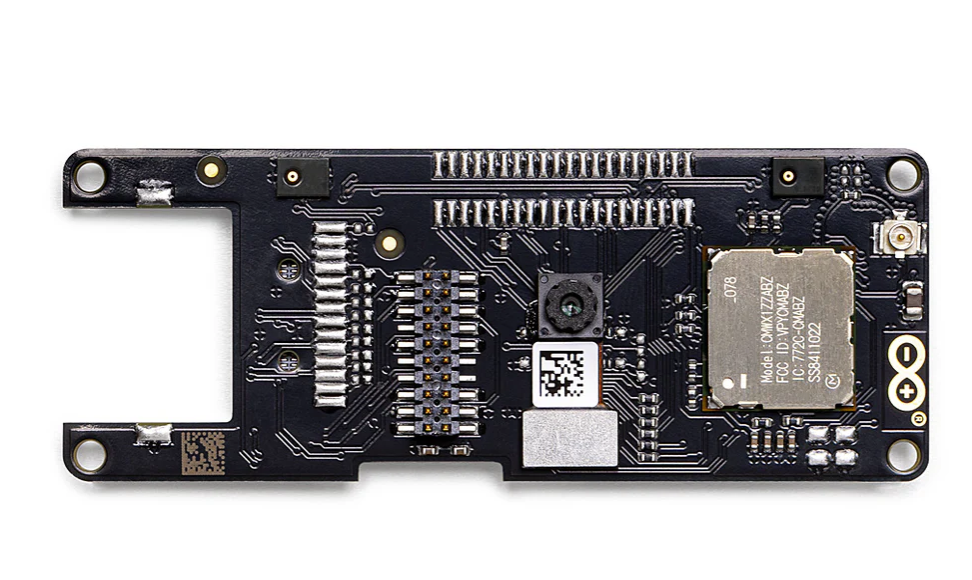
\includegraphics[width=0.7\linewidth]{Images/VisionShield/VisionShield.png}
			\caption{VisionShield}
			\label{VisionShield}
		\end{center}
	\end{figure}

\subsection{Goals:}
\begin{itemize}
	\item Capturing the frames from the camera
	\item Sending the frames as a byte stream through a Serial connection
	\item Visualising the frames in Processing
\end{itemize}

\subsection{Required Hardware and Software:}
\begin{itemize}
	\item Portenta H7
	\item Portenta Vision Shield (LoRa or Ethernet)
	\item USB-C cable
	\item Arduino IDE 2.3.2
	\item Processing software
\end{itemize}
\subsection{Instructions:}
	Accessing the Portenta Vision Shield's camera data is done with the help of both Arduino and the Processing IDE. The Arduino sketch handles the capture of image data by the on-board camera, while the java applet created with Processing helps to visualize this data with the help of a serial connection. The following steps will run you through how to capture, package the data through the serial port and visualize the output in Processing.
\begin{itemize}
	\item \textbf{The Basic Setup:} Connect the Portenta Vision Shield to your Portenta H7 as shown in the figure. The top and bottom high density connecters are connected to the corresponding ones on the underside of the H7 board. Plug in the H7 to your computer using the USB-C® cable. ~\ref{Connection VS}
	\begin{figure}
		\begin{center}
			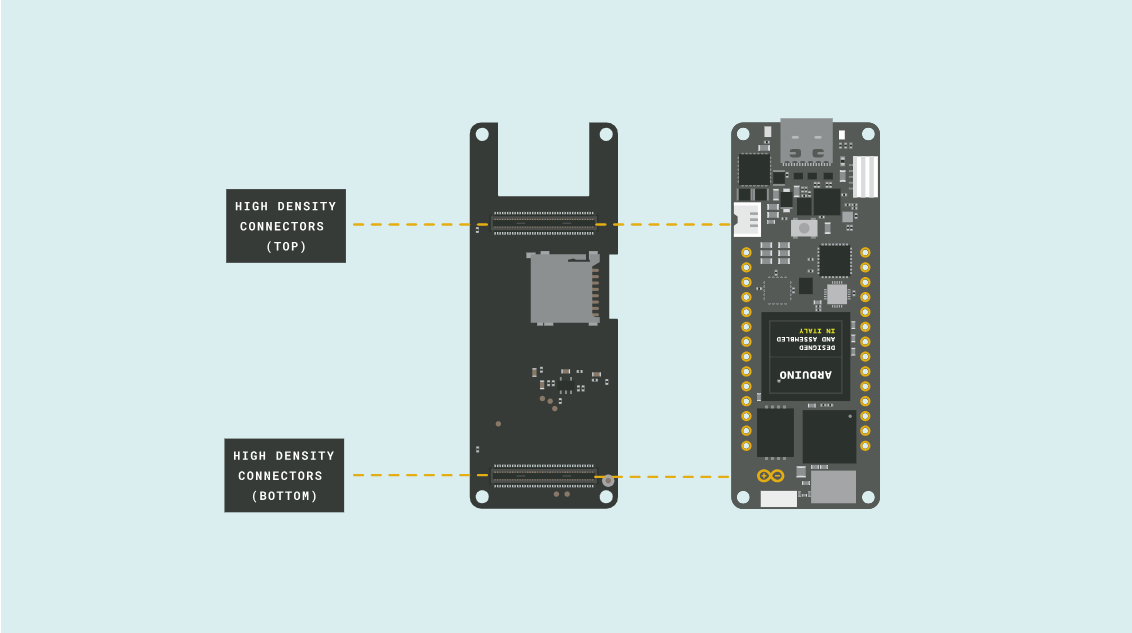
\includegraphics[width=0.7\linewidth]{Images/VisionShield/Connection VS.png}
			\caption{Connection VS}
			\label{Connection VS}
		\end{center}
	\end{figure}
	\item \textbf{Adding the Portenta to the List of Available Boards:} In your Arduino IDE, open the board manager and search for "portenta". Find the Arduino mbed-enabled Boards library and click on "Install" to install the latest version of the mbed core (1.2.3 at the time of writing this tutorial). ~\ref{Portentaport}
	\begin{figure}
		\begin{center}
			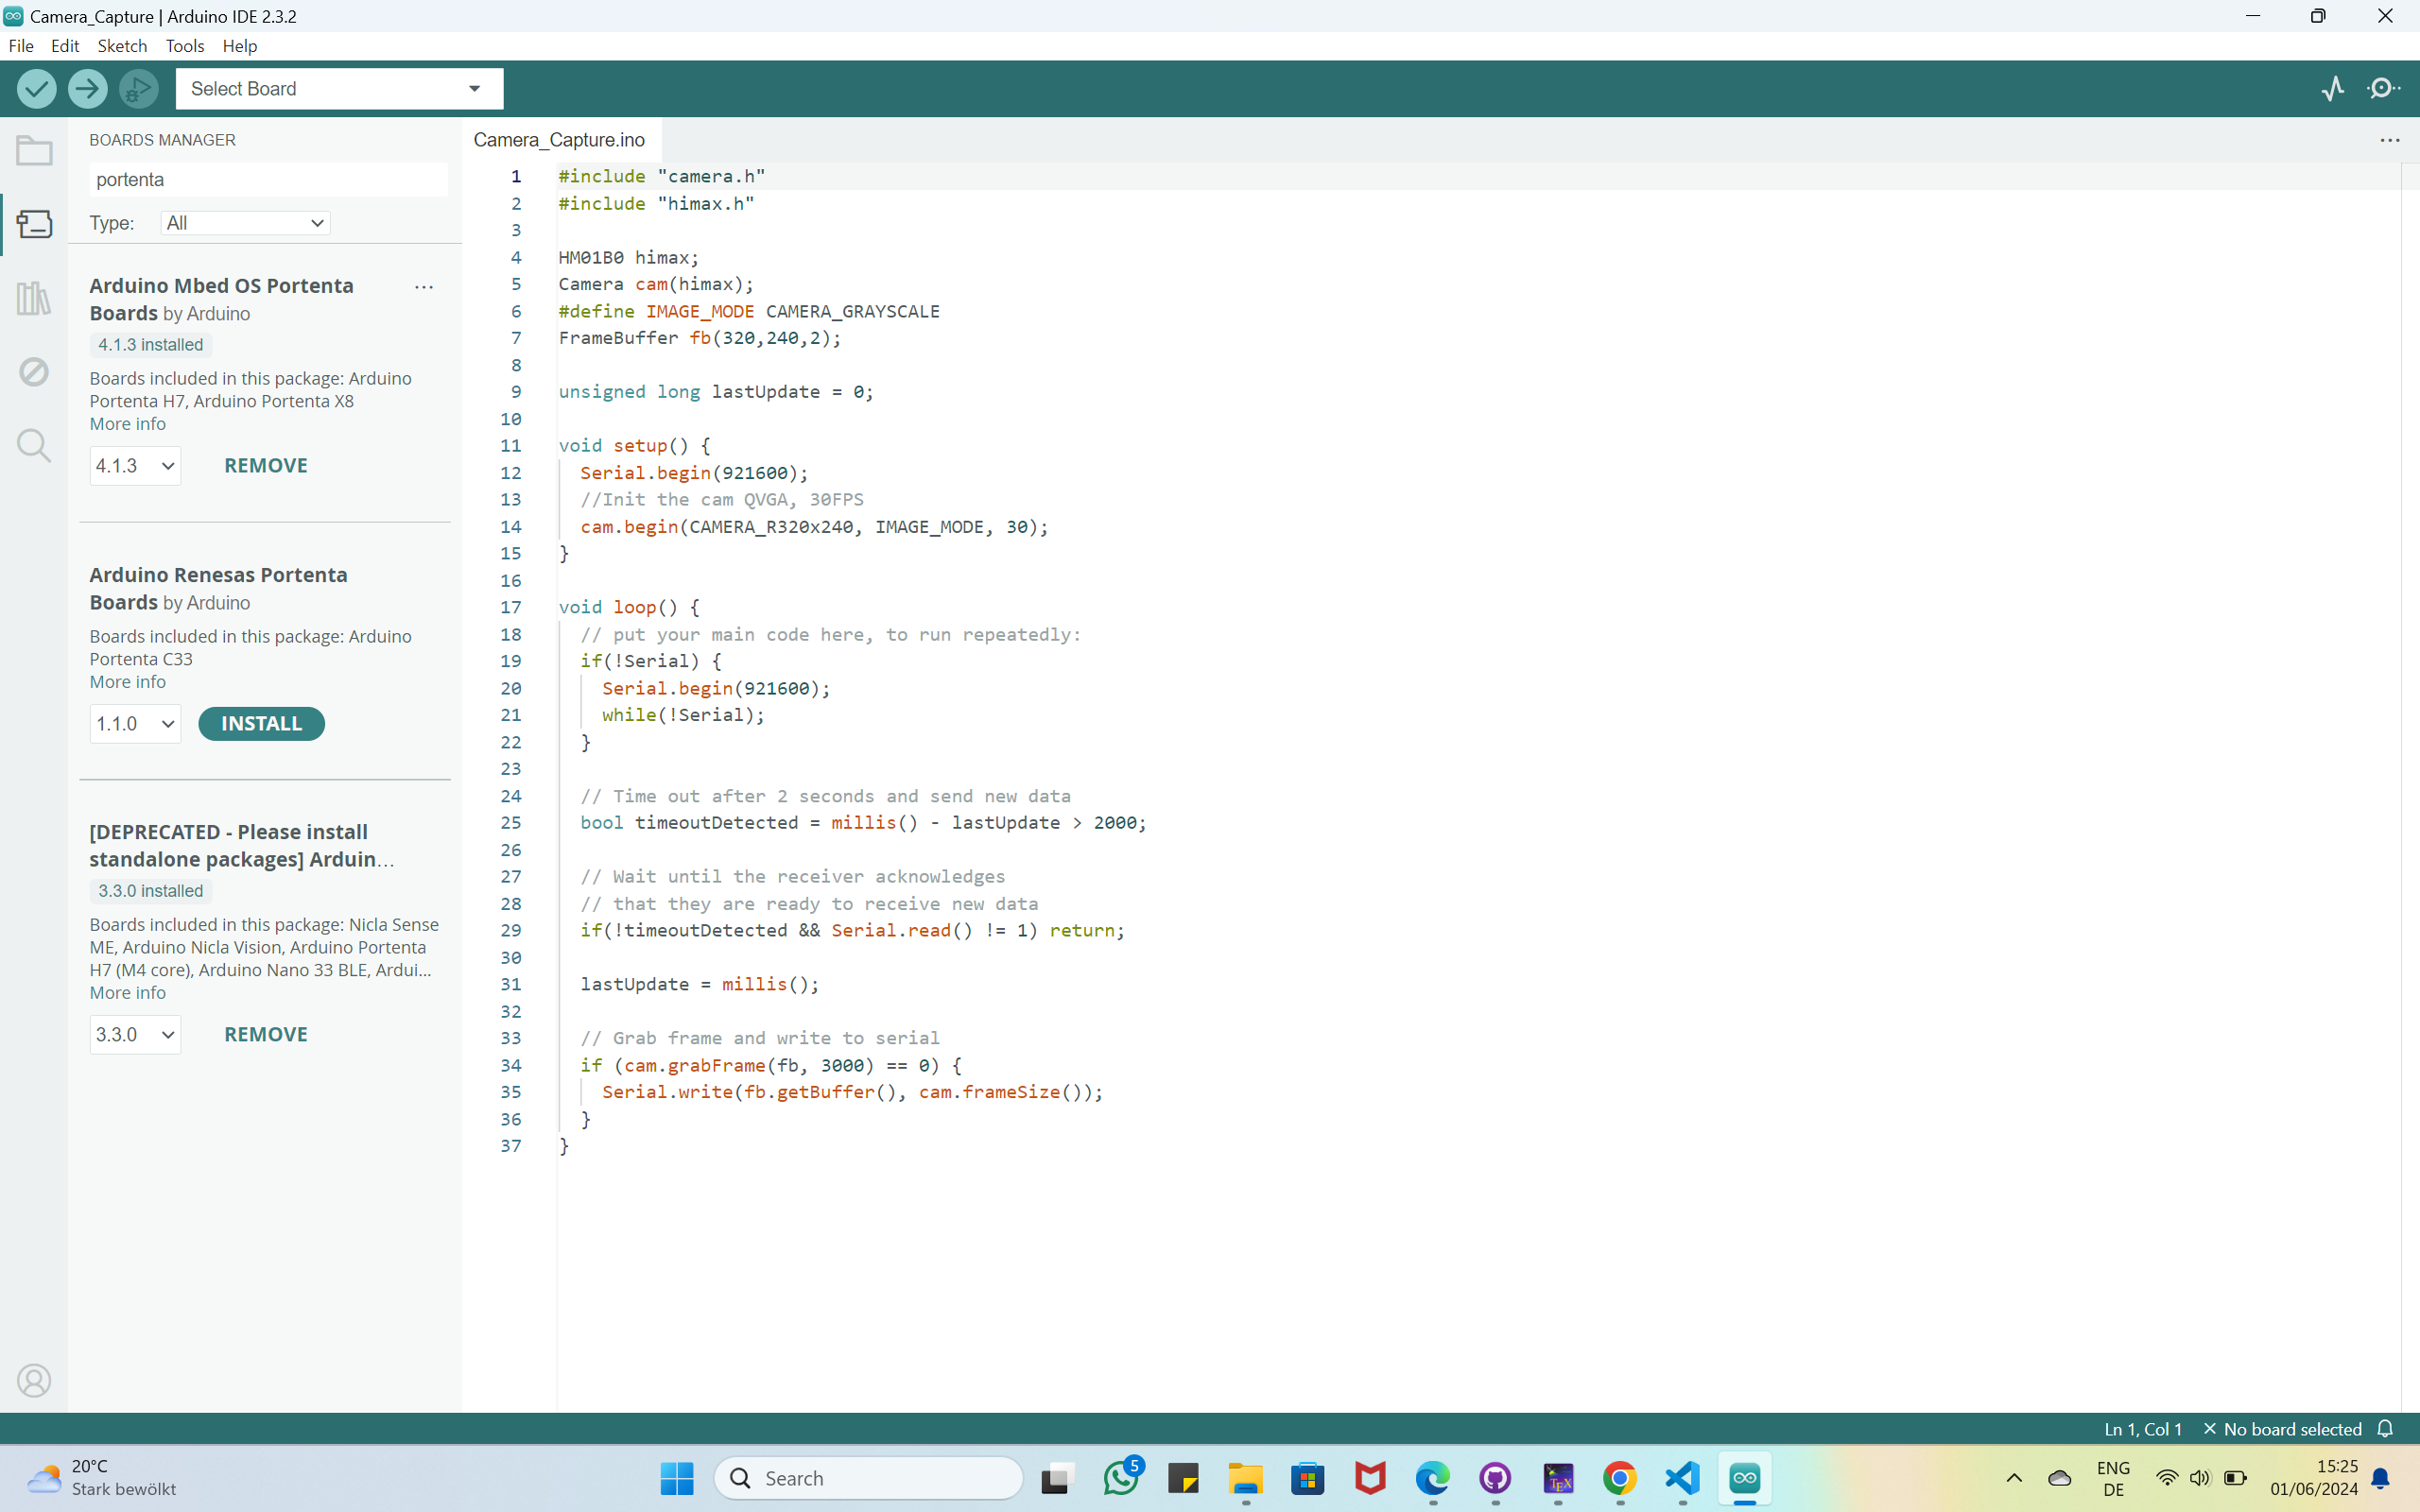
\includegraphics[width=0.7\linewidth]{Images/PortentaH7/Portentaport.png}
			\caption{Portentaport}
			\label{Portentaport}
		\end{center}
	\end{figure}
	
	\item \textbf{Uploading the Classic Blink Sketch:} Let's program the Portenta with the classic blink example to check if the connection to the board works. 
	
	\begin{lstlisting}
		// the setup function runs once when you press reset or power the board
		void setup() {
			// initialize digital pin LED_BUILTIN as an output.
			pinMode(LED_BUILTIN, OUTPUT);
			digitalWrite(LED_BUILTIN, HIGH); // turn the LED off after being turned on by pinMode()
		}
		
		// the loop function runs over and over again forever
		void loop() {
			digitalWrite(LED_BUILTIN, LOW); // turn the LED on (LOW is the voltage level)
			delay(1000); // wait for a second
			digitalWrite(LED_BUILTIN, HIGH); // turn the LED off by making the voltage HIGH
			delay(1000); // wait for a second
		}   
		
	\end{lstlisting}
	
\end{itemize}



\InputLanguage{../Contents/General/}{IMULSM6DS0XTR}

\InputLanguage{../Contents/PortentaH7/}{Proximity}


%\Ausblenden
{
  % Zurzeit nur für Portenta H7
  \InputLanguage{../Contents/General/}{FaceDetectionEdgeImpulse}
}





\chapter{MicroPython \& OpenMV}

\section{MicroPython}



\chapter{First Application: Object Detection}

\chapter{Training a Custom Machine Learning Model for Portenta H7}

\url{https://www.arduino.cc/pro/tutorials/portenta-h7/vs-openmv-ml}

\chapter{Use TensorFlow Lite with Portenta H7}




\part{Anhang}

%%%%%%
%
% $Autor: Wings $
% $Datum: 2020-01-18 11:15:45Z $
% $Pfad: WuSt/Skript/Produktspezifikation/powerpoint/ImageProcessing.tex $
% $Version: 4620 $
%
%%%%%%


\chapter{Materialliste}



%\begin{table}
	\begin{longtable}{cp{6.1cm}p{2.5cm}c}
      \textbf{Anzahl} & \textbf{Bezeichnung} & \textbf{Link} & \textbf{Preis} \\ \hline      
      \multicolumn{4}{c}{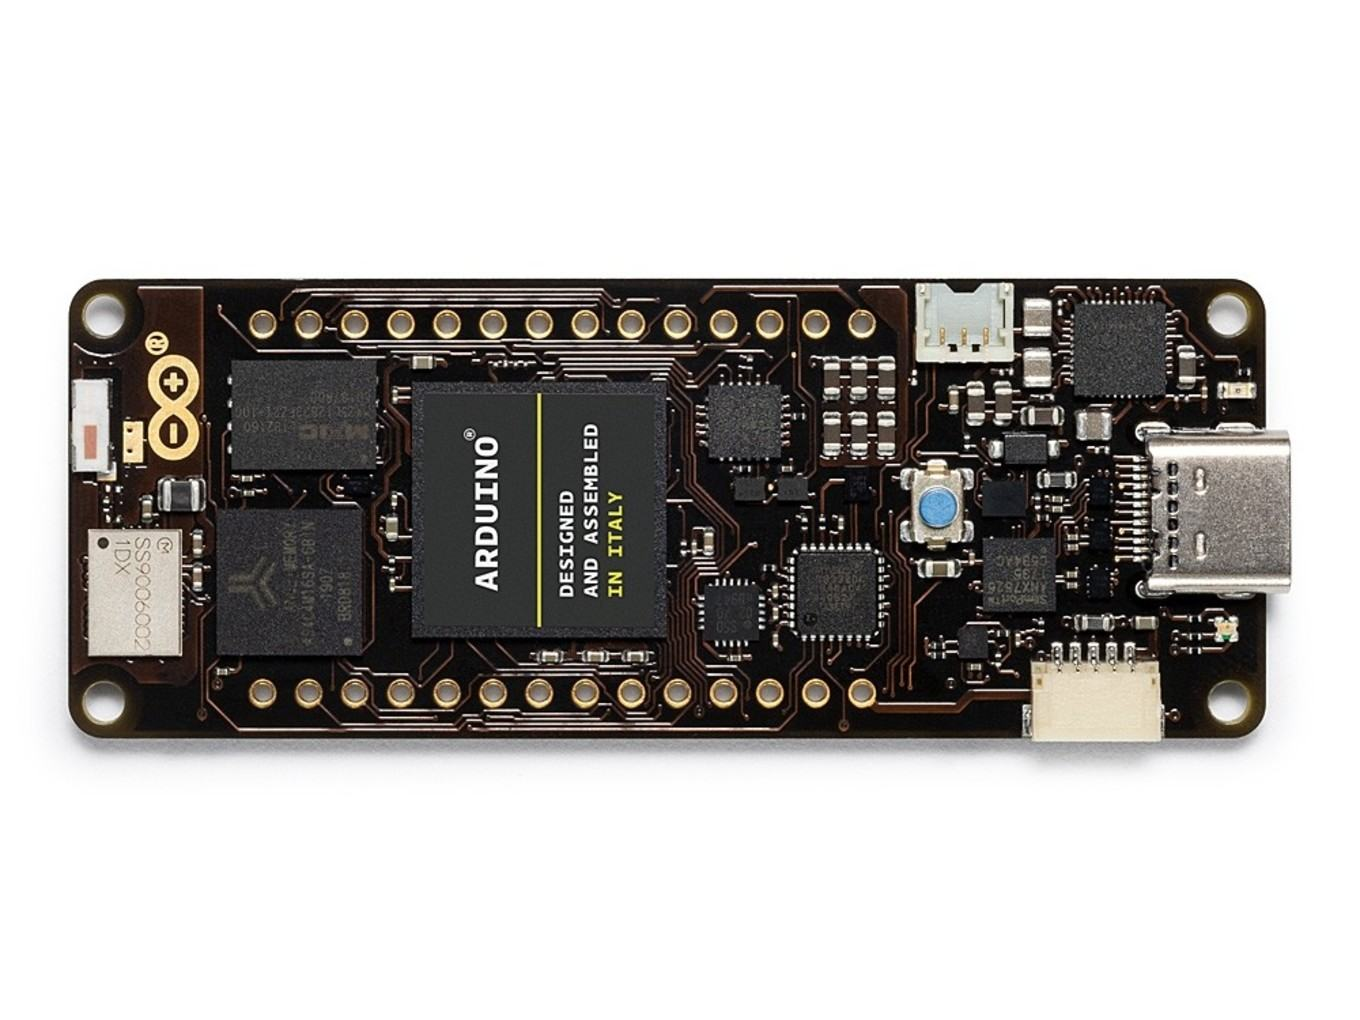
\includegraphics[width=0.2\textwidth]{Arduino/PortentaH7b}} \\
      1      & ARD PORTENTA H7 Arduino Portenta H7, STM32H747, ohne Header
             & \href{https://www.reichelt.de/arduino-portenta-h7-stm32h747-ohne-header-ard-portenta-h7-p292399.html}{www.reichelt.de -  ARD PORTENTA H7} 
             &  97{,}30 \euro{} \\ \hline
      \multicolumn{4}{c}{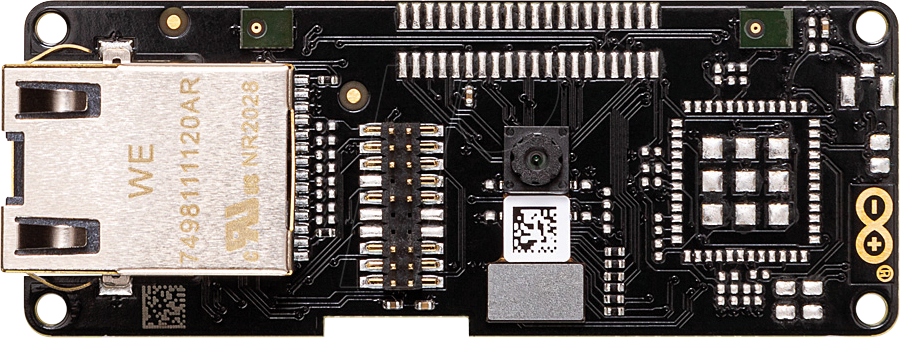
\includegraphics[width=0.2\textwidth]{Arduino/PortentaVisionShield2}} \\
      1       & Arduino Portenta Shield - Vision mit LAN
              & \href{https://www.reichelt.de/arduino-portenta-shield-vision-mit-lan-ard-shd-asx00021-p292402.html}{www.reichelt.de - ARD SHD ASX00021} 
              &  49{,}75 \euro{} \\ \hline
      \multicolumn{4}{c}{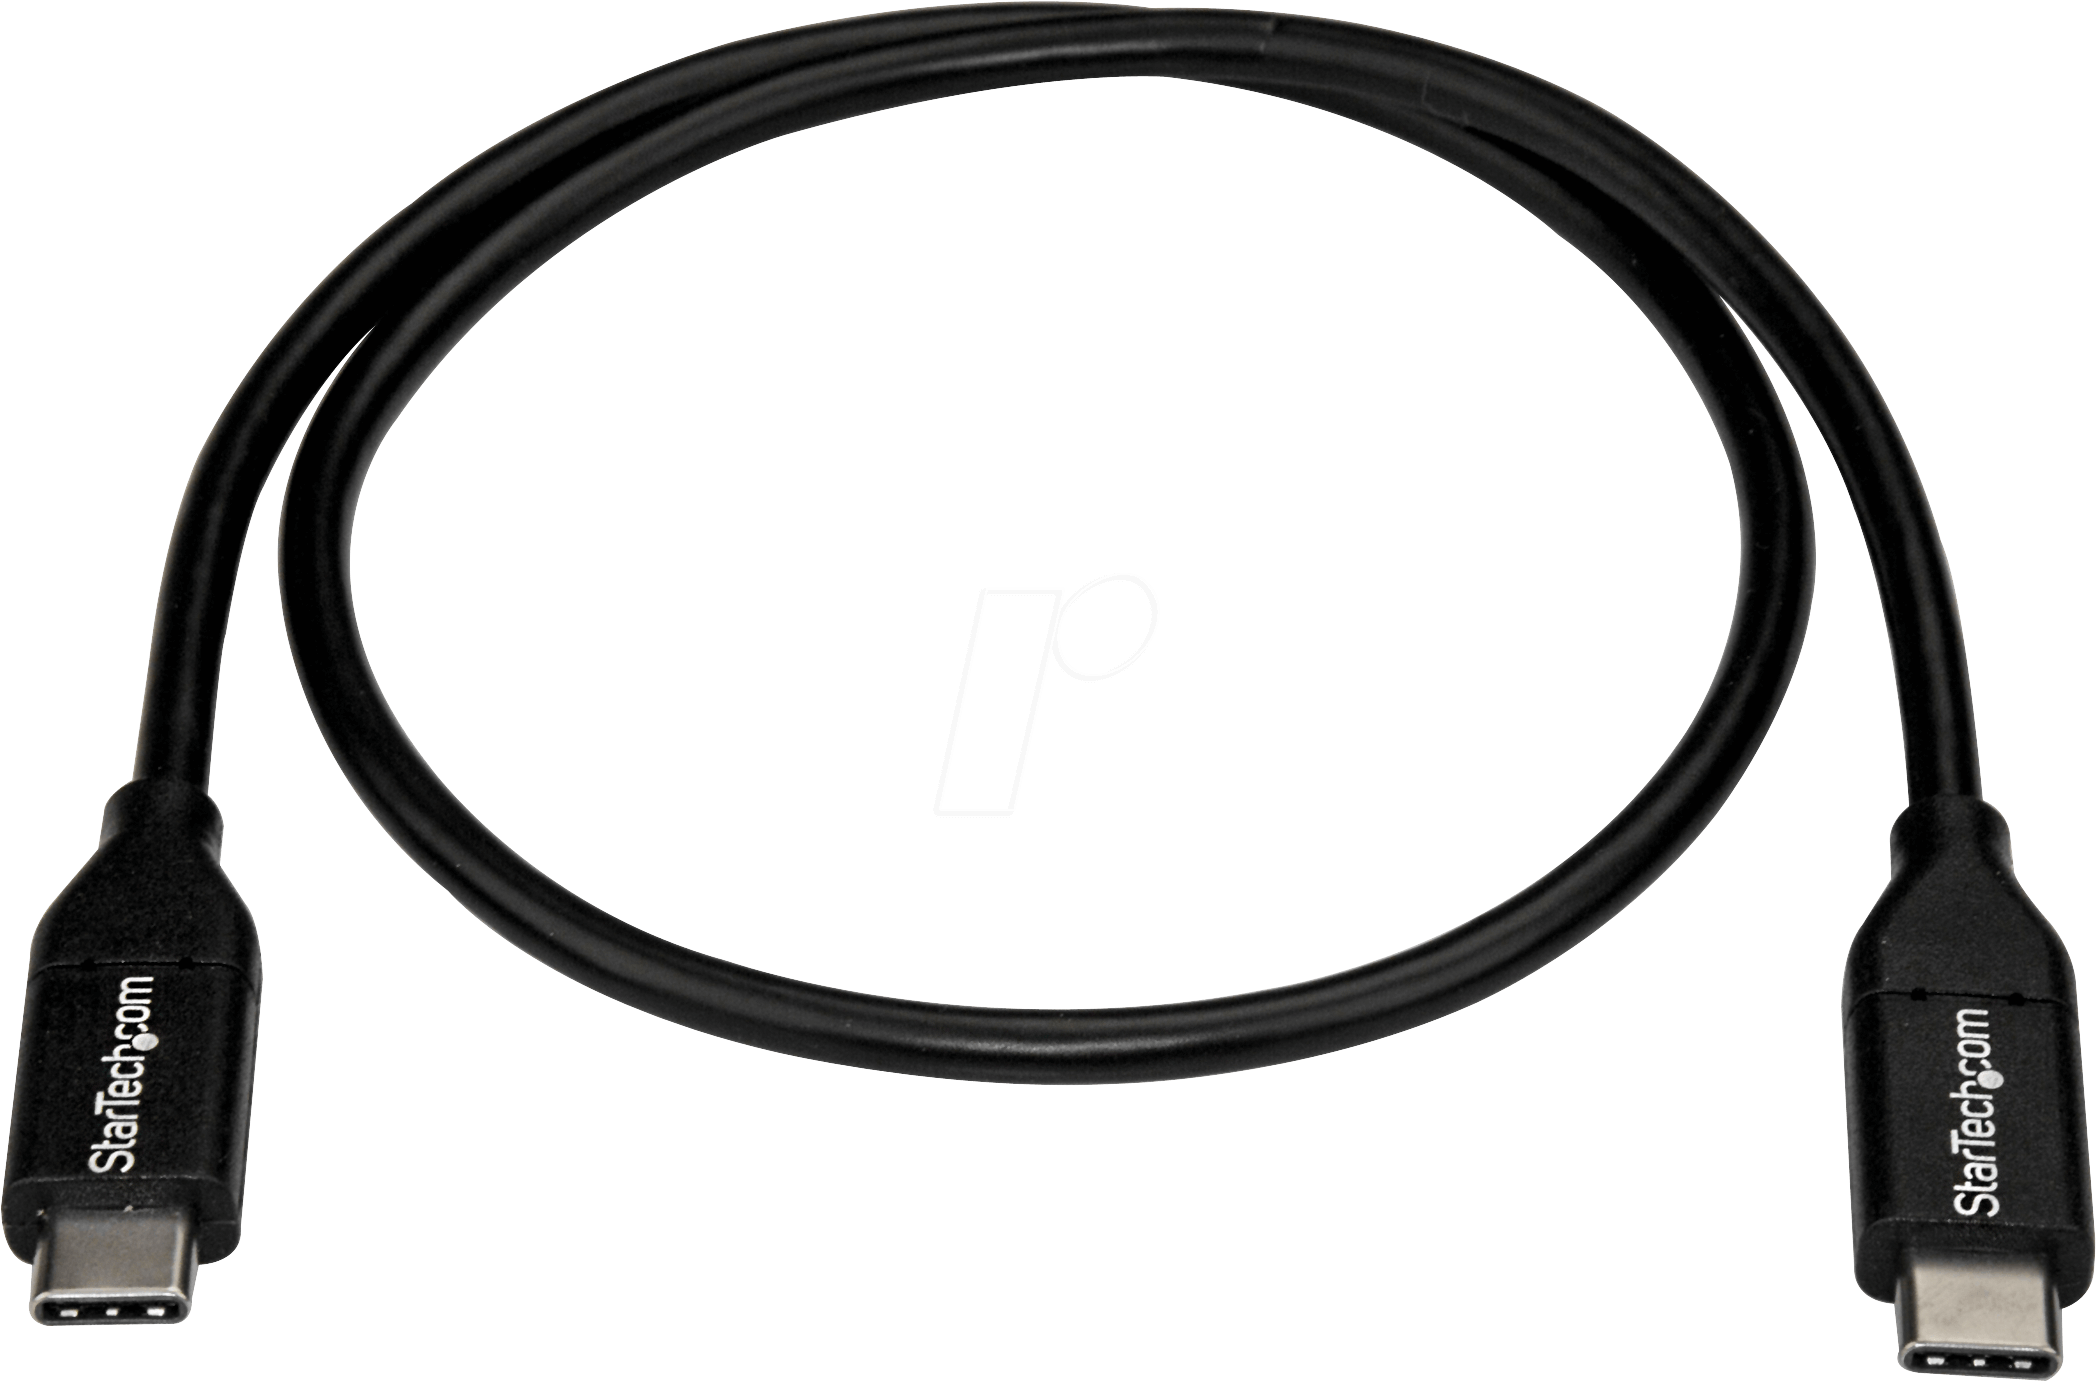
\includegraphics[width=0.2\textwidth]{Arduino/STARTECH_USB2CC50CM_03.png}} \\
      1       & USB 2.0 Kabel USB-C auf USB-C, 0,5 m
              & \href{https://www.reichelt.de/usb-2-0-kabel-usb-c-auf-usb-c-0-5-m-st-usb2cc50cm-p280358.html}{www.reichelt.de - ST USB2CC50CM} 
              &  17{,}20 \euro{} \\ \hline
      \multicolumn{4}{c}{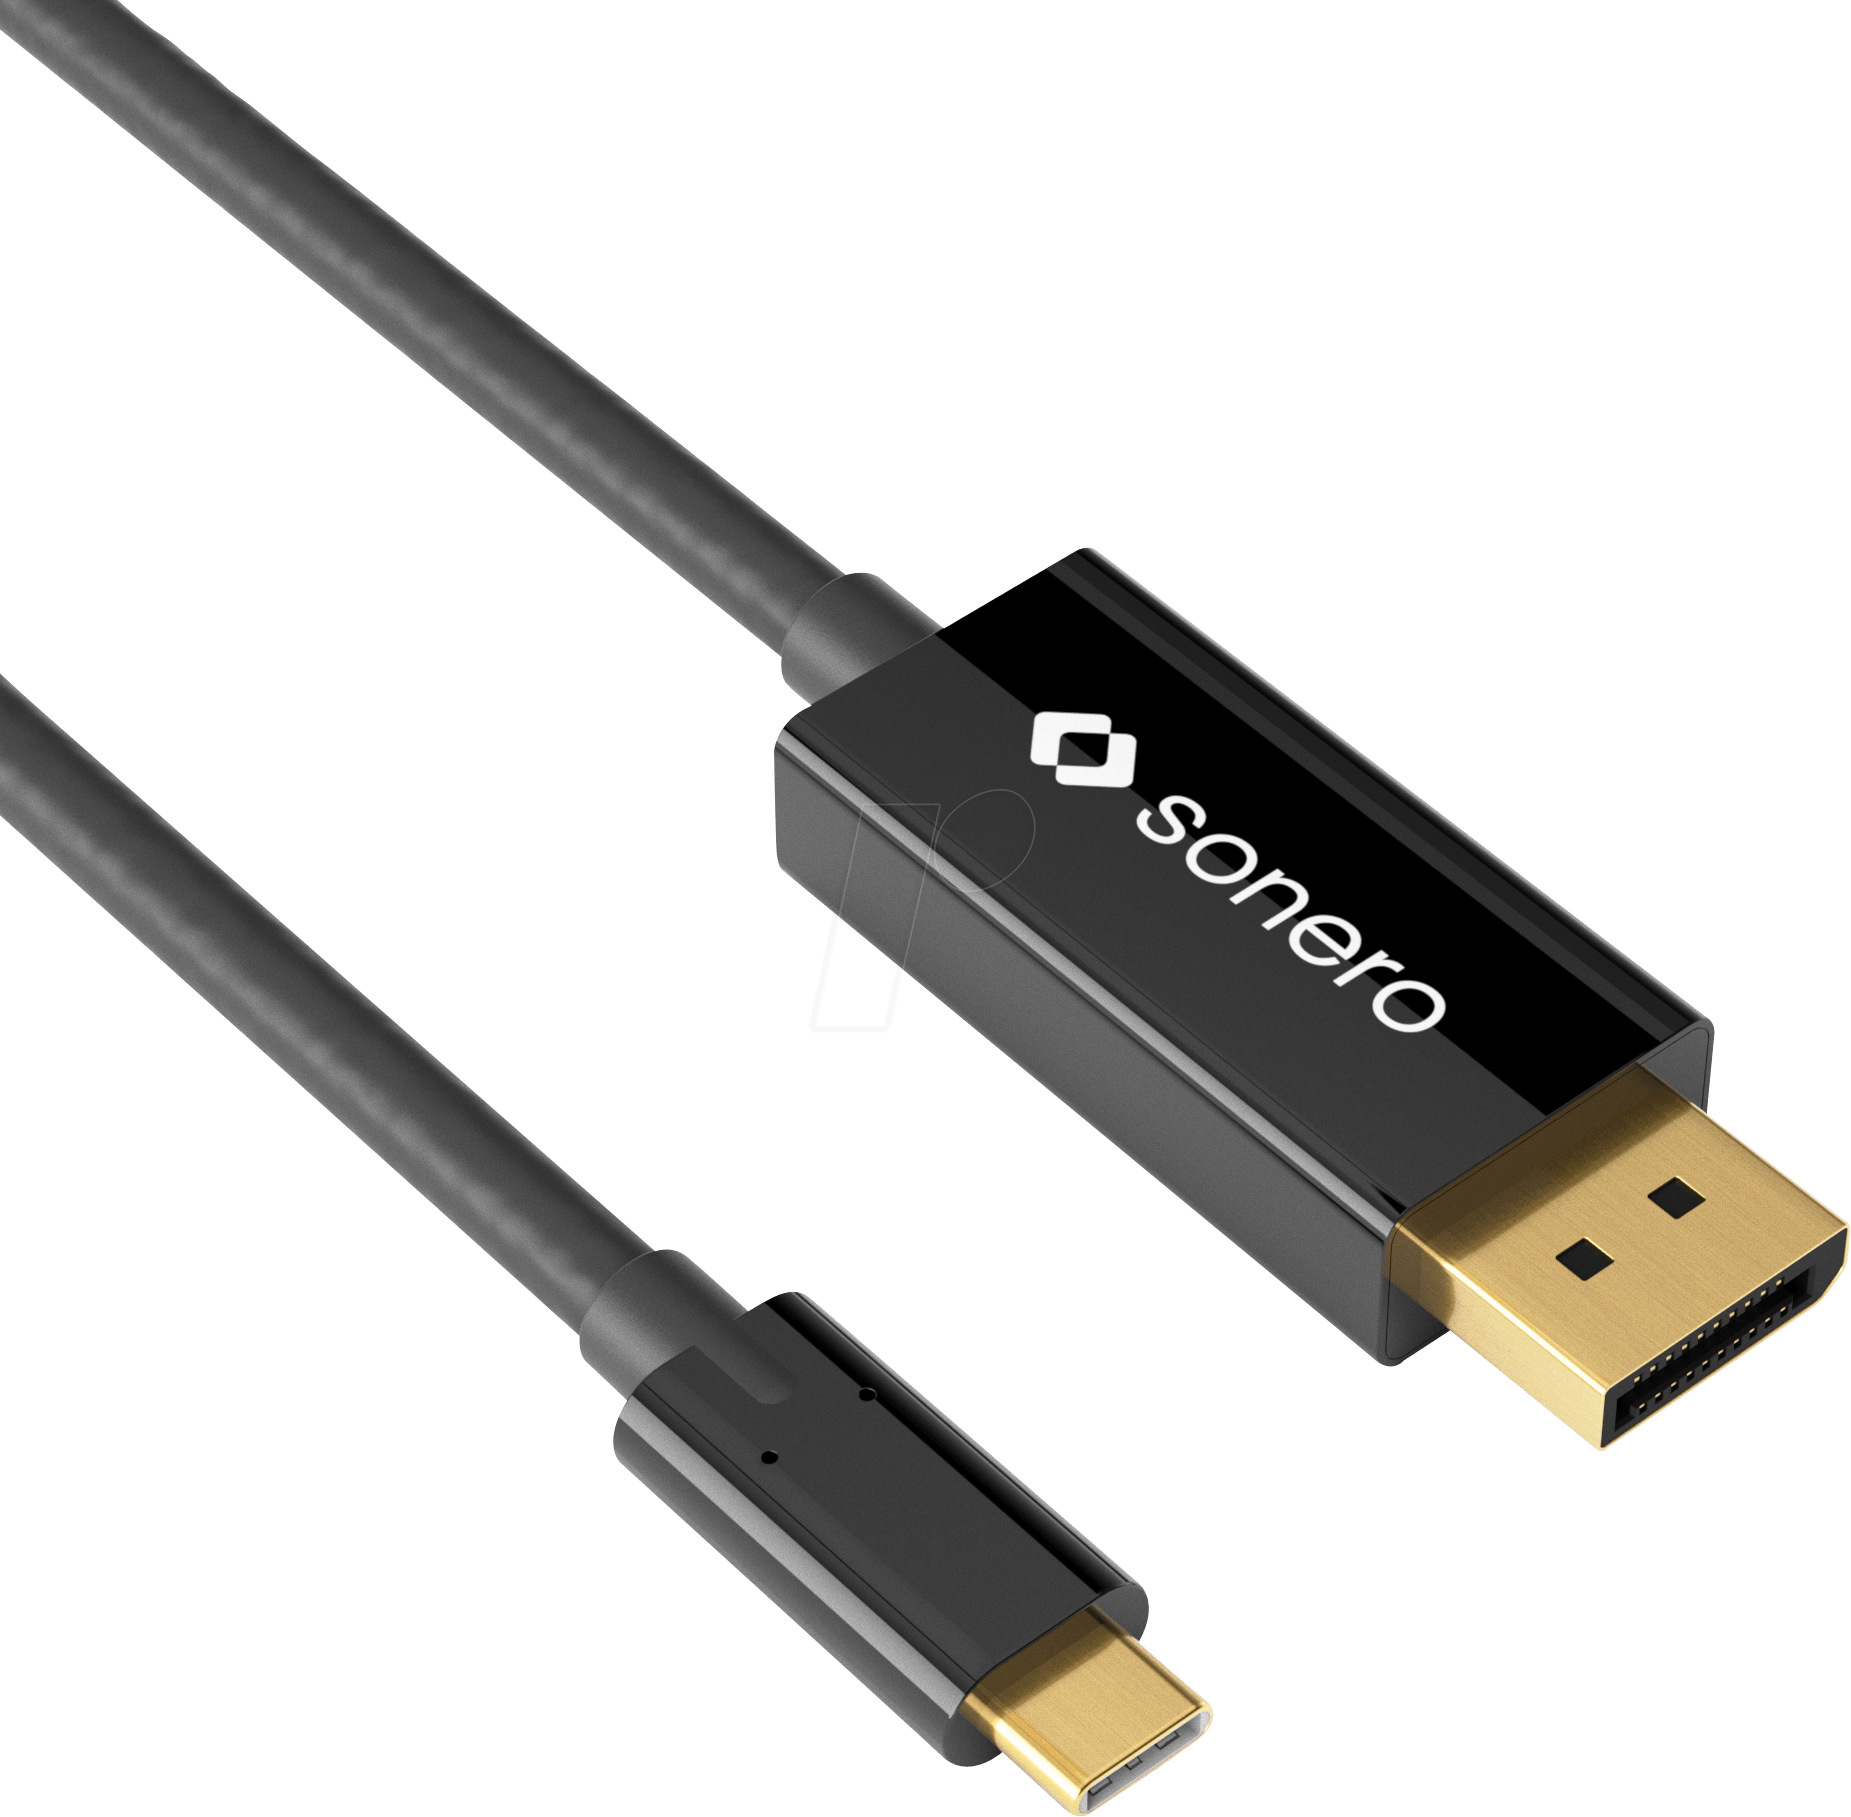
\includegraphics[width=0.2\textwidth]{Arduino/SON_X-UCC020_02}} \\
      1       & USB C Stecker auf DP Kabel, DP Mode, 4K60, 1 m, schwarz
              & \href{https://www.reichelt.de/usb-c-stecker-auf-dp-kabel-dp-mode-4k60-1-m-schwarz-son-x-ucc020-010-p213312.html}{www.reichelt.de - SON X-UCC020-010} 
              &  16{,}90 \euro{} \\ \hline
    1        &  Netzteil 
             & 
             &   \euro{} \\ \hline
    1        &  Monitor
& 
&   \euro{} \\ \hline
    \end{longtable}

Stand: 18.05.2021

%  \caption{Materialliste für die Applikation Bilderkennung}
%\end{table}




%\Ausblenden
{

%%%%%%
%
% $Autor: Wings $
% $Datum: 2020-01-18 11:15:45Z $
% $Pfad: WuSt/Skript/Produktspezifikation/powerpoint/ImageProcessing.tex $
% $Version: 4620 $
%
%%%%%%


\chapter{Datenblätter}

\section{Datenübersicht}

\newcounter{mycounter}

\setcounter{mycounter}{1}

\whiledo {\value{mycounter} < 3}
{
	\includegraphics[width=1\textwidth,page=\themycounter]{../../MLbib/Arduino/PortentaH7/PORTENTA_H7_PRODUCT_DESCRIPTION.pdf}
	\stepcounter{mycounter}
	\newpage
}



\setcounter{mycounter}{1}

\whiledo {\value{mycounter} < 27}
{
  \includegraphics[width=1\textwidth,page=\themycounter]{../../MLbib/Arduino/PortentaH7/Pinout-PortentaH7_latest.pdf}
  \stepcounter{mycounter}
  \newpage
}

\setcounter{mycounter}{1}

\whiledo {\value{mycounter} < 12}
{
	\includegraphics[width=1\textwidth,page=\themycounter]{../../MLbib/Arduino/PortentaH7/Arduino-PortentaH7-schematic-V10.pdf}
	\stepcounter{mycounter}
	\newpage
}

\setcounter{mycounter}{1}

\whiledo {\value{mycounter} < 12}
{
	\includegraphics[width=1\textwidth,page=\themycounter]{../../MLbib/Arduino/PortentaH7/Portenta_H7_Web.pdf}
	\stepcounter{mycounter}
	\newpage
}




%%%%%%
%
% $Autor: Wings $
% $Datum: 2020-01-18 11:15:45Z $
% $Pfad: WuSt/Skript/Produktspezifikation/powerpoint/ImageProcessing.tex $
% $Version: 4620 $
%
%%%%%%


\chapter{Datenblätter Arduino Vision Shield}


\newcounter{VScounter}
\setcounter{VScounter}{1}

\whiledo {\value{VScounter} < 4}
{
	\includegraphics[width=1\textwidth,page=\theVScounter]{../../MLbib/Arduino/PortentaH7/ARD_SHD_ASX0002X_DATASHEET.pdf}
	\stepcounter{VScounter}
	\newpage
}

\setcounter{VScounter}{1}

\whiledo {\value{VScounter} < 18}
{
	\includegraphics[width=1\textwidth,page=\theVScounter]{../../MLbib/Arduino/PortentaH7/ASX00021-ASX00026-DB_EN.pdf}
	\stepcounter{VScounter}
	\newpage
}


}

%\addcontentsline{toc}{chapter}{Literaturverzeichnis}

\printbibliography[
heading=bibintoc,
title={Literaturverzeichnis}
]


\newpage

\addcontentsline{toc}{chapter}{Stichwortverzeichnis}
\printindex

%\part{Anhang}


%%\chapter{Todo List}
\hypertarget{todo}{}\label{todo}\index{Todo List@{Todo List}}

\begin{DoxyRefList}
\item[Member \doxylink{group___n_n_conv_ga6c569efc46ae1c38df1335888fc7873d}{arm\+\_\+convolve\+\_\+1\+\_\+x\+\_\+n\+\_\+s8} (const \doxylink{structcmsis__nn__context}{cmsis\+\_\+nn\+\_\+context} \texorpdfstring{$\ast$}{*}ctx, const \doxylink{structcmsis__nn__conv__params}{cmsis\+\_\+nn\+\_\+conv\+\_\+params} \texorpdfstring{$\ast$}{*}conv\+\_\+params, const \doxylink{structcmsis__nn__per__channel__quant__params}{cmsis\+\_\+nn\+\_\+per\+\_\+channel\+\_\+quant\+\_\+params} \texorpdfstring{$\ast$}{*}quant\+\_\+params, const \doxylink{structcmsis__nn__dims}{cmsis\+\_\+nn\+\_\+dims} \texorpdfstring{$\ast$}{*}input\+\_\+dims, const q7\+\_\+t \texorpdfstring{$\ast$}{*}input\+\_\+data, const \doxylink{structcmsis__nn__dims}{cmsis\+\_\+nn\+\_\+dims} \texorpdfstring{$\ast$}{*}filter\+\_\+dims, const q7\+\_\+t \texorpdfstring{$\ast$}{*}filter\+\_\+data, const \doxylink{structcmsis__nn__dims}{cmsis\+\_\+nn\+\_\+dims} \texorpdfstring{$\ast$}{*}bias\+\_\+dims, const int32\+\_\+t \texorpdfstring{$\ast$}{*}bias\+\_\+data, const \doxylink{structcmsis__nn__dims}{cmsis\+\_\+nn\+\_\+dims} \texorpdfstring{$\ast$}{*}output\+\_\+dims, q7\+\_\+t \texorpdfstring{$\ast$}{*}output\+\_\+data)]\hfill \\
\label{todo__todo000001}%
\Hypertarget{todo__todo000001}%
Remove constraint on output\+\_\+dims-\/\texorpdfstring{$>$}{>}w to make the function generic.

\label{todo__todo000002}%
\Hypertarget{todo__todo000002}%
Remove constraint on output\+\_\+dims-\/\texorpdfstring{$>$}{>}w to make the function generic. 
\item[Class \doxylink{classei_1_1signal}{ei\+::signal} ]\hfill \\
\label{todo__todo000003}%
\Hypertarget{todo__todo000003}%
\+: call CMSIS DSP functions if available 
\end{DoxyRefList}
%


\end{document}
